\documentclass[12pt,openright]{book}

\newlength{\margIn}
\newlength{\margOut}
\newlength{\margTop}
\newlength{\margBot}

% \usepackage{emptypage}
% \setlength{\margIn}{3cm}
% \setlength{\margOut}{2cm}
% \setlength{\margTop}{3cm}
% \setlength{\margBot}{2.5cm}
% \PassOptionsToPackage{a4paper}{geometry}

\renewcommand{\cleardoublepage}{\clearpage}
\setlength{\margIn}{.5cm}
\setlength{\margOut}{.5cm}
\setlength{\margTop}{.5cm}
\setlength{\margBot}{.5cm}
\PassOptionsToPackage{paperwidth=17cm, paperheight=25.2cm}{geometry}

\PassOptionsToPackage{english,main=indonesian}{babel}
\PassOptionsToPackage{autostyle}{csquotes}
\PassOptionsToPackage{inner=\margIn, outer=\margOut, top=\margTop, bottom=\margBot}{geometry}
\PassOptionsToPackage{hidelinks}{hyperref}
\PassOptionsToPackage{authoryear}{natbib}
\PassOptionsToPackage{table,xcdraw}{xcolor}

\usepackage{
	babel,
	csquotes,
	textcase,
	amsthm,
	lmodern,
	newtxtext,
	newtxmath,
	newtxtt,
	fancyvrb,
	geometry,
	pagecolor,
	% parskip,
	indentfirst,
	titlesec,
	titletoc,
	tabularx,
	array,
	multirow,
	float,
	graphicx,
	wrapfig,
	wallpaper,
	subcaption,
	xcolor,
	ulem,
	tikz,
	% pdflscape,
	lscape,
	hyperref,
	xurl,
	cleveref,
	natbib,
	fancyhdr,
	algorithm
}

\def\True{\mathtt{True}}
\def\False{\mathtt{False}}

\newcommand{\foreign}[1]{\foreignlanguage{english}{\textit{#1}}}

\theoremstyle{definition}
\newtheorem{examplex}{Contoh}

\newenvironment{example}
	{\begin{examplex}\pushQED{\qed}}
	{\popQED\end{examplex}}

\addto\extrasindonesian{
	\renewcommand{\chapterautorefname}{Bab}
	\renewcommand{\sectionautorefname}{Subbab}
	\renewcommand{\subsectionautorefname}{Subsubbab}
	\renewcommand{\figureautorefname}{Gambar}
	\renewcommand{\tableautorefname}{Tabel}
	\renewcommand{\equationautorefname}{Persamaan}
	\floatname{algorithm}{Algoritma}
	\renewcommand{\refname}{Daftar Pustaka}
	\renewcommand{\bibname}{Daftar Pustaka}
	\providecommand{\algorithmautorefname}{Algoritma}
	\providecommand{\examplexautorefname}{Contoh}
	\crefname{appsec}{Lampiran}{Appendices}
	\Crefname{appsec}{Lampiran}{Appendices}
}

\newcommand{\bulan}[1]{
	\ifcase#1\relax
		\or Januari\or Februari\or Maret\or April\or Mei\or Juni\or Juli\or Agustus\or September\or Oktober\or Nopember\or Desember%
	\fi
}

\captionsetup{hypcap=false}

\titleformat{\chapter}[display]
	{\centering\large\bfseries}
	{\MakeUppercase{\chaptername~\Roman{chapter}}}
	{0pt}
	{\MakeUppercase}

\titlespacing*{\chapter}
	{0pt}
	{0.5\baselineskip}
	{2\baselineskip}

\titleformat{\section}
	{\normalfont\bfseries}
	{\thesection}
	{1em}
	{}

\titlespacing*{\section}
	{0pt}
	{0.5\baselineskip}
	{0.2\baselineskip}

\titleformat{\subsection}
	{\normalfont\bfseries}
	{\thesubsection}
	{1em}
	{}

\titlespacing*{\subsection}
	{0pt}
	{0.5\baselineskip}
	{0.2\baselineskip}

\titlecontents{chapter}[0pt]
	{\vspace{0.5em}}
	{BAB \MakeUppercase{\romannumeral\thecontentslabel}\quad\MakeUppercase}
	{\MakeUppercase}
	{\hfill\contentspage}

\titlecontents{figure}[1.5em]
	{}
	{Gambar \makebox[2em][l]{\thecontentslabel}\enspace}
	{}
	{\ \titlerule*[.75pc]{.}\contentspage}

\titlecontents{table}[1.5em]
	{}
	{Tabel \makebox[2em][l]{\thecontentslabel}\enspace}
	{}
	{\ \titlerule*[.75pc]{.}\contentspage}

\raggedbottom

\renewcommand{\headrulewidth}{0pt}

\newcommand\abspagenumber{\inteval{\ReadonlyShipoutCounter+1}}

\newcommand{\margRepair}{
	\ifodd\abspagenumber
		\newgeometry{inner=\margIn, outer=\margOut, top=\margTop, bottom=\margBot}
	\else
		\newgeometry{inner=\margOut, outer=\margIn, top=\margTop, bottom=\margBot}
	\fi
}

\newcommand{\footRepair}{
	\ifodd\abspagenumber
		\fancyhf{}
		\fancypagestyle{plain}{\fancyfoot[RO,LE]{\thepage}}
		\pagestyle{plain}
	\else
		\fancyhf{}
		\fancypagestyle{plain}{\fancyfoot[RE,LO]{\thepage}}
		\pagestyle{plain}
	\fi
}

\let\ORIGINALfrontmatter\frontmatter
\let\ORIGINALmainmatter\mainmatter
\renewcommand{\frontmatter}{\ORIGINALfrontmatter \margRepair \footRepair}
\renewcommand{\mainmatter}{\ORIGINALmainmatter \margRepair \footRepair}



\newcommand{\titleBahasa}{Menentukan Dimensi Metrik Menggunakan \foreign{Satisfiability Modulo Theories}}

\newcommand{\titleEnglish}{Determining Metric Dimension with Satisfiability Modulo Theories}

\newcommand{\theAuthor}{Fikri Yudhistira Ajiwijaya}
\newcommand{\theAuthorId}{5002211165}

\newcommand{\supervisor}{Muhammad Syifa'ul Mufid S.Si, M.Si, Ph.D}
\newcommand{\supervisorId}{198909112014041001}

\newcommand{\examinerOne}{Dr. Dieky Adzkiya, S.Si, M.Si}
\newcommand{\examinerOneId}{198305172008121003}

\newcommand{\examinerTwo}{Soleha, S.Si, M.Si}
\newcommand{\examinerTwoId}{198301072006042001}

\newcommand{\examinerThree}{Muhammad Luthfi Shahab, S.Si, M.Si, Ph.D}
\newcommand{\examinerThreeId}{199503312018031001}

\newcommand{\programChair}{Dr. Tahiyatul Asfihani, S.Si, M.Si}
\newcommand{\programChairId}{198707282014042001}
\newcommand{\programChairTitle}{Kepala Proram Studi Sarjana}

\newcommand{\documentName}{Tugas Akhir}
\newcommand{\degreeName}{Sarjana Matematika}
\newcommand{\programName}{Program Studi S-1 Matematika}
\newcommand{\departmentName}{Departemen Matematika}
\newcommand{\facultyName}{Fakultas Sains dan Analitika Data}
\newcommand{\facultyNameAbbreviated}{FSAD}
\newcommand{\campusName}{Institut Teknologi Sepuluh Nopember}
\newcommand{\campusNameAbbreviated}{ITS}

\newcommand{\theCity}{Surabaya}
\newcommand{\theDay}{\the\day}
\newcommand{\theMonth}{\bulan{\the\month}}
\newcommand{\theYear}{\the\year}

\title{\titleBahasa}
\author{https://github.com/wijayarakhmat98/metric-dimension}


\begin{document}
	\setlength{\abovedisplayskip}{0.5\baselineskip}
	\setlength{\belowdisplayskip}{0.5\baselineskip}

	\begin{titlepage}
	\newgeometry{inner=\marginOuter, outer=\marginOuter, top=\marginOuter, bottom=\marginOuter}
	\thispagestyle{empty}
	\setlength{\parindent}{0pt}
	\setlength{\parskip}{0.5\baselineskip}
	\color{white}

	\begin{tikzpicture}[remember picture, overlay]
		\fill[itsBlue]
			([yshift=-\dimexpr (4cm + \marginOuter) \relax]current page.north west)
			rectangle
			(current page.south east);
	\end{tikzpicture}%
	
\includegraphics[height=2.5cm]{img/logo-blue.png}

	\vspace{2em}

	{
		\color{itsBlue}
		\makebox[\linewidth]{\rule{30cm}{1cm}}%
	}

	\vspace{2em}

	\hspace{2.5em}\textsf{\textbf{\MakeUppercase{\documentNameBahasa} - \documentCode}}

	\vfill

	\hfill
	\begin{minipage}[t][2cm]{\dimexpr \linewidth - 2.5em \relax}
		\raggedright
		\Large
		\textsf{\textbf{\MakeUppercase{\titleBahasa}}}

		%
	\end{minipage}

	\vfill

	\hspace{2.5em}\textsf{\textbf{\MakeUppercase{\theAuthor}}}

	\hspace{2.5em}\textsf{NRP \theAuthorId}

	\vfill

	\hspace{2.5em}\textsf{Dosen Pembimbing}

	\hspace{2.5em}\textsf{\textbf{\supervisor}}

	\hspace{2.5em}\textsf{NIP \supervisorId}

	\vfill

	\hspace{2.5em}\textsf{\textbf{\degreeLevelBahasa}}

	\hspace{2.5em}\textsf{\departmentNameBahasa}

	\hspace{2.5em}\textsf{\facultyNameBahasa}

	\hspace{2.5em}\textsf{\campusName}

	\hspace{2.5em}\textsf{\theCity}

	\hspace{2.5em}\textsf{\theYear}

	\restoregeometry
\end{titlepage}

	\cleardoublepage

	\begin{titlepage}
	\newgeometry{inner=\marginOuter, outer=\marginOuter, top=\marginOuter, bottom=\marginOuter}
	\thispagestyle{empty}
	\setlength{\parindent}{0pt}
	\setlength{\parskip}{0.5\baselineskip}

	
\includegraphics[height=2.5cm]{img/logo-classic.png}

	\vspace{2em}

	{
		\color{itsBlue}
		\makebox[\linewidth]{\rule{30cm}{1cm}}%
	}

	\vspace{2em}

	\hspace{2.5em}\textsf{\textbf{\MakeUppercase{\documentNameBahasa} - \documentCode}}

	\vfill

	\hfill
	\begin{minipage}[t][2cm]{\dimexpr \linewidth - 2.5em \relax}
		\raggedright
		\Large
		\textsf{\textbf{\MakeUppercase{\titleBahasa}}}

		%
	\end{minipage}

	\vfill

	\hspace{2.5em}\textsf{\textbf{\MakeUppercase{\theAuthor}}}

	\hspace{2.5em}\textsf{NRP \theAuthorId}

	\vfill

	\hspace{2.5em}\textsf{Dosen Pembimbing}

	\hspace{2.5em}\textsf{\textbf{\supervisor}}

	\hspace{2.5em}\textsf{NIP \supervisorId}

	\vfill

	\hspace{2.5em}\textsf{\textbf{\degreeLevelBahasa}}

	\hspace{2.5em}\textsf{\departmentNameBahasa}

	\hspace{2.5em}\textsf{\facultyNameBahasa}

	\hspace{2.5em}\textsf{\campusName}

	\hspace{2.5em}\textsf{\theCity}

	\hspace{2.5em}\textsf{\theYear}

	\restoregeometry
\end{titlepage}

	\cleardoublepage

	\begin{titlepage}
	\newgeometry{inner=\margOut, outer=\margOut, top=\margOut, bottom=\margOut}
	\thispagestyle{empty}
	\setlength{\parindent}{0pt}
	\setlength{\parskip}{0.5\baselineskip}

	
\includegraphics[height=2.5cm]{img/logo-classic.png}

	\vspace{2em}

	{
		\color{itsBlue}
		\makebox[\linewidth]{\rule{30cm}{1cm}}%
	}

	\vspace{2em}

	\hspace{2.5em}\textsf{\textbf{\MakeUppercase{\documentNameEnglish} - \documentCode}}

	\vfill

	\hfill
	\begin{minipage}[t][2cm]{\dimexpr \linewidth - 2.5em \relax}
		\raggedright
		\Large
		\textsf{\textbf{\MakeUppercase{\titleEnglish}}}

		%
	\end{minipage}

	\vfill

	\hspace{2.5em}\textsf{\textbf{\MakeUppercase{\theAuthor}}}

	\hspace{2.5em}\textsf{NRP \theAuthorId}

	\vfill

	\hspace{2.5em}\textsf{Supervisor}

	\hspace{2.5em}\textsf{\textbf{\supervisor}}

	\hspace{2.5em}\textsf{NIP \supervisorId}

	\vfill

	\hspace{2.5em}\textsf{\textbf{\degreeLevelEnglish}}

	\hspace{2.5em}\textsf{\departmentNameEnglish}

	\hspace{2.5em}\textsf{\facultyNameEnglish}

	\hspace{2.5em}\textsf{\campusName}

	\hspace{2.5em}\textsf{\theCity}

	\hspace{2.5em}\textsf{\theYear}

	\restoregeometry
\end{titlepage}

	\cleardoublepage

	\frontmatter

	\addcontentsline{toc}{chapter}{Lembar Pengesahan}
\chapter*{Lembar Pengesahan}

\ThisCenterWallPaper{1.0}{img/endorsement-statement-background}

{
	\setlength{\parindent}{0pt}
	\setlength{\parskip}{0.5\baselineskip}

	\vspace{-1\baselineskip}

	\begin{center}
		\begin{minipage}{0.9\linewidth}
			\centering
			\textbf{\MakeUppercase{\titleBahasa}}
		\end{minipage}

		\vspace{1.25em}

		\textbf{\MakeUppercase{\documentNameBahasa}}

		Diajukan untuk memenuhi salah satu syarat \\
		memperoleh gelar \degreeName\ pada \\
		\programName \\
		\departmentNameBahasa \\
		\facultyNameBahasa \\
		\campusName

		\vspace{1.25em}

		Oleh: \textbf{\MakeUppercase{\theAuthor}} \\
		NRP. \theAuthorId

		\vspace{1.25em}

		\theCity, \theMonth\ \theYear \\
		Disetujui oleh Tim Penguji \documentNameBahasa:

		\vspace{0.75em}

		Pembimbing

		\vspace{0.75em}

		\begin{minipage}{0.875\linewidth}
			\begin{minipage}{0.6\linewidth}
				\supervisor \\
				NIP. \supervisorId
			\end{minipage}
			\hfill
			\begin{minipage}{0.275\linewidth}
				\begin{flushright}
					(\texttt{...............})
				\end{flushright}
			\end{minipage}
		\end{minipage}

		\vspace{0.75em}

		Penguji

		\vspace{0.75em}

		\begin{minipage}{0.875\linewidth}
			\begin{minipage}{0.6\linewidth}
				\examinerOne \\
				NIP. \examinerOneId
			\end{minipage}
			\hfill
			\begin{minipage}{0.275\linewidth}
				\begin{flushright}
					(\texttt{...............})
				\end{flushright}
			\end{minipage}
		\end{minipage}

		\vspace{0.75em}

		\begin{minipage}{0.875\linewidth}
			\begin{minipage}{0.6\linewidth}
				\examinerTwo \\
				NIP. \examinerTwoId
			\end{minipage}
			\hfill
			\begin{minipage}{0.275\linewidth}
				\begin{flushright}
					(\texttt{...............})
				\end{flushright}
			\end{minipage}
		\end{minipage}

		\vspace{0.75em}

		\begin{minipage}{0.875\linewidth}
			\begin{minipage}{0.6\linewidth}
				\examinerThree \\
				NIP. \examinerThreeId
			\end{minipage}
			\hfill
			\begin{minipage}{0.275\linewidth}
				\begin{flushright}
					(\texttt{...............})
				\end{flushright}
			\end{minipage}
		\end{minipage}
	\end{center}

	\vspace{1.25em}

	\hfill
	\begin{minipage}{0.6\linewidth}
		\centering
		Mengetahui, \\
		\departmentHeadTitle \\
		\facultyNameBahasa

		\vspace{4em}

		\uline{\departmentHead} \\
		NIP. \departmentHeadId
	\end{minipage}
}

	\cleardoublepage

	\addcontentsline{toc}{chapter}{Pernyataan Orisinalitas}
\chapter*{Pernyataan Orisinalitas}

\vspace{2em}

\noindent Yang bertanda tangan di sini:
\vspace{0.75em} \\
{
	\renewcommand{\arraystretch}{1.5}
	\begin{tabularx}{\linewidth}{@{\hspace{2em}}l@{\ }l@{\quad}X}
		Nama Mahasiswa / NRP &:& \theAuthor\ / \theAuthorId \\
		Departemen &:& \departmentNameHeadlessBahasa\ \facultyNameBahasaAbbreviated\ - \campusNameAbbreviated \\
		Dosen Pembimbing / NIP &:& \supervisor\ /\newline \supervisorId
	\end{tabularx}
}
\vspace{0.75em} \\
dengan ini menyatakan bahwa \documentNameBahasa\ dengan judul
\begin{center}
	\begin{minipage}{0.9\linewidth}
		\centering
		``\textbf{\MakeUppercase{\titleBahasa}}''
	\end{minipage}
\end{center}
adalah hasil karya sendiri, bersifat orisinal, dan ditulis dengan mengikuti kaidah penulisan ilmiah.

Bilamana di kemudian hari ditemukan ketidaksesuaian dengan pernyataan ini, maka saya bersedia menerima sanksi sesuai dengan ketentuan yang berlaku di \campusName.

\vspace{4em}

\noindent
\hfill
\begin{minipage}[t]{0.5\linewidth}
	\centering
	\strut \\
	Mengetahui, \\
	Dosen Pembimbing

	\vspace{6em}

	\expandafter\uline\expandafter{\supervisor} \\
	NIP. \supervisorId
\end{minipage}
\hfill
\begin{minipage}[t]{0.4\linewidth}
	\centering
	\theCity, \theDay\ \theMonth\ \theYear \\
	\strut \\
	Mahasiswa

	\vspace{6em}

	\uline{\theAuthor} \\
	NRP. \theAuthorId
\end{minipage}
\hfill

	\cleardoublepage

	\addcontentsline{toc}{chapter}{Abstrak}
\chapter*{Abstrak}

\noindent
\begin{center}
	\begin{minipage}{0.9\linewidth}
		\centering
		\textbf{\MakeUppercase{\titleBahasa}}
	\end{minipage}
\end{center}

\vspace{2em}

\noindent
\begin{center}
	\renewcommand{\arraystretch}{1.25}
	\begin{tabularx}{0.75\linewidth}{@{}l@{\ }l@{\enspace}X}
		Nama Mahasiswa / NRP &:& \theAuthor\ / \theAuthorId \\
		Departemen &:& \departmentNameHeadlessBahasa\ \facultyNameBahasaAbbreviated\ - \campusNameAbbreviated \\
		Dosen Pembimbing / NIP &:& \supervisor\ / \supervisorId
	\end{tabularx}
\end{center}

\vspace{1em}

\section*{Abstrak}

Dimensi metrik dan dimensi metrik sisi pada sebuah graf merupakan invarian fundamental dalam teori graf. Secara sederhana, dimensi metrik menyatakan banyaknya simpul paling sedikit yang diperlukan untuk membedakan seluruh simpul lain dalam graf, sedangkan dimensi metrik sisi menyatakan hal serupa tetapi untuk membedakan seluruh sisi. Invarian ini memiliki berbagai aplikasi, seperti navigasi jaringan, pelacakan sumber, robotika, dan sistem biologis.

Tugas akhir ini mengeksplorasi penggunaan \foreign{Satisfiability Modulo Theories} (SMT) sebagai pendekatan untuk menghitung dimensi metrik dan dimensi metrik sisi. Permasalahan diformulasikan secara deklaratif dalam SMT dan diselesaikan menggunakan \foreign{solver}. Representasi graf kanonik digunakan untuk menghapus redundansi akibat automorfisma, dan eksperimen dilakukan pada seluruh graf terhubung unik dengan 2 hingga 9 simpul, serta beberapa graf berukuran lebih besar.

\vfill

\noindent
\begin{minipage}[t][0.375\textheight]{\textwidth}
	\begin{tabularx}{\linewidth}{@{}l@{\enspace}X}
		\textbf{Kata Kunci:} & \textit{Dimensi Metrik, Dimensi Metrik Sisi, \foreign{Satisfiability Modulo Theories}, SMT \foreign{Solver}, \foreign{NP-hard}}
	\end{tabularx}
\end{minipage}

	\cleardoublepage

	\addcontentsline{toc}{chapter}{Abstract}
\chapter*{Abstract}

\noindent
\begin{center}
	\begin{minipage}{0.9\linewidth}
		\centering
		\textbf{\MakeUppercase{\titleEnglish}}
	\end{minipage}
\end{center}

\vspace{2em}

\noindent
\begin{center}
	\renewcommand{\arraystretch}{1.25}
	\begin{tabularx}{0.75\linewidth}{@{}l@{\ }l@{\enspace}X}
		Student Name / NRP &:& \theAuthor\ / \theAuthorId \\
		Departement &:& \departmentNameHeadlessEnglish\ \facultyNameEnglishAbbreviated\ - \campusNameAbbreviated \\
		Supervisor / NIP &:& \supervisor\ / \supervisorId
	\end{tabularx}
\end{center}

\vspace{1em}

\section*{Abstract}

The metric dimension and the edge metric dimension of a graph are fundamental invariants in graph theory. Roughly speaking, the metric dimension is the minimum number of vertices needed to distinguish all other vertices in the graph, while the edge metric dimension does the same for the edges. These invariants have a range of applications, such as in network navigation, source tracking, robotics, and biological systems.

This thesis explores the use of Satisfiability Modulo Theories (SMT) as an approach to compute the metric dimension and the edge metric dimension. The problems are formulated declaratively in SMT and solved using a solver. Canonical graph representations are employed to remove redundancy caused by automorphisms, and experiments are conducted on all unique connected graphs with 2 to 9 vertices, as well as on some larger graphs.

The experimental results show that all SMT formulations produce correct values for metric dimension and edge metric dimension. In terms of execution time, for small-sized graphs, the brute-force approach is faster than SMT. In contrast, for large-sized graphs, the SMT approach with pseudo boolean theory exhibits the best execution performance, while the brute-force method fails entirely to complete the computation within the given time limit. These results indicate that SMT can be used to generate correct graph invariants for metric dimension, with a practical execution-time growth as the graph size grows.

\vfill

\noindent
\begin{minipage}[t][5cm]{\textwidth}
	\begin{tabularx}{\linewidth}{@{}l@{\enspace}X}
		\textbf{Keywords:} & \textit{Metric Dimension, Edge Metric Dimension, Satisfiability Modulo Theories, SMT Solver, NP-hard}
	\end{tabularx}
\end{minipage}

%

	\cleardoublepage

	\addcontentsline{toc}{chapter}{Kata Pengantar}
\chapter*{Kata Pengantar}

Puji syukur kehadirat Allah SWT karena atas berkah, rahmat dan Ridho-Nya sehingga penulis dapat menyelesaikan tugas akhir dengan judul
\begin{center}
	\begin{minipage}{0.9\linewidth}
		\centering
		``\MakeUppercase{\titleBahasa}''
	\end{minipage}
\end{center}
sebagai salah satu persyaratan akademis dalam menyelesaikan \degreeLevelBahasa\ \departmentNameBahasa, \facultyNameBahasa, \campusName\ \theCity. \documentNameBahasa\ ini dapat diselesaikan dengan baik berkat kerja sama, bantuan, dan dukungan dari banyak pihak. Sehubungan dengan hal itu, penulis ingin mengucapkan terima kasih dan penghargaan kepada:
\begin{enumerate}
	\item Bapak dan Ibu selaku orang tua yang telah memberikan support, nasehat, dan motivasi sehingga penulis dapat menyelesaikan tugas akhir ini.

	\item \supervisor\ selaku dosen pembimbing yang telah memberikan arahan dengan penuh kesabaran kepada penulis.

	\item \academicAdvisor\ selaku dosen wali yang telah memberikan arahan dengan penuh kesabaran kepada penulis selama masa perkuliahan.

	\item Bapak/Ibu doesen pengajar yang tidak bisa penulis sebutkan satu-per-satu, yang telah memberikan ilmu dan pengalaman yang bermanfaat kepada penulis, serta segenap Karyawan, Tendik, dan keluarga besar \departmentNameBahasa\ \campusName\ atas dukungan dan bantuannya.

	\item Teman-teman seperjuangan, \departmentNameHeadlessBahasa\ \campusName\ Angkatan 2021 yang telah mengisi hari-hari penulis dengan penuh keceriaan, motivasi, dan pengalaman.
\end{enumerate}

Penulis menyadari bahwa \MakeTextLowercase{\documentNameBahasa}\ ini masih jauh dari kesempurnaan. Oleh karena itu, penulis mengharapkan saran dan kritik dari pembaca. Akhir kata, semoga \documentNameBahasa\ ini bermanfaat bagi semua pihak yang berkepentingan.

\vspace{2em}

\begin{flushright}
	\theCity, \theMonth\ \theYear

	\vspace{4em}

	\theAuthor
\end{flushright}

	\cleardoublepage

	\addcontentsline{toc}{chapter}{Daftar Isi}
\tableofcontents

	\cleardoublepage

	\addcontentsline{toc}{chapter}{Daftar Gambar}
\listoffigures

	\cleardoublepage

	\addcontentsline{toc}{chapter}{Daftar Tabel}
\listoftables

	\cleardoublepage

	\mainmatter

	\chapter{Pendahuluan}

\section{Latar Belakang}
\label{sec:application}

\cite{bondy1976} menjelaskan bagaimana graf secara alami muncul dalam berbagai disiplin ilmu dan permasalahan dunia nyata. Sebagai contoh, dalam jaringan komputer, simpul dapat merepresentasikan komputer dan sisi merepresentasikan hubungan komunikasi antara komputer, sehingga dapat digunakan untuk merancang dan menganalisis sistem yang efisien. Rangkaian listrik juga dapat dipelajari melalui graf, dengan komponen yang dimodelkan sebagai sisi dan titik sambungan sebagai simpul, sebagai metode sistematis untuk analisis rangkaian. Dalam riset operasi, graf digunakan untuk menyelesaikan masalah seperti penjadwalan pekerjaan, perutean optimal, dan alokasi sumber daya, karena efisiensi sangatlah penting. Ilmu sosial pun mendapat manfaat dari model graf: orang dapat dipandang sebagai simpul dan hubungan mereka sebagai sisi, sehingga dapat dipelajari pola konektivitas, pengaruh, dan struktur komunitas. Di kimia, graf digunakan untuk menggambarkan struktur molekul dengan atom sebagai simpul dan ikatan sebagai sisi. Pada biologi, graf diterapkan untuk memodelkan jaringan saraf, rantai makanan, atau hubungan genetik. Dalam linguistik, graf membantu menangkap jaringan semantik, struktur sintaksis, serta keterkaitan antara kata dan makna. Graf berperan penting pula di kartografi yang mengaplikasikan masalah pewarnaan peta, di teori permainan yang mengaplikasikan representasi strategi, dan di proses \foreign{decision making} karena keterlibatan keterkaitan yang kompleks. Contoh-contoh ini mengilustrasikan luasnya penerapan graf.

Salah satu konsep yang terdapat dalam teori graf adalah dimensi metrik, yang berfungsi untuk mengidentifikasi serta membedakan simpul-simpul dalam suatu graf. \cite{tillquist2023} menunjukkan bahwa dimensi metrik memiliki berbagai aplikasi di berbagai bidang: 1) teori permainan, berperan dalam permainan pengejar–pelarian seperti \foreign{cops and robbers} --- himpunan pembeda dimanfaatkan untuk menyusun strategi dalam melacak atau menangkap lawan di dalam jaringan; 2) lokalisasi sumber, membantu mengidentifikasi asal mula suatu informasi seperti epidemi, virus komputer, atau rumor, dengan menggunakan himpunan sensor minimal untuk menentukan simpul sumber; 3) pendeteksian motif jaringan, memungkinkan ditemukannya pola subgraf yang berulang yang dapat mengungkapkan modul fungsional dalam sistem biologis atau struktur komunitas dalam jaringan sosial; 4) embedding data urutan biologis --- teknik dimensi metrik memungkinkan representasi urutan DNA, RNA, atau protein ke dalam ruang Euclidean berdimensi lebih rendah tanpa kehilangan informasi pembeda yang esensial, sehingga meningkatkan analisis dan pencarian data.

Selain dimensi metrik, terdapat pula varian lain yang berfokus bukan pada simpul melainkan pada sisi, yaitu dimensi metrik sisi. Sebagaimana dibahas oleh \citeauthor{awadiyah2019} (\citeyear{awadiyah2019}), dimensi metrik sisi merupakan pengembangan dari konsep dimensi metrik --- dari awalnya membedakan simpul menjadi membedakan sisi --- yang memiliki potensi aplikasi dalam situasi ketika identifikasi atau pelacakan hubungan/koneksi lebih penting dibandingkan simpul itu sendiri. Salah satu contoh penerapannya adalah dalam navigasi dan pemantauan jaringan, khususnya pengenalan jalur yang krusial dalam perancangan sistem navigasi otonom.

Baik dimensi metrik maupun dimensi metrik sisi pada dasarnya merupakan permasalahan kombinatorial. Permasalahan semacam ini dapat dipetakan ke dalam \foreign{Satisfiability Modulo Theories} (SMT), yang mendukung pemodelan berbagai jenis batasan secara ekspresif.

\cite{smt-app} membahas berbagai macam pemodelan menggunakan SMT. Salah satu contoh nyata terdapat pada manajemen gudang di Microsoft Dynamics AX. Beragam syarat harus dipenuhi, misalnya makanan beku yang harus diangkut dengan truk pendingin serta larangan mencampur barang-barang tertentu dalam satu truk. Semua persyaratan ini dapat dimodelkan sebagai kombinasi boolean dari permasalahan linear dengan variabel 0-1. Selain logistik, strategi penjadwalan juga dapat diformulasikan dengan SMT menggunakan teori MaxSAT, maupun dalam desain portofolio \foreign{solver}, ketika permasalahan linear dapat menangkap hubungan rumit antara konfigurasi dan kinerja. SMT juga mendukung analisis program, misalnya untuk mencari lintasan terpanjang dalam graf dan membuktikan non-terminasi, yang keduanya melibatkan sistem permasalahan besar. Secara lebih umum, SMT diposisikan sebagai pendekatan yang melengkapi sekaligus memperluas MILP, \foreign{constraint programming}, dan MaxSAT. Pendekatan ini juga membuka peluang aplikasi dalam riset operasi, penyelesaian simbolik/numerik hibrida, hingga verifikasi program menggunakan klausa Horn.

Dengan berbagai keunggulan tersebut, SMT tidak hanya relevan dalam konteks industri atau analisis perangkat lunak, tetapi juga berpotensi besar untuk diaplikasikan pada permasalahan graf seperti dimensi metrik dan dimensi metrik sisi. Pendekatan ini memungkinkan representasi deklaratif dari permasalahan kombinatorial, sekaligus memberikan fleksibilitas untuk menambahkan fungsi objektif dan batasan tambahan. Oleh karena itu, tugas akhir ini berfokus pada formulasi dimensi metrik dan dimensi metrik sisi ke dalam SMT serta pemanfaatan \foreign{solver}, untuk menghitung keduanya.

\section{Rumusan Masalah}

\noindent Rumusan masalah dalam tugas akhir ini adalah sebagai berikut:
\begin{enumerate}
	\item Bagaimana cara merepresentasikan permasalahan dimensi metrik dan dimensi metrik sisi dari suatu graf ke dalam bentuk formula SMT?

	\item Bagaimana penggunaan SMT \foreign{solver}, dapat digunakan untuk menghitung dimensi metrik dan dimensi metrik sisi suatu graf?

	\item Sejauh mana efektivitas dan keterbatasan pendekatan berbasis SMT dalam menyelesaikan permasalahan dimensi metrik dan dimensi metrik sisi untuk sembarang graf dengan banyak simpul berhingga?
\end{enumerate}

\section{Batasan Masalah}

\noindent Batasan masalah dalam tugas akhir ini telah ditetapkan sebagai berikut:
\begin{enumerate}
	\item Graf yang dibahas terbatas pada graf sederhana, tak berarah, terhubung, dan tak berbobot.

	\item Perhitungan dilakukan untuk dimensi metrik dan dimensi metrik sisi.

	\item Analisis dilakukan terhadap graf dengan ukuran simpul terbatas, dan waktu per-iterasi kardinalitas maksimal selama 5 menit.

	\item Data graf yang digunakan menghapus redundansi akibat automorfisma sehingga hanya graf unik yang dianalisis.

	\item Digunakan seluruh kemungkinan graf dengan banyak simpul 2 hingga 9.

	\item Graf dengan banyak simpul 10, 15, 20, 25, 30, 35, 40, dan 50 digenerasi secara acak, masing-masing sebanyak 50 graf.

	\item Beberapa hasil dimensi metrik dan dimensi metrik sisi menggunakan SMT akan dibandingkan dengan hasil dari pendekatan analitik serta \foreign{brute-force} untuk validasi.
\end{enumerate}

\section{Tujuan}

\noindent Tujuan dari tugas akhir ini adalah:
\begin{enumerate}
	\item Merepresentasikan permasalahan dimensi metrik dan dimensi metrik sisi dalam SMT.

	\item Mengimplementasikan pendekatan untuk menghitung dimensi metrik dan dimensi metrik sisi.

	\item Mengevaluasi efektivitas metode SMT untuk menyelesaikan permasalahan tersebut.
\end{enumerate}

\section{Manfaat}

\noindent Adapun manfaat yang diharapkan dari tugas akhir ini adalah:
\begin{enumerate}
	\item Memberikan kontribusi pada pengembangan metode komputasi dalam teori graf, khususnya dalam perhitungan dimensi metrik dan dimensi metrik sisi.

	\item Menunjukkan potensi penggunaan SMT sebagai alternatif pendekatan dalam menyelesaikan permasalahan kombinatorial di bidang matematika diskrit.

	\item Menjadi referensi untuk tugas akhir selanjutnya yang berkaitan dengan penerapan SMT pada permasalahan lain dalam teori graf maupun bidang ilmu komputer.
\end{enumerate}

	\cleardoublepage

	\chapter{Tinjauan Pustaka}

\section{Penelitian Terdahulu}

\cite{kratica2007} mengkaji pendekatan heuristik berbasis \foreign{genetic algorithm} untuk menghitung dimensi metrik pada berbagai kelas graf. Algoritma yang diusulkan menggunakan representasi biner, teknik \foreign{frozen-gene mutation}, serta mekanisme \foreign{caching} untuk meningkatkan efisiensi pencarian. Hasil utama yang diperoleh adalah: 1) algoritma mampu menemukan dimensi metrik untuk graf berukuran besar yang sulit ditangani secara analitik; 2) solusi yang diperoleh mendekati nilai optimal yang sudah diketahui pada berbagai contoh graf; serta 3) eksperimen menunjukkan bahwa pendekatan ini lebih unggul dibandingkan metode heuristik sederhana. Penelitian ini menunjukkan bahwa metode metaheuristik dapat digunakan secara efektif untuk menghampiri perhitungan dimensi metrik pada graf kompleks.

\cite{eppstein2015} meneliti dimensi metrik dari perspektif kompleksitas terparameter dengan menggunakan parameter \emph{max leaf number}. Hasil utama yang diperoleh adalah: 1) pembuktian bahwa dimensi metrik bersifat \foreign{fixed-parameter tractable} (FPT) jika diparameterkan oleh \emph{max leaf number}; 2) perancangan algoritma dengan waktu komputasi \(O(n) + 2^{O(\ell^{6} \log \ell)} \log n\), di mana \(\ell\) adalah \emph{max leaf number} dari graf; serta 3) identifikasi bahwa meskipun algoritma ini belum praktis karena kompleksitas eksponensial, pendekatan ini membuka jalan untuk kemungkinan reduksi kompleksitas lebih lanjut atau penggunaan parameter lain, seperti \emph{cyclomatic number}. Penelitian ini memperluas kajian algoritmik dimensi metrik dengan menempatkannya dalam kerangka teori kompleksitas terparameter.

\cite{kelenc2018} memperkenalkan dan mengkaji konsep dimensi metrik sisi pada graf, yaitu banyak minimum simpul yang dapat membedakan setiap pasangan sisi. Mereka menunjukkan bahwa parameter ini memenuhi sifat-sifat dasar yang mirip dengan dimensi metrik. Beberapa hasil utama yang diperoleh adalah: 1) pembuktian bahwa menentukan dimensi metrik sisi bersifat \foreign{NP-hard}; 2) penentuan dimensi metrik sisi untuk berbagai kelas graf khusus, termasuk graf lintasan, graf melingkar, dan graf roda; 3) penyelidikan hubungan antara dimensi metrik sisi dan parameter graf lainnya. Penelitian ini memberikan landasan teoretis awal untuk studi lebih lanjut mengenai dimensi metrik sisi.

\cite{klavzar2020} mengkaji dimensi metrik sisi pada graf melalui dua pendekatan, yaitu analisis produk hierarkis dan formulasi \foreign{integer linear programming} (ILP). Hasil utama yang diperoleh adalah: 1) penentuan batas atas untuk dimensi metrik sisi dari produk hierarkis \(G(U) \,\widehat{\times}\, H\), serta formula eksak pada kasus \(|U| = 1\); 2) pengembangan model ILP untuk menghitung dimensi metrik sisi secara komputasional; 3) penerapan metode tersebut pada berbagai graf dari kimia matematika, termasuk graf molekul dan fullerene, yang menunjukkan efektivitas model dalam memberikan solusi tepat. Penelitian ini memperluas studi dimensi metrik sisi dengan menggabungkan hasil teoritis dan pendekatan optimisasi komputasional.

\cite{knor2021} meneliti hubungan antara dimensi metrik dan dimensi metrik sisi. Penelitian ini menyelesaikan tiga permasalahan terbuka mengenai dimensi tersebut. Hasil utama yang diperoleh adalah: 1) untuk setiap bilangan bulat \(r\), \(t \geq 2\) dengan \(r \neq t\), terdapat graf berorde \(n\) cukup besar sehingga memiliki dimensi metrik \(r\) dan dimensi metrik sisi \(t\); 2) terbukti bahwa rasio antara dimensi metrik dan dimensi metrik sisi tidak terbatas dari atas; 3) ditemukan adanya keluarga graf tak hingga yang memiliki dimensi metrik sisi lebih kecil daripada dimensi metrik. Selain itu, mereka juga mengidentifikasi graf terkecil (berorde 10 dan 11) yang memenuhi kondisi tersebut. Temuan ini menunjukkan bahwa hubungan antara kedua parameter tersebut tidak dapat dibatasi dengan faktor konstan tertentu.

Berdasarkan penelitian-penelitian terdahulu, dapat dilihat bahwa kajian mengenai dimensi metrik dan dimensi metrik sisi pada graf telah berkembang melalui berbagai pendekatan, mulai dari pengembangan teori dasar, pembuktian sifat-sifat struktural, formulasi optimisasi, hingga metode heuristik dan metaheuristik. Namun, sebagian besar penelitian tersebut masih berfokus pada pendekatan analitik maupun algoritmik konvensional. Belum terdapat penelitian yang secara khusus memanfaatkan formulasi ke dalam \foreign{Satisfiability Modulo Theories} (SMT) sebagai alternatif untuk memodelkan dan menyelesaikan permasalahan ini. Oleh karena itu, tugas akhir ini hadir untuk mengisi celah tersebut dengan merepresentasikan permasalahan dimensi metrik dan dimensi metrik sisi ke dalam formula SMT serta menguji efektivitas \foreign{solver} SMT, dalam menghitung nilai kedua parameter tersebut.

\section{Graf}

Graf adalah struktur yang terdiri dari himpunan simpul dan himpunan sisi, yang setiap sisinya menghubungkan sepasang simpul dalam himpunan simpul tersebut \citep{harary1969}. Misalkan sebuah graf memiliki 5 simpul \(V = \{x_1, x_2, x_3, x_4, x_5\}\) dan 8 sisi \(E = \{e_1, e_2, e_3, e_4, e_5, e_6, e_7, e_8\}\). Setiap sisi tersebut berturut-turut menghubungkan pasangan simpul \((x_1, x_3)\), \((x_1, x_4)\), \((x_1, x_5)\), \((x_2, x_4)\), \((x_2, x_5)\), \((x_3, x_4)\), \((x_3, x_5)\), dan \((x_4, x_5)\). \autoref{fig:contoh-graf} menunjukkan graf ini.

Lintasan adalah rangkaian sisi yang menghubungkan rangkaian simpul, dengan setiap ujung sisinya merupakan simpul berurutan \citep{west1996}. Contohnya, pada \autoref{fig:contoh-graf}, \((x_2, x_4, x_3, x_1)\) adalah lintasan, karena dapat dihubungkan dengan rangkaian \((e_4, e_6, e_1)\). Sedangkan \((x_5, x_2, x_3)\) bukanlah lintasan, karena tidak terdapat sisi yang menghubungkan simpul \(x_2\) dan \(x_3\). Lintasan dengan ujung simpul \(v, w\) disebut sebagai lintasan yang menghubungkan \(v\) dan \(w\). Pada suatu graf, bisa terdapat banyak lintasan yang menghubungkan sepasang simpul \citep{west1996}. Sehingga, lintasan \((e_4, e_6, e_1\)) disebut menghubungkan \(x_2\) dan \(x_1\).

\noindent
\begin{center}
	\begin{minipage}{0.4\linewidth}
		\centering
		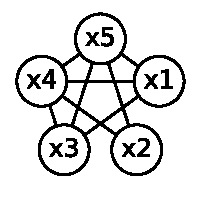
\includegraphics[width=0.625\linewidth]{img/8ec60eeeaa549478379fc4cb6b42df17c5ca8b364e4e642efbba0ac2db0b6e94.pdf}
		\vspace{-1em}
		\captionof{figure}{\centering Graf Terhubung}
		\label{fig:contoh-graf}
	\end{minipage}
	\begin{minipage}{0.4\linewidth}
		\centering
		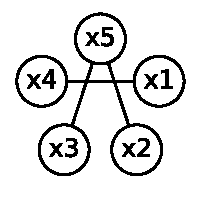
\includegraphics[width=0.625\linewidth]{img/0630ebfe671b8208b2dc56ca90c62464252c4ac5e3f30ff3fc2c6db4495f49cc.pdf}
		\vspace{-1em}
		\captionof{figure}{\centering Graf Tak Terhubung}
		\label{fig:graf-tak-terhubung}
	\end{minipage}
\end{center}

Graf terhubung adalah graf dengan setiap pasang simpulnya memiliki lintasan yang menghubungkan \citep{chartrand2000}. \autoref{fig:contoh-graf} adalah contoh graf terhubung. \autoref{fig:graf-tak-terhubung} adalah contoh graf tak terhubung karena tidak terdapat lintasan yang dapat menghubungkan \(x_1\) dan \(x_5\).

Jarak antara dua simpul \(u\) dan \(v\), dinotasikan \(d(u, v)\), adalah panjang minimum dari semua lintasan yang menghubungkan kedua simpul tersebut \citep{chartrand2000}. Panjang sebuah lintasan adalah banyaknya sisi yang membangun rangkaian lintasan tersebut. Contoh, pada \autoref{fig:contoh-graf}, nilai dari \(d(x_2, x_1)\) adalah \(2\).

Matriks ketetanggaan adalah alternatif representasi dari graf yang menunjukkan ketetanggaan, atau keberadaan sisi antar simpul \citep{west1996}. Semisalnya sebuah graf memiliki himpunan simpul \(V = \{v_1, v_2, \ldots\}\). Maka, baris dan kolom pertama dalam matriks ketetanggaannya menunjukkan \(v_1\), baris dan kolom kedua menunjukkan \(v_2\), dan seterusnya. Ketika terdapat sisi yang menghubungkan \(v_i\) ke \(v_j\), maka elemen pada baris ke-\(i\) dan kolom ke-\(j\) bernilai \(1\), sedangkan bila tidak terhubung maka bernilai \(0\). Sebagai ilustrasi, berikut adalah matriks ketetanggaan dari \autoref{fig:contoh-graf}.
\[
\left[
\begin{array}{ccccc}
	0 & 0 & 1 & 1 & 1 \\
	0 & 0 & 0 & 1 & 1 \\
	1 & 0 & 0 & 1 & 1 \\
	1 & 1 & 1 & 0 & 1 \\
	1 & 1 & 1 & 1 & 0
\end{array}
\right]
\]
Perhatikan matriks ketetanggaan simetris terhadap diagonal utama ketika graf yang direpresentasikan tak berarah.

Matriks jarak adalah matriks yang memuat jarak antara seluruh pasangan simpul \citep{chartrand2000}. Sehingga, setiap baris ke-\(i\) dan kolom ke-\(j\) berisi nilai jarak dari \(v_i\) ke \(v_j\), seperti berikut:
\[
\left[
\begin{array}{ccc}
	d(v_1, v_1) & d(v_1, v_2) & \cdots \\
	d(v_2, v_1) & d(v_2, v_2) & \cdots \\
	\vdots & \vdots & \ddots
\end{array}
\right]
\]
Sebagai gambaran, berikut adalah matriks jarak dari \autoref{fig:contoh-graf}.
\[
\left[
\begin{array}{ccccc}
	0 & 2 & 1 & 1 & 1 \\
	2 & 0 & 2 & 1 & 1 \\
	1 & 2 & 0 & 1 & 1 \\
	1 & 1 & 1 & 0 & 1 \\
	1 & 1 & 1 & 1 & 0
\end{array}
\right]
\]
Dapat diamati, setiap elemen dalam matriks jarak memiliki nilai ketika graf yang direpresentasikan adalah graf terhubung.

\section{Automorfisma Graf}

\noindent
\begin{center}
	\begin{minipage}{0.8\linewidth}
		\begin{minipage}{0.25\linewidth}
			\centering
			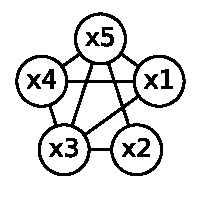
\includegraphics[width=\linewidth]{img/3637d326d230653eb5359219776827aba655cda549265e8622f29fcf4522cfb1.pdf}
			\vspace{-2em}
			\par\small (a)
		\end{minipage}
		\hfill
		\begin{minipage}{0.25\linewidth}
			\centering
			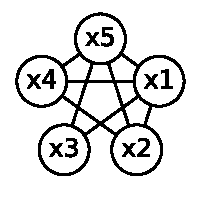
\includegraphics[width=\linewidth]{img/401a2e0bee9ea19714a37a3c2bfa4c78f5a92ea31c623ab3bc7826d5ed95c330.pdf}
			\vspace{-2em}
			\par\small (b)
		\end{minipage}
		\hfill
		\begin{minipage}{0.25\linewidth}
			\centering
			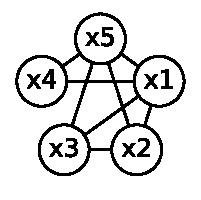
\includegraphics[width=\linewidth]{img/4b541ec99ee9b0f060e784c888fc378dca74b6d8ff80f5ccc8336615aca46695.pdf}
			\vspace{-2em}
			\par\small (c)
		\end{minipage}

		\begin{minipage}{0.25\linewidth}
			\centering
			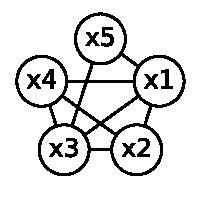
\includegraphics[width=\linewidth]{img/6eeebca324db75f7c0a719672bf306f79b5afe806b2a8814f0b2f2beedb3b891.pdf}
			\vspace{-2em}
			\par\small (d)
		\end{minipage}
		\hfill
		\begin{minipage}{0.25\linewidth}
			\centering
			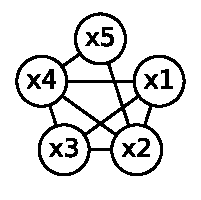
\includegraphics[width=\linewidth]{img/71f4c81555ee6516f44f4d05f5e6f67edd5de0ed42a1cdbcb2f2af72c3232b75.pdf}
			\vspace{-2em}
			\par\small (e)
		\end{minipage}
		\hfill
		\begin{minipage}{0.25\linewidth}
			\centering
			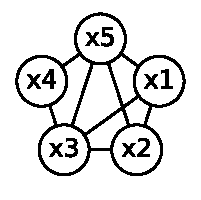
\includegraphics[width=\linewidth]{img/7d7c7231a399fc001d20da820222d60b8205b145c0e4fafd9cf2f3ebf1eec22d.pdf}
			\vspace{-2em}
			\par\small (f)
		\end{minipage}
		\captionof{figure}{Automorfisma Graf}
		\label{fig:contoh-automorfisma}
	\end{minipage}
\end{center}

Automorfisma graf adalah isomorfima suatu graf ke dirinya sendiri. Salah satu cara untuk menunjukkan automorfisma graf adalah menggunakan representasi kanonik. Hal ini telah dilakukan oleh \citeauthor{mckay2014} di \citeyear{mckay2014}. Jika dua graf memiliki representasi kanonik yang sama, maka kedua graf tersebut isomorfik. Sebaliknya, jika representasi kanonik berbeda, maka kedua graf tersebut tidak isomorfik.

Untuk graf tak berarah, representasi kanonik oleh \citeauthor{mckay2014} dituliskan dalam format \verb`graph6`. Sebagai ilustrasi, \autoref{fig:contoh-graf} memiliki representasi \verb`DV{` dalam format \verb`graph6`. Kemudian, setiap graf pada \autoref{fig:contoh-automorfisma}, dari (a) sampai (f), berturut-turut memiliki representasi \verb`D\{`, \verb`Du{`,  \verb`D{{`,  \verb`D~g`,  \verb`D~S`,  dan \verb`Dx{` dalam format \verb`graph6`. Akan tetapi, graf pada \autoref{fig:contoh-graf} dan semua graf pada \autoref{fig:contoh-automorfisma} memiliki representasi kanonik yang sama, yaitu \verb`DN{` dalam format \verb`graph6`, sehingga semuanya merupakan automorfisma dari graf yang sama.

\section{Dimensi Metrik}

Misalkan \(G\) adalah sebuah graf terhubung dengan himpunan simpul \(V = \{v_1, v_2, \ldots, v_n\}\), dan \(d(x, y)\) adalah jarak antara simpul \(x\) dan \(y\) di \(G\). Pilih sembarang \(W = \{w_1, w_2, \ldots, w_k\} \subseteq V\). Untuk \(v \in V\), tupel terurut
	\[ r(v|W) = (d(w_1, v), d(w_2, v), \ldots, d(w_k, v)) \]
adalah representasi dari \(v\) terhadap \(W\). Himpunan \(W\) adalah \foreign{resolving set}, atau himpunan pembeda, untuk \(G\) apabila
	\[ \forall u, v \in V, u \neq v \implies r(u|W) \neq r(v|W) \]
atau dengan kata lain, seluruh simpul dalam \(G\) memiliki representasi unik terhadap \(W\).

Dimensi metrik dari \(G\) adalah kardinalitas minimum dari himpunan pembeda untuk \(G\) \citep{tillquist2023}. Sebagai ilustrasi, untuk graf pada \autoref{fig:contoh-graf}, jika dipilih \(W = \{x_2, x_4\}\), akan diperoleh representasi terhadap \(W\) berikut:
\[
\begin{array}{c@{\ }c@{\ }c@{\ }c@{\ }c}
	r(x_1|W) & = & ( d(x_2, x_1), \; d(x_4, x_1) ) & = & (2, 1) \\
	r(x_2|W) & = & ( d(x_2, x_2), \; d(x_4, x_2) ) & = & (0, 1) \\
	r(x_3|W) & = & ( d(x_2, x_3), \; d(x_4, x_3) ) & = & (2, 1) \\
	r(x_4|W) & = & ( d(x_2, x_4), \; d(x_4, x_4) ) & = & (1, 0) \\
	r(x_5|W) & = & ( d(x_2, x_5), \; d(x_4, x_5) ) & = & (1, 1)
\end{array}
\]
Ditemukan \(\{x_2, x_4\}\) bukanlah himpunan pembeda karena \(r(x_1|W) = r(x_3|W)\). Untuk \autoref{fig:contoh-graf}, tidak ada himpunan pembeda dengan kardinalitas 2. Dimensi metrik dari graf ini adalah 3, dengan contoh solusi \(\{x_1, x_4, x_5\}\), atau \(\{x_1, x_3, x_4\}\), dan himpunan pembeda lainnya yang berkardinalitas 3.

\section{Dimensi Metrik Sisi}

Misalkan \(G\) adalah sebuah graf terhubung dengan himpunan simpul \(V\), himpunan sisi \(E = \{e_1, e_2, \ldots, e_n\}\), dan \(d(x, y)\) adalah jarak antara simpul \(x\) dan \(y\) di \(G\). Untuk sembarang simpul \(z\) dan sembarang sisi \(e\) di \(G\), jika \(e\) adalah sisi yang menghubungkan simpul \(x\) dan \(y\), maka jarak dari \(z\) ke \(e\) adalah \( d(z, e) = \min(d(z, x), d(z, y)) \). Ambil sembarang \(W = \{w_1, w_2, \ldots, w_k\} \subseteq V\). Untuk \(e \in E\), tupel terurut
	\[ r(e|W) = (d(w_1, e), d(w_2, e), \ldots, d(w_k, e)) \]
adalah representasi dari \(e\) terhadap \(W\). Himpunan \(W\) adalah \foreign{edge resolving set}, atau himpunan pembeda sisi, untuk \(G\) apabila
	\[ \forall e, f \in E, e \neq f \implies r(e|W) \neq r(f|W) \]
atau dengan kata lain, seluruh sisi dalam \(G\) memiliki representasi unik terhadap \(W\).

Dimensi metrik sisi dari \(G\) adalah kardinalitas minimum dari himpunan pembeda sisi untuk \(G\) \citep{kelenc2018}. Sebagai ilustrasi, untuk graf pada \autoref{fig:contoh-graf}, jika dipilih \(W = \{x_1, x_4, x_5\}\), akan diperoleh representasi terhadap \(W\) berikut:
\[
\begin{array}{c@{\ }c@{\ }c@{\ }c@{\ }c}
	r(e_1|W) & = & ( d(x_1, e_1), \; d(x_4, e_1), \; d(x_5, e_1) ) & = & (0, 1, 1) \\
	r(e_2|W) & = & ( d(x_1, e_2), \; d(x_4, e_2), \; d(x_5, e_2) ) & = & (0, 0, 1) \\
	r(e_3|W) & = & ( d(x_1, e_3), \; d(x_4, e_3), \; d(x_5, e_3) ) & = & (0, 1, 0) \\
	r(e_4|W) & = & ( d(x_1, e_4), \; d(x_4, e_4), \; d(x_5, e_4) ) & = & (1, 0, 1) \\
	r(e_5|W) & = & ( d(x_1, e_5), \; d(x_4, e_5), \; d(x_5, e_5) ) & = & (1, 1, 0) \\
	r(e_6|W) & = & ( d(x_1, e_6), \; d(x_4, e_6), \; d(x_5, e_6) ) & = & (1, 0, 1) \\
	r(e_7|W) & = & ( d(x_1, e_7), \; d(x_4, e_7), \; d(x_5, e_7) ) & = & (1, 1, 0) \\
	r(e_8|W) & = & ( d(x_1, e_8), \; d(x_4, e_8), \; d(x_5, e_8) ) & = & (1, 0, 0)
\end{array}
\]
Ditemukan \(\{x_1, x_4, x_5\}\) bukanlah himpunan pembeda sisi karena \(r(e_4|W) = r(e_6|W)\). Untuk \autoref{fig:contoh-graf}, tidak ada himpunan pembeda sisi dengan kardinalitas 3. Dimensi metrik sisi dari graf ini adalah 4, dengan contoh solusi \(\{x_1, x_2, x_3, x_4\}\), atau \(\{x_1, x_2, x_3, x_5\}\), dan himpunan pembeda sisi lainnya yang berkardinalitas 4.

\section{\foreign{Satisfiability Modulo Theories}}

SMT, atau \foreign{satisfiability modulo theories}, secara umum adalah proses mencari nilai dari variabel-variabel dalam ekspresi matematika yang menyebabkan ekspresi tersebut menjadi benar. Jika suatu solusi ada, ekspresi tersebut terbilang \foreign{satisfiable}. Jika solusi tidak ada, ekspresi tersebut terbilang \foreign{unsatisfiable}. Proses ini tidak menentukan solusi mana yang akan diberikan, melainkan hanya mencari satu solusi apa pun, yang kemudian disebut sebagai \foreign{model}.

Istilah \foreign{modulo theories} merujuk pada penggunaan teori tertentu, seperti aritmetika bilangan bulat, bilangan riil, \foreign{array}, atau \foreign{bit-vectors}. Pemilihan teori biasanya disesuaikan dengan tujuan pemodelan. Bergantung pada apakah suatu permasalahan ingin ditunjukkan sebagai \foreign{satisfiable} atau \foreign{unsatisfiable}, teori yang digunakan dapat pula berbeda untuk memfasilitasi pemanfaatan sifat-sifat permasalahan tersebut agar lebih ramah terhadap komputasi.

\foreign{Solver} adalah program yang mengimplementasikan proses dari SMT, mengevaluasi ekspresi, dan dapat menghasilkan \foreign{model}. Secara komputasi, \foreign{solver} mungkin saja tidak menghasilkan hasil, karena hal-hal seperti konfigurasi batas waktu eksekusi, atau keterbatasan implementasi untuk beberapa teori. Penjelasan lebih lengkap mengenai SMT dapat ditemukan pada \cite{barrett2018}.

Terdapat berbagai macam \foreign{solver} SMT, baik yang bersifat \foreign{general-purpose} maupun yang \foreign{special-purpose} untuk jenis \foreign{constraint} atau teori tertentu. Sebagai contoh, sistem persamaan linear dapat dimodelkan dalam teori \foreign{linear real arithmetic}, yang umumnya dapat diselesaikan oleh \foreign{general-purpose solver}. Di sisi lain, kelas permasalahan seperti sistem non-linier atas \foreign{integer} --- juga dikenal sebagai \foreign{Hilbert's Tenth Problem}, yang telah dibuktikan \foreign{undecidable} secara umum \citep{matiiaasevich1993} --- memerlukan \foreign{special-purpose solver}; seperti penelitian yang telah dilakukan oleh \cite{nuzzo2010} atau \cite{borralleras2020} yang menargetkan \foreign{subset} tertentu dari permasalahan tersebut dan mengeksploitasi sifat khusus seperti konveksitas, maupun teknik tertentu seperti linearisasi.

\subsection{\foreign{Boolean Satisfiability}}

\foreign{Boolean satisfiability} dalam SMT adalah teori yang memuat variabel boolean dan operasi boolean pada umumnya \citep{yurichev}. Sebagai ilustrasi, dapat diperhatikan ekspresi \((x_1 \land x_2) \lor (x_1 \land x_3)\) dengan \(x_1, x_2, x_3\) adalah variabel boolean. Tabel kebenaran untuk ekspresi tersebut dapat dikonstruksi seperti berikut:
\vspace{-0.5em}
\[
\begin{array}{cccc}
	x_1 & x_2 & x_3 & (x_1 \land x_2) \lor (x_1 \land x_3) \\ [4pt]
	\False & \False & \False & \False \\
	 \True & \False & \False & \False \\
	\False &  \True & \False & \False \\
	 \True &  \True & \False &  \True \\
	\False & \False &  \True & \False \\
	 \True & \False &  \True &  \True \\
	\False &  \True &  \True & \False \\
	 \True &  \True &  \True &  \True
\end{array}
\]

\noindent Oleh karena itu, salah satu \foreign{model} yang dapat dihasilkan oleh \foreign{solver} adalah \(x_1 = \True, x_2 = \False, x_3 = \True\).

Dalam \foreign{boolean satisfiability}, terdapat pula batasan \(\mathrm{AtLeast}\) dan \(\mathrm{AtMost}\) untuk menentukan paling sedikit dan paling banyak variabel yang boleh bernilai benar. Misalnya, dengan menambahkan batasan \(\mathrm{AtLeast}(3)\) ke contoh sebelumnya, \(x_1 = \True, x_2 = \False, x_3 = \True\) tidaklah lagi solusi yang sah.

\subsection{\foreign{Pseudo Boolean}}

\foreign{Pseudo boolean} adalah ekstensi dari teori \foreign{boolean satisfiability} yang dapat menyatakan bentuk ekspresi linear dengan koefisien bilangan bulat atas variabel boolean \citep{yurichev}. Teori ini mendukung tiga operasi relasi, yaitu:
\[
\begin{array}{lcl}
	a_1 x_1 + a_2 x_2 + \ldots + a_i x_i &\leq& a \\
	b_1 x_1 + b_2 x_2 + \ldots + b_j x_j &=& b \\
	c_1 x_1 + c_2 x_2 + \ldots + c_k x_k &\geq& c \\
\end{array}
\]
di mana \(a, a_1, \ldots, a_i, b, b_1, \ldots, b_j, c, c_1, \ldots, c_k\) adalah konstanta \foreign{integer} (bilangan bulat), dan \(x_1,\ldots,x_i,x_j,x_k\) adalah variabel boolean. Ketika variabel boolean bernilai benar, perkaliannya dengan konstanta menjadi seperti perkalian dengan angka 1. Ketika variabel boolean bernilai salah, perkaliannya dengan konstanta menjadi seperti perkalian dengan angka 0. Ambil contoh berikut:
\[
\begin{array}{rcl}
	x_1 + x_2 + x_3 + x_4 &=& 2 \\
	x_1 + x_2 &\leq& 1 \\
	x_3 + x_4 &\leq& 1
\end{array}
\]
dengan \(x_1, x_2, x_3, x_4\) adalah variabel boolean. Ekspresi ini memiliki seluruh konstantanya yang sama dengan 1. Salah satu \foreign{model} yang dapat dihasilkan oleh \foreign{solver} adalah \(x_1 = \True, x_2 = \False, x_3 = \True, x_4 = \False\).

\subsection{\foreign{Linear Integer Arithmetic}}

\foreign{Linear integer arithmetic}, atau LIA, dalam SMT adalah teori yang memuat variabel \foreign{integer}, atau bilangan bulat, dan operasi \foreign{integer} pada umumnya \citep{yurichev}. Contoh \foreign{pseudo boolean} sebelumnya dapat dinyatakan ulang dalam bentuk LIA.
\[
\begin{array}{rcl}
	x_1 + x_2 + x_3 + x_4 &=& 2 \\
	x_1 + x_2 &\leq& 1 \\
	x_3 + x_4 &\leq& 1
\end{array}
\]
\[ 0 \leq x_1 \leq 1, \quad 0 \leq x_2 \leq 1, \quad 0 \leq x_3 \leq 1, \quad 0 \leq x_4 \leq 1 \]
dengan \(x_1, x_2, x_3, x_4\) adalah variabel \foreign{integer}. \foreign{Model} yang dapat dihasilkan oleh \foreign{solver} yang mirip dengan hasil dari \foreign{pseudo boolean} sebelumnya adalah \(x_1 = 1, x_2 = 0, x_3 = 1, x_4 = 0\).

\section{Z3}

Z3 adalah salah satu dari banyak \foreign{solver} SMT yang ada. Z3 dikembangkan oleh Microsoft Research dan dirancang khusus untuk menyelesaikan formula logika dari berbagai macam jenis teori. Z3 merupakan \foreign{solver} modular, dengan menggunakan arsitektur DPLL(T), menggabungkan berbagai prosedur untuk teori-teori yang berbeda \citep{demoura2008}.

Dibandingkan dengan \foreign{solver} lain yang hanya mengkhususkan diri pada teori-teori tertentu, Z3 mendukung kombinasi teori yang lebih kompleks . Selain itu, Z3 juga mendukung penyelesaian inkremental, generasi bukti (\foreign{proof generation}), ekstraksi \foreign{unsat core}, serta penggunaan kuantor (universal dan eksistensial) \citep{bjorner}.

Perlu dipahami bahwa Z3, maupun SMT \foreign{solver} pada umumnya, tidak melakukan manipulasi simbolik sebagaimana \foreign{computer algebra system} (CAS). SMT \foreign{solver} difokuskan pada penentuan \foreign{satifiability} suatu ekspresi menggunakan prosedur seperti DPLL(T) \citep{demoura2008, bjorner}. Sebaliknya, CAS dirancang untuk manipulasi simbolik seperti penyederhanaan ekspresi, integrasi, atau diferensiasi simbolik \citep{geddes1992}. Oleh karena itu, SMT \foreign{solver} dan CAS merupakan kelas asisten komputasi yang berbeda.

	\cleardoublepage

	\newcommand{\mcol}[3]{\multicolumn{#1}{#2}{#3}}
\newcommand{\mrow}[2]{\multirow{#1}{*}{#2}}
\newcommand{\cellb}{\cellcolor[HTML]{000000}}

\chapter{Metodologi}

Metodologi yang digunakan dalam tugas akhir ini dirancang untuk menyusun, mengimplementasikan, dan mengevaluasi pendekatan berbasis SMT dalam menghitung dimensi metrik dan dimensi metrik sisi suatu graf. Tahapan metodologi ini dibagi menjadi beberapa bagian sebagaimana diilustrasikan oleh \autoref{fig:diagram-alir}.

\begin{figure}[!htbp]
	\centering
	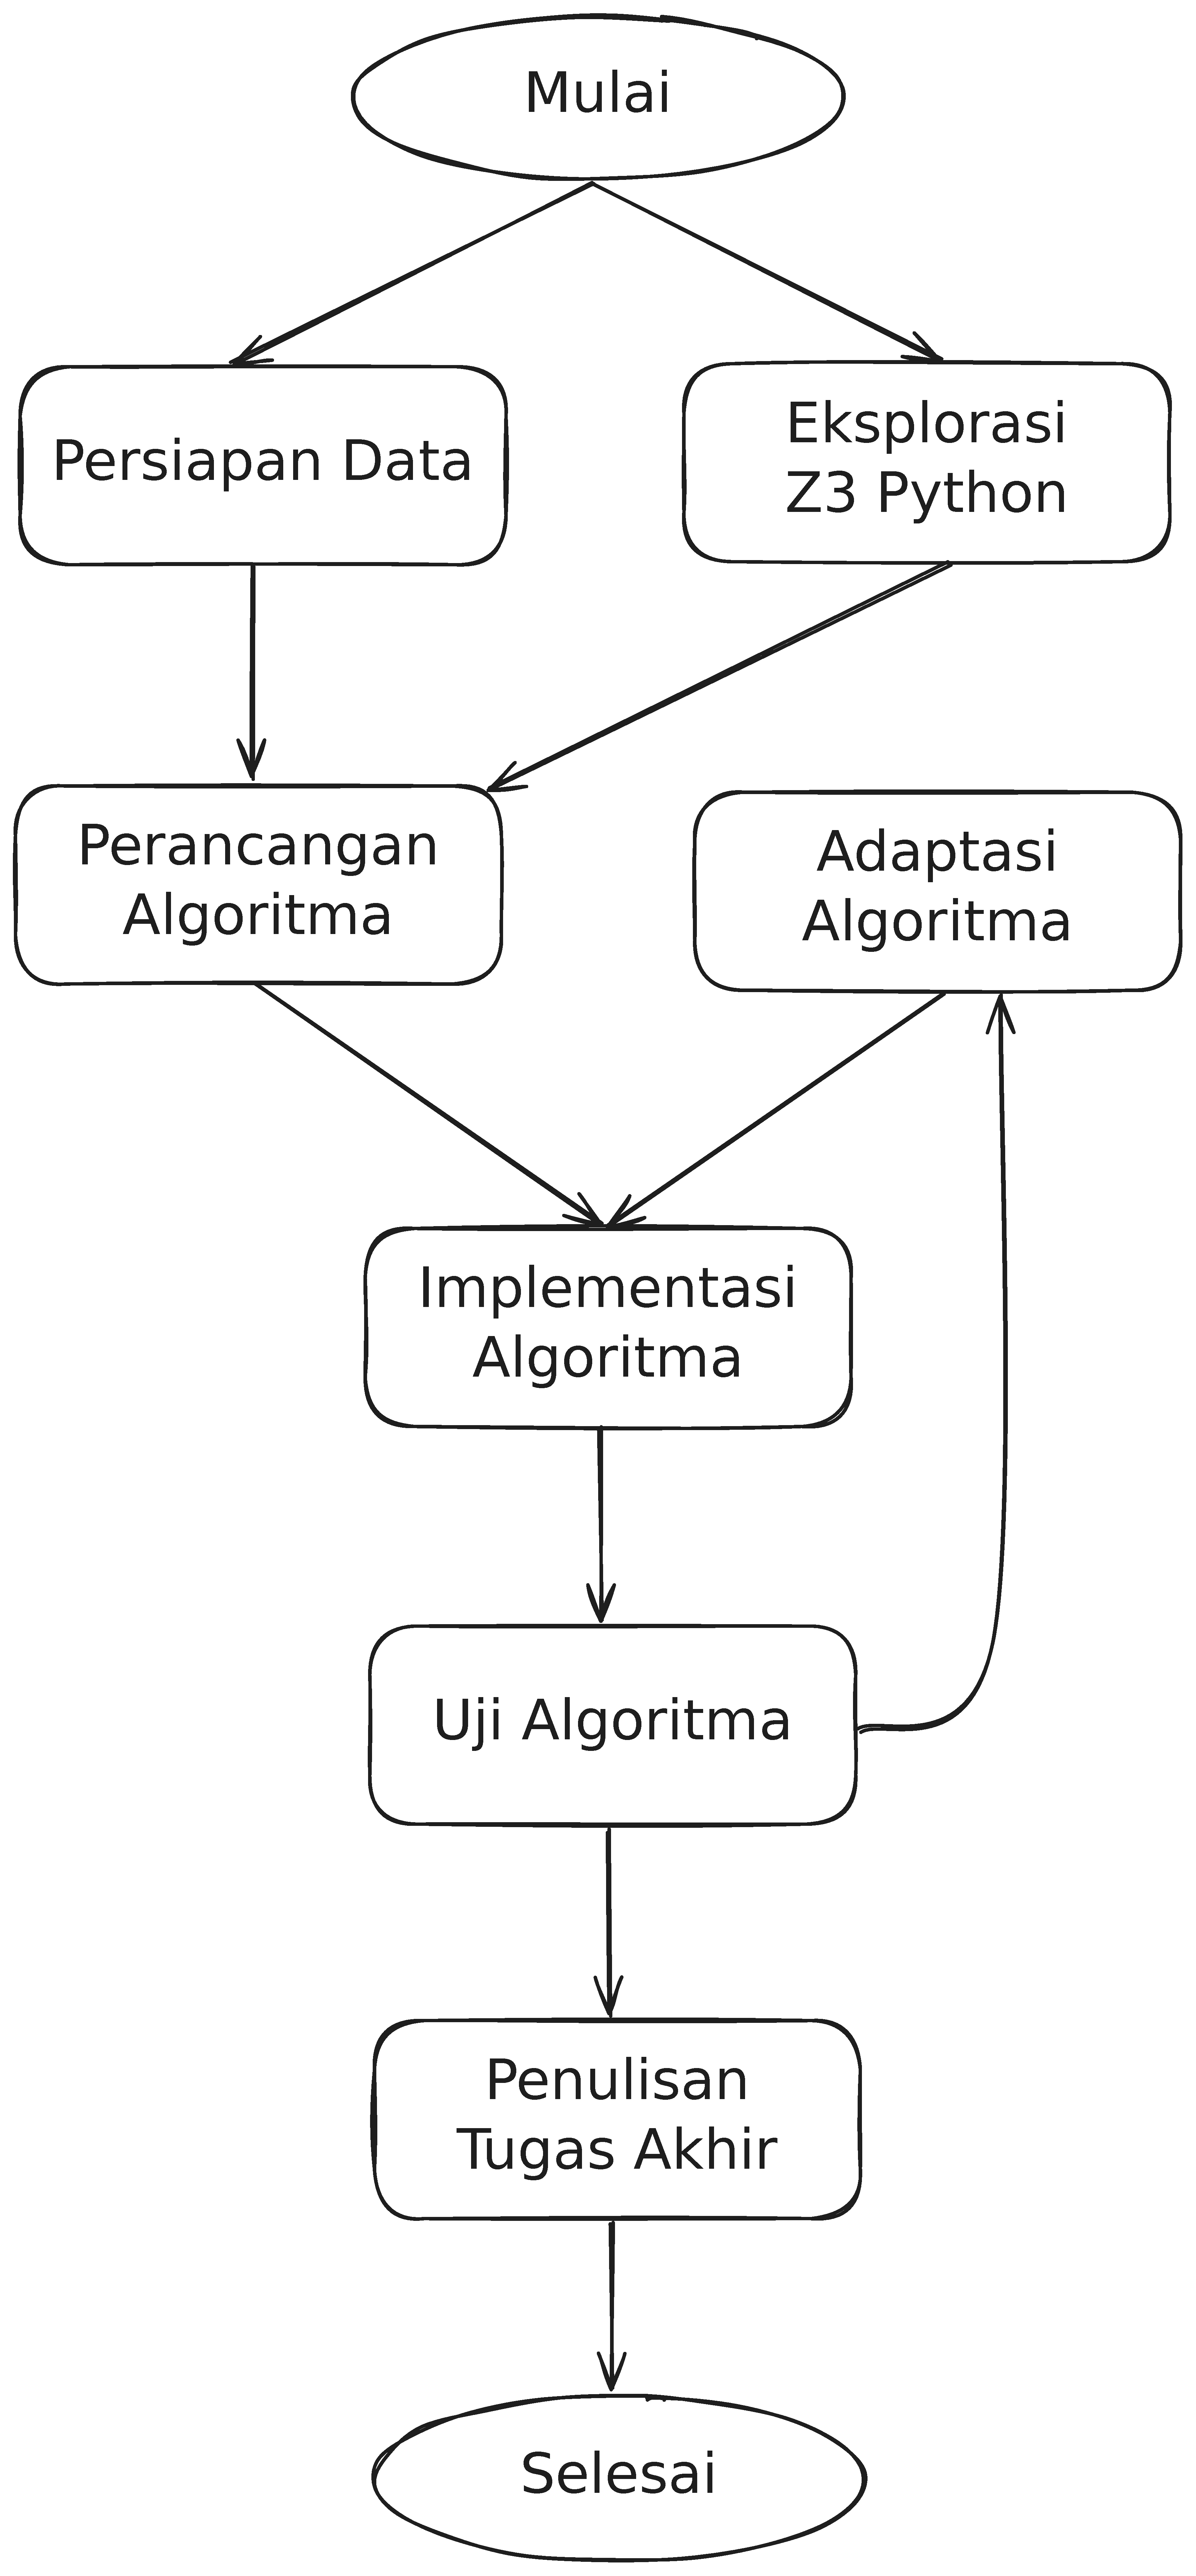
\includegraphics[width=0.5\linewidth]{img/diagram-alir-metodologi.pdf}
	\caption{Diagram Alir Metodologi}
	\label{fig:diagram-alir}
\end{figure}

\clearpage
\section{Persiapan Data}
\label{sec:data}

Data graf yang digunakan dibagi menjadi dua kategori: graf kecil (2 hingga 9 simpul) dan graf besar (lebih dari 9 simpul).

\begin{enumerate}

	\item Graf Kecil

	Graf tak berarah dengan banyak simpul 2 hingga 9 digenerasikan menggunakan program \verb`nauty-geng`. Program ini menghasilkan seluruh graf dengan banyak simpul yang dispesifikasikan dan juga mengeliminasi semua redundansi automorfimanya. Opsi \verb`-c` diberikan kepada program untuk memastikan hanya graf terhubung yang dihasilkan.

	\item Graf Besar

	Graf besar digenerasikan secara acak menggunakan program \verb`nauty-genrang`. Opsi \verb`-g` diberikan kepada program untuk memastikan hanya graf tak berarah yang dihasilkan. Untuk menghindari duplikasi akibat automorfisma, setiap graf diproses menggunakan program \verb`nauty-labelg` untuk menghasilkan representasi kanonik. Kemudian, program \verb`nauty-pickg` dengan opsi \verb`-vc0` digunakan untuk memilih hanya graf yang terkoneksi.

\end{enumerate}

Semua graf disimpan dalam \foreign{file} teks menggunakan format \verb`graph6`. Graf dengan banyak simpul yang sama disimpan dalam file yang sama. Banyak simpul maksimum yang dapat diuji bergantung pada keterbatasan waktu dan sumber daya komputasi yang tersedia.

\section{Eksplorasi Z3 Python}

Pada tahap ini dilakukan eksplorasi SMT \foreign{solver}, yaitu Z3, menggunakan \foreign{binding} untuk bahasa Python. Aktivitas meliputi:

\begin{enumerate}

	\item Mempelajari fitur dasar Z3 yang relevan dengan formulasi masalah kombinatorial pada teori graf.

	\item Mencoba contoh sederhana untuk memahami cara mendefinisikan variabel, batasan (\foreign{constraints}), serta strategi pencarian solusi.

	\item Mengevaluasi kemampuan Z3 dalam menangani permasalahan berukuran kecil maupun besar untuk mengidentifikasi potensi kendala performa.

\end{enumerate}

\section{Perancangan Algoritma}

Perancangan algoritma difokuskan pada formulasi masalah dimensi metrik ke dalam bentuk SMT. Pertama, graf direpresentasikan dalam bentuk matriks ketetanggaan yang dibaca dari format \verb`graph6`. Kedua, matriks jarak dapat dibangun dari matriks ketetanggaan menggunakan algoritma \foreign{Floyd–Warshall}. Kemudian, berdasarkan dua informasi ini, dirancanglah algoritma yang memetakan pencarian dimensi metrik ke dalam bentuk batasan yang dapat dicerna oleh SMT.

Dalam tugas akhir ini, digunakan tiga teori dalam SMT, yaitu \foreign{boolean satisfiability}, \foreign{pseudo boolean}, dan \foreign{linear integer arithmetic}. Dipilih teori \foreign{boolean satisfiability} karena permasalahan dimensi metrik yang perlu memodelkan \foreign{resolving set}, yaitu memilih keanggotaan simpul graf yang dapat dinyatakan menggunakan \foreign{constraints} boolean. Sedangkan teori \foreign{pseudo boolean} serta \foreign{linear integer arithmetic} dipilih sebagai eksplorasi tambahan mengenai kapabilitas SMT, karena translasi \foreign{constraint} dari \foreign{boolean satisfiability} ke dalam kedua teori ini yang masih cukup mudah untuk dilakukan.

\section{Implementasi Algoritma}

Algoritma yang telah dirancang kemudian diimplementasikan ke bentuk kode. Hal-hal yang perlu dilakukan diantaranya adalah:

\begin{enumerate}

		\item Pembacaan graf dari \foreign{file} teks \verb`graph6`.

		\item Formulasi batasan untuk SMT dari informasi graf.

		\item Eksekusi Z3 \foreign{solver} dan dapatkan dimensi metrik.

		\item Simpan hasil perhitungan ke dalam \foreign{file} teks untuk analisis lebih lanjut.

\end{enumerate}

\section{Uji Algoritma}

Pengujian dilakukan secara bertahap untuk memverifikasi kebenaran implementasi serta mengevaluasi kinerjanya.

\begin{enumerate}

	\item{Uji pada Sampel Kecil}

	Beberapa graf kecil dipilih sebagai sampel. Tujuan tahap pengujian ini adalah memverifikasi bahwa rancangan algoritma dan implementasi program menghasilkan solusi yang benar.

	\item{Uji pada Seluruh Graf Kecil}

	Seluruh graf terhubung dengan 2–9 simpul diuji secara menyeluruh. Tujuan tahap pengujian ini adalah untuk mendapatkan data komprehensif kinerja algoritma dengan berbagai macam konfigurasi graf. Data ini dapat dianalisis kasus-kasusnya seperti kejadian \foreign{worst-case} dan kejadian \foreign{best-case}. Hasil ini juga dapat dibandingkan dengan literatur yang ada untuk validasi.

	\item{Uji pada Graf Besar}

	Pengujian diperluas pada graf dengan simpul lebih banyak. Tujuan tahap pengujian ini adalah mengevaluasi kinerja dan keterbatasan pendekatan SMT pada kasus yang lebih kompleks. Uji ini juga yang dijadikan sebagai tolak ukur performa solusi dari tugas akhir ini secara umum untuk sembarang graf.

\end{enumerate}

\section{Adaptasi Algoritma}

Tahap adaptasi dilakukan dengan memodifikasi algoritma yang telah ada untuk menghitung dimensi metrik sisi. Proses adaptasi mencakup:

\begin{enumerate}

	\item Menyesuaikan representasi graf sehingga memperhatikan jarak antar sisi.

	\item Memformulasikan kembali permasalahan ke dalam SMT.

	\item Mengimplementasikan kembali ke bentuk kode.

	\item Mengulangi tahapan pengujian: mulai dari sampel kecil, seluruh graf kecil, hingga graf besar.

\end{enumerate}

\section{Penulisan Tugas Akhir}

Tahap terakhir dari metodologi ini adalah penyusunan seluruh hasil penelitian ke dalam bentuk laporan tugas akhir. Penulisan dilakukan sesuai pedoman akademik yang berlaku sehingga hasil penelitian terdokumentasi dengan baik dan dapat dijadikan rujukan untuk penelitian selanjutnya.

	\cleardoublepage

	\chapter{Hasil dan Pembahasan}
\newcommand{\combine}[7]{#1 #2 \vphantom{#6} #3 #4 #5 #6 \vphantom{#2} #7}

\newcommand{\minipagealign}{}
\newcommand{\minipagewidth}{\linewidth}

\newlength{\contentwidth}
\newcommand{\resizetofit}[1]{
	\settowidth{\contentwidth}{#1}
	\ifdim\contentwidth > \linewidth
		\resizebox{\linewidth}{!}{#1}
	\else
		#1
	\fi
}

\section{Landasan Formal}

Untuk mempermudah pembahasan, terlebih dahulu didefinisikan beberapa notasi. Misalkan \(S\) merupakan suatu himpunan sembarang. Sebuah vektor berdimensi \(n\) yang elemennya berasal dari \(S\) ditulis sebagai \(c \in S^n\), dengan \(c_i \in S\) menyatakan elemen ke-\(i\) dari vektor tersebut. Vektor \(c\) dapat dibangun dari elemen-elemennya dengan notasi \(c = (c_1\ \cdots\ c_n)\), atau secara singkat \(c = (c_i\ \cdots)\) ketika domain indeks \(i\) jelas dari konteks.

Selanjutnya, sebuah matriks \(A\) berukuran \(m\) baris dan \(n\) kolom yang elemennya berasal dari \(S\) ditulis sebagai \(A \in S^{m\times n}\), dengan \(A_{ij} \in S\) menyatakan elemen di baris ke-\(i\) dan kolom ke-\(j\) dari matriks tersebut. Digunakan notasi \(A_{*j} \in S^m\) untuk kolom ke-\(j\) dan notasi \(A_{i*} \in S^n\) untuk baris ke-\(i\).

Kemudian, misalnya, diberikan \(a_1,\ \cdots,\ a_m \in S^n\). Sebuah matriks \(A \in S^{n\times m}\) dapat dibangun dengan menyusun vektor-vektor tersebut secara bersampingan, yaitu \(A = [a_1\ \cdots\ a_m]\), atau secara singkat \(A = [a_i\ \cdots]\) ketika domain indeks \(i\) jelas dari konteks. Dan sebuah matriks \(A \in S^{m\times n}\) dapat dibangun dengan menyusun vektor-vektor tersebut secara bertumpuk, yaitu
	\[ A = \left[ \begin{array}{c} a_1\\ \vdots\\ a_m \end{array} \right], \quad \text{atau secara singkat } A = \left[ \begin{array}{c} a_i\\ \vdots \end{array} \right] \text{.}\]

Dengan demikian, matriks \(A\) dapat dibangun dari elemen-elemen barisnya maupun dari elemen-elemen kolomnya sebagai berikut.
	\[ A = \left[ \begin{array}{c} A_{i*}\\ \vdots \end{array} \right] = [A_{*j}\ \cdots] \]

Didefinisikan dua operator biner, yaitu \((s_1 = s_2)\) dan \((t_1 | t_2)\), serta satu operator unari, yaitu \((\sim\!t)\), yang memetakan unsur-unsurnya kepada nilai boolean \(\Bbb = \{\True, \False\}\), untuk sembarang \(s_1, s_2 \in S\) serta \(t, t_1, t_2 \in \Bbb\).
\[
\begin{array}{r@{\ }l}
	(s_1 = s_2) &= \left\{
		\begin{array}{l@{\ }l}
			\True  &\iff s_1 = s_2 \\
			\False &\iff s_1 \neq s_2
		\end{array} \right. \\ [16pt]
	(s_1 | s_2) &= \left\{
		\begin{array}{l@{\ }l@{\ }c}
			\True  &\iff& s_1 \vee s_2 \\
			\False &\iff& \neg s_1 \wedge \neg s_2
		\end{array} \right. \\ [16pt]
	(\sim\!s) &= \left\{
		\begin{array}{l@{\ }l@{\ }c}
			\True  &\iff& \neg s \\
			\False &\iff& s
		\end{array} \right.
\end{array}
\]
Secara natural, setiap operator tersebut dapat diperluas untuk unsur-unsur vektor yang dipetakan ke \(\Bbb^n\). Apabila \(a, b \in S^n\), maka \((a = b) = ((a_i = b_i)\ \cdots)\). Sedangkan untuk \(\alpha, \beta \in \Bbb^n\), maka \((\alpha | \beta) = ((\alpha_i | \beta_i)\ \cdots)\) dan juga \((\sim\!\alpha) = ((\sim\!\alpha_i)\ \cdots)\).

Terakhir, diperkenalkan beberapa notasi yang berhubungan dengan graf. Misalkan \(G\) adalah graf. Representasi graf \(G\) dalam bentuk matriks ketetanggaan ditulis sebagai \(M\). Untuk \(V\), himpunan seluruh simpul di \(G\), matriks jarak simpul ke simpul dari \(G\) ditulis sebagai \(D^{(V)}\), sehingga jarak antar dua simpul \(v_i,u_j \in V\) adalah \(d(v_i,u_j) = D^{(V)}_{ij}\). Untuk \(E\), himpunan seluruh sisi di \(G\), matriks jarak simpul ke sisi dari \(G\) ditulis sebagai \(D^{(E)}\), sehingga jarak antara simpul \(v_i \in V\) dan sisi \(e_j \in E\) adalah \(d(v_i,e_j) = D^{(E)}_{ij}\).


\section{Formulasi Algoritma}
\label{sec:alg}

Pondasi yang digunakan oleh seluruh formulasi algoritma di sini adalah matriks yang bernama \foreign{reduced distance similarity matrix} untuk penentuan dimensi metrik, atau \foreign{reduced edge distance similarity matrix} untuk dimensi metrik sisi. Untuk membangun masing-masing matriks tersebut, diperlukan matriks jarak simpul ke simpul dan matriks jarak simpul ke sisi.

Oleh karena itu, \foreign{input} yang digunakan adalah representasi matriks ketetanggaan \(M\) dari graf \(G\). Kemudian, \(D^{(V)}\) dapat dikonstruksi menggunakan algoritma \foreign{Floyd-Warshall} \citep{floyd1962, warshall1962} dari \(M\) dengan mudah. Sementara \(D^{(E)}\) dapat dikonstruksi langsung dari definisi jarak simpul ke sisi; yaitu jarak dari simpul \(v_i \in V\) ke sisi \(e_j \in E\), di mana \(e_j\) adalah sisi yang menghubungkan dua simpul \(v_k, v_l \in V\), adalah \(d(v_i,e_j) = \min(d(v_i, v_k), d(v_i, v_l))\), sehingga \(D^{(E)}_{ij} = \min(D^{(V)}_{ik}, D^{(V)}_{il})\).

\foreign{Distance similarity matrix} dari \(G\) yang dinotasikan \(B^{(V)} \in \Bbb^{|V|\times \frac{(|V|-1)|V|}{2}}\) dan \foreign{edge distance similarity matrix} dari \(G\) yang dinotasikan \(B^{(E)} \in \Bbb^{|V|\times \frac{(|E|-1)|E|}{2}}\) berturut-turut merupakan hasil dari perbandingan antara setiap kolom berbeda di \(D^{(V)}\) dan \(D^{(E)}\).
	\[ B^{(V)} = [(D^{(V)}_{*j} = D^{(V)}_{*k})\ \cdots], \quad j < k\]
	\[ B^{(E)} = [(D^{(E)}_{*j} = D^{(E)}_{*k})\ \cdots], \quad j < k\]

Kemudian, dari \(B^{(V)}\), dikonstruksi matriks yang bernama \foreign{reduced distance similarity matrix}, dan dinotasikan \(P^{(V)}\), atau dari \(B^{(E)}\), dikonstruksi matriks yang bernama \foreign{reduced edge distance similarity matrix}, dan dinotasikan \(P^{(E)}\), menggunakan algoritma berikut.
\begin{enumerate}
	\item Tetapkan \(P := B\).
	\item Untuk setiap \(P_{*j}\) dan \(P_{*k}\) dan \(j \neq k\), hapus \(P_{*j}\) jika \((P_{*j} | P_{*k}) = P_{*k}\).
\end{enumerate}

Seluruh formulasi algoritma yang akan datang didasari dari interpretasi \(P^{(V)}\) maupun \(P^{(E)}\). Maka dari itu, dibahas terlebih dahulu pemaknaan informasi yang dikandung oleh \(P\).

Pertama-tama, dapat diamati hubungan antara jarak dan representasi. Secara definisi, representasi dibangun dari jarak, yaitu \(r(\cdot|V)=(d(v_i,\cdot)\ \cdots)\). Artinya, jarak dapat diambil tarbalik dari representasi sebagai \(d(v_i,\cdot) = r_i(\cdot|V)\) untuk \(v_i \in V\). Dengan begitu, untuk \(W \subseteq V\), representasi terhadapt \(W\) dapat diambil langsung dari representasi terhadap \(V\) dengan cara \(r(\cdot|W) = (r_i(\cdot|V)\ \cdots), w_i \in W\).

Kedua, dapat dicermati hubungan antara matriks jarak dan representasi. Matriks jarak dapat dibangun dari representasi sebagai kolom-kolomnya, yaitu \(D = [r(\cdot_j|V)\ \cdots]\). Sebaliknya, representasi dapat diambil langsung dari kolom matriks jarak sebagai \(r(\cdot_j|V) = D_{*j}\). Sehingga, representasi terhadap sembarang \(W \subseteq V\) sudah termuat dalam matriks jarak, dan dapat diambil menggunakan dua bentuk pendekatan.
\begin{enumerate}
	\item Ambil kolom kemudian baris:
		\(
		\begin{array}{r@{}c@{\ }l}
			r(\cdot_j|W) = (&(D_{*j})_i&\ \cdots) \\
			= (&D_{ij}&\ \cdots) \quad, w_i \in W
		\end{array}
		\)
	\item Ambil baris kemudian kolom:
		\, \( r(\cdot_j|W) = \left[ \begin{array}{c} D_{i*}\\ \vdots \end{array} \right]_{\displaystyle *j} \;\;\;\quad, w_i \in W \)
\end{enumerate}

Perhatikan metode \foreign{indexing} kedua yang memilih baris terlebih dahulu sebelum memilih kolom. Ketika pemilihan kolom diabaikan, operasi tersebut dapat digeneralisasikan menjadi pemilihan baris-baris berdasarkan \(W\) dari sembarang matriks \(A\) yang memiliki sebanyak \(|V|\) baris. Operasi ini dinotasikan dengan \((A|W)\) dan didefinisikan sebagai berikut:
	\[ (A|W) = \left[ \begin{array}{c} A_{i*}\\ \vdots \end{array} \right] \quad, w_i \in W \]

Dengan demikian, representasi terhadap \(W\) dapat diambil melalui kolom di \((D|W)\), yaitu \(r(\cdot_j|W) = (D|W)_{*j}\). Simak pula bahwa kolom-kolom \((D|W)\) memuat seluruh representasi terhadap \(W\). Ingat kembali, untuk menunjukkan \(W \subseteq V\) adalah \foreign{resolving set}, haruslah semua \(v \in V\) memiliki representasi unik. Atau dengan kata lain, setiap kolom di \((D|W)\) haruslah unik, yang diuji dengan membandingkan semua pasang kolomnya. Proses ini sudah dilakukan oleh \foreign{distance similarity matrix} \(B\). Maka, perbandingan setiap pasang kolom \((D|W)\) dimuat oleh kolom-kolom \((B|W)\). Jika terdapat representasi yang sama persis (dua kolom di \((D|W)\) yang sama), maka akan terdapat kolom di \((B|W)\) yang berisi semua \(\True\). Artinya, \(W\) bukanlan \foreign{resolving set} ketika ada kolom berisi semua \(\True\) di \((B|W)\). Sebaliknya, \(W\) adalah \foreign{resolving set} ketika tidak ada kolom di \((B|W)\) yang berisi semua \(\True\).

Pengambilan kesimpulan ini dapat dibalik, yaitu dimulai dari sebuah kolom \(B_{*j}\). Kemudian ambil \(W = \{w_i \in V : B_{ij} = \True\}\), yaitu semua koresponden simpul yang elemennya di \(B_{*j}\) adalah \(\True\). Operasi ini dinotasikan dengan \(W = V[B_{*j}]\). Prosedur pemilihan tersebut menyebabkan kolom \((B|W)_{*j}\) berisi semua \(\True\), sehingga \(W\) bukanlah \foreign{resolving set}. Akibatnya, untuk semua kolom di \(B\), jelas \(V[B_{*j}]\) bukanlah \foreign{resolving set}.

Tinjau, jika \(W\) bukanlah \foreign{resolving set}, maka kolom di \((B|W)\) yang berisi semua \(\True\) akan juga menyebabkan \(Z \subseteq W\) memiliki kolom di \((B|Z)\) yang berisi semua \(\True\) pada posisi yang sama persis, sehingga \(Z\) juga bukanlan \foreign{resolving set}. Oleh karena itu, ketika \(W\) bukan \foreign{resolving set}, maka semua subsetnya juga bukan \foreign{resolving set}, termasuk himpunan kosong. Perlu ditekankan bahwa himpunan kosong bukanlah \foreign{resolving set} untuk graf dengan banyak simpul 2 atau lebih, dan bukanlah \foreign{edge resolving set} untuk graf dengan banyak sisi 2 atau lebih, karena \(r(\cdot|\emptyset) = \emptyset\), atau dengan kata lain, semua representasi sama terhadap himpunan kosong.

Berdasarkan pengamatan ini, saat ada \(W = V[B_{*k}]\) sedemikian rupa \(Z = V[B_{*j}] \subseteq W\), maka kolom \(B_{*j}\) dapat dihapus, karena \(W\) yang bukan \foreign{resolving set} sudah mengimplikasikan \(Z\) juga bukan \foreign{resolving set}. Mengikuti proses ini untuk seluruh kolom di \(B\) akan menghasilkan \foreign{reduced distance similarity matrix} \(P\). Akhirnya, semua analisis sejauh ini yang menggunakan \(B\) dapat digantikan secara langsung oleh \(P\).

Terkahir, menunjukkan \(k\) merupakan kandidat dimensi metrik yang \foreign{valid} dapat dilakukan dengan mencari contoh \foreign{resolving set} berkardinalitas \(k\). Kemudian, untuk menunjukkan bahwa \(k\) adalah dimensi metrik, cukup ditunjukkan bahwa tidak ada \foreign{resolving set} berkardinalitas \(k - 1\), sehingga, sesuai definisi dimensi metrik, \(k\) adalah kardinalitas \foreign{resolving set} minimum. Metode yang sama persis juga dapat digunakaan untuk mencari dimensi metrik sisi. Pendekatan inilah yang digunakan oleh semua algoritma yang akan datang.

\noindent
\begin{minipage}{\linewidth}
	\centering
	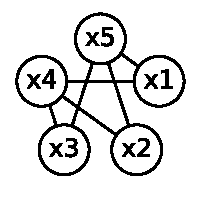
\includegraphics[width=0.21\linewidth]{img/f372738d3845db182fe0b4a3eced9bc2ac778c82a1804f5788cce6bb74ea1beb.pdf}
	\vspace{-1em}
	\captionof{figure}{Contoh Graf}
	\label{fig:algorithm-example}
\end{minipage}

Untuk memperjelas pembahasan sebelumnya, diilustrasikan ulang eksposisi melalui contoh. Dapat diperhatikan graf pada \autoref{fig:algorithm-example}. Graf ini memiliki representasi dalam matriks ketetanggaan sebagai berikut.
\[
	M = \left[ \begin{array}{ccccc}
		0 & 0 & 0 & 1 & 1 \\
		0 & 0 & 0 & 1 & 1 \\
		0 & 0 & 0 & 1 & 1 \\
		1 & 1 & 1 & 0 & 0 \\
		1 & 1 & 1 & 0 & 0
	\end{array} \right]
\]
Menggunakan \foreign{Floyd-Warshall}, didapatkan matriks jarak simpul ke simpul berikut.
\[
	D^{(V)} = \left[ \begin{array}{ccccc}
		0 & 2 & 2 & 1 & 1 \\
		2 & 0 & 2 & 1 & 1 \\
		2 & 2 & 0 & 1 & 1 \\
		1 & 1 & 1 & 0 & 2 \\
		1 & 1 & 1 & 2 & 0
	\end{array} \right]
\]
Selanjutnya, dari membandingkan setiap pasang kolom di matriks jarak, dihasilkan \foreign{distance similarity matrix} berikut.
\[
	B^{(V)} = \left[ \begin{array}{c@{\enspace}c@{\enspace}c@{\enspace}c@{\enspace}c@{\enspace}c@{\enspace}c@{\enspace}c@{\enspace}c@{\enspace}c@{\enspace}}
		\False & \False & \False & \False &  \True & \False & \False & \False & \False &  \True \\
		\False &  \True & \False & \False & \False & \False & \False & \False & \False &  \True \\
		 \True & \False & \False & \False & \False & \False & \False & \False & \False &  \True \\
		 \True &  \True & \False & \False &  \True & \False & \False & \False & \False & \False \\
		 \True &  \True & \False & \False &  \True & \False & \False & \False & \False & \False
	\end{array} \right]
\]
Kolom pertama pada \(B^{(V)}\) dihasilkan dari perbandingan kolom pertama dan kedua pada \(D^{(V)}\), yaitu \((B^{(V)}_{*1}=B^{(V)}_{*2})\), kolom kedua \(B^{(V)}\) dihasilkan dari perbandingan kolom pertama dan ketiga \(D^{(V)}\), yaitu \((B^{(V)}_{*1}=B^{(V)}_{*3})\), kolom ketiga \(B^{(V)}\) dihasilkan dari perbandingan kolom pertama dan keempat \(D^{(V)}\), yaitu \((B^{(V)}_{*1}=B^{(V)}_{*4})\), dan seterusnya, hingga kolom terakhir \(B^{(V)}\) dihasilkan dari perbandingan kolom keempat dan kelima \(D^{(V)}\), yaitu \((B^{(V)}_{*4}=B^{(V)}_{*5})\), sehingga \(B^{(V)}\) memiliki 10 kolom karena terdapat 10 kombinasi pasangan kolom yang dibandingkan dari \(D^{(V)}\). Kemudian, setelah penghapusan, didapat \foreign{reduced distance similarity} berikut.
\[
	P^{(V)} = \left[ \begin{array}{ccccc}
		\False & \False &  \True &  \True \\
		\False &  \True & \False &  \True \\
		 \True & \False & \False &  \True \\
		 \True &  \True &  \True & \False \\
		 \True &  \True &  \True & \False \\
	\end{array} \right]
\] \\
Dapat dilihat seluruh kolom pada \(B^{(V)}\) berisi semua \(\False\) terhapus karena korespondensinya dengan himpunan kosong yang merupakan himpunan bagian dari kolom lainnya. Contohnya, kolom ketiga adalah himpunan bagian dari kolom pertama, sehingga \((B^{(V)}_{*3} | B^{(V)}_{*1}) = B^{(V)}_{*1}\). Dengan demikian, \(P^{(V)}\) terdiri dari sisa kolom-kolom yang tidak saling memuat satu sama lain.

Misal dipilih kolom kedua dari \(P^{(V)}\), yaitu \(P^{(V)}_{*2} = (\False, \True, \False, \True, \True)\). Mengambil semua simpul yang berkoresponden dengan \(\True\), didapat \(W = V[P^{(V)}_{*2}] = \{v_2, v_4, v_5\}\). Lihat bahwa
\[
	(P^{(V)}|W) = \left[ \begin{array}{ccccc}
		\False &  \True & \False &  \True \\
		 \True &  \True &  \True & \False \\
		 \True &  \True &  \True & \False \\
	\end{array} \right]
\]
di mana kolom kedua berisi semua \(\True\). Disimpulkan \(W\) dan semua subset dari \(W\), yaitu \(\{v_2, v_4, v_5\}\), \(\{v_4, v_5\}\), \(\{v_2, v_5\}\), \(\{v_2, v_4\}\), \(\{v_2\}\), \(\{v_4\}\), \(\{v_5\}\), dan \(\emptyset\) bukanlah \foreign{resolving set}.

Contoh \foreign{resolving set} berkardinalitas 3 untuk graf ini adalah \(\{v_1, v_2, v_4\}\). Kemudian, karena ia tidak memiliki \foreign{resolving set} berkardinalitas 2, maka kardinalitas minimum \foreign{resolving set}-nya adalah 3. Sehingga, disimpulkan dimensi metriknya adalah 3.

\subsection{\foreign{Brute-force}}
\label{subsec:bf}

Cara paling sederhana untuk menunjukkan bahwa \(k\) adalah kandidat dimensi matrik yang \foreign{valid} adalah dengan mencoba satu per satu himpunan \(W \subseteq V\) berkardinalitas \(k\) hingga ditemukan \(W\) yang merupakan \foreign{resolving set}. Sebaliknya, untuk menunjukkan bahwa tidak ada \foreign{resolving set} berkardinalitas \(k\), maka harus dicoba habis seluruh kemungkinan himpunan \(W \subseteq V\) berkardinalitas \(k\). Kemudian, untuk menguji apakah \(W\) adalah \foreign{resolving set}, cukup ditunjukkan untuk seluruh kolom di \(P\) bahwa tidak ada \(W\) merupakan himpunan bagian tak sejati dari \(V[P_{*j}]\). Secara terbalik, jika ada saja satu kolom di \(P\) yang menyebabkan \(W \subseteq V[P_{*j}]\), maka \(W\) bukanlah \foreign{resolving set}.

Karena \(P\) berbentuk matriks boolean, akan lebih mudah untuk bekerja dengan representasi \(W\) dalam bentuk boolean juga. Hal ini dapat dilakukan dengan mengkonstruksi vektor boolean \(X \in \Bbb^{|V|}\) yang memiliki sebanyak \(k\) nilai \(\True\). Oleh karena itu, jelas \(W = V[X]\) adalah himpunan berkardinalitas \(k\). Selanjutnya, pengujian apakah \(W\) merupakan himpunan bagian tak sejati dari \(V[P_{*j}]\) dapat dicapai melalui operasi \((X|P_{*j})\). Secara eksplisit:
\[
	\begin{array}{rl}
		(X|P_{*j}) = P_{*j}  &\iff V[X] \subseteq V[P_{*j}] \\
		(X|P_{*j}) \neq P_{*j}  &\iff V[X] \not\subseteq V[P_{*j}]
	\end{array}
\]

Amatilah, untuk menyatakan bahwa tidak ada \foreign{resolving set} berkardinalitas \(k\), harus diuji habis sebanyak \(\binom{|V|}{k}\) kasus. Sedangkan, secara umum, untuk menemukan satu contoh \foreign{resolving set} berkardinalitas \(k\), akan dibutuhkan banyaknya kasus yang perlu diuji kurang dari \(\binom{|V|}{k}\). Maka dari itu, menemukan satu contoh \foreign{resolving set} berkardinalitas \(k\) "lebih murah" dibandingkan menunjukkan tidak ada \foreign{resolving set} berkardinalitas \(k\). Sehingga, desain algoritma yang melakukan pencarian dari bawah, yaitu secara iteratif menaikkan nilai \(k\) hingga menemukan \foreign{resolving set} pertama dan mengambil kardinalitasnya sebagai dimensi metrik, akan "lebih lambat" dibandingkan desain algoritma yang melakukan pencarian dari atas, yaitu secara iteratif menurunkan nilai \(k\) hingga menemukan kardinalitas pertama yang tidak ada \foreign{resolving set}-nya dan mengambil \(k + 1\) sebagai dimensi metrik.

Dengan demikian, diperolehlah formulasi algoritma penentuan dimensi metrik dan dimensi metrik sisi menggunakan pendekatan \foreign{brute-force} sebagaimana tertera pada \autoref{alg:brute-force}.

\begin{example}
	Ambil graf \autoref{fig:algorithm-example}, dan cari dimensi metriknya menggunakan \autoref{alg:brute-force}.
	\begin{enumerate}
		\item Untuk \(k = 5\), ditemukan \(X = (\True, \True, \True, \True, \True)\) sehingga \(W = \{v_1, v_2,\\ v_3, v_4, v_5\}\) adalah \foreign{resolving set}.
		\item Untuk \(k = 4\), ditemukan \(X = (\True, \True, \True, \True, \False)\) sehingga \(W = \{v_1, v_2,\\ v_3, v_4\}\) adalah \foreign{resolving set}.
		\item Untuk \(k = 3\), ditemukan \(X = (\True, \True, \False, \True, \False)\) sehingga \(W = \{v_1, v_2,\\ v_4\}\) adalah \foreign{resolving set}.
		\item Untuk \(k = 2\), secara habis tidak ada \foreign{resolving set} berkardinalitas 2.
	\end{enumerate}
	Disimpulkan bahwa \(2 + 1 = 3\) adalah dimensi metrik dari graf tersebut.
\end{example}

\subsection{\foreign{Boolean Satisfiability}}
\label{subsec:bs}

Pertama-tama, didefinisikan pemetaan injektif \(\boolmap\) dari \(V\) ke variabel boolean di SMT. Catat bahwa variabel boolean di sini bukanlah elemen di \(\Bbb\), melainkan merupakan variabel abstrak di SMT yang nilainya belum ditentukan. Hanya setelah menjalankan \foreign{solver} barulah dihasilkan \foreign{model} yang elemennya di \(\Bbb\). Dengan demikian, variabel-variabel tersebut digunakan untuk mengkonstruksi \foreign{constraint} sehingga \foreign{model} \(\in \Bbb^{|V|}\) menunjukkan \(W \subseteq V\) yang elemen-elemennya berkoresponden dengan elemen di \(V\) yang \(\boolmap(v_i)\)-nya bernilai \(\True\).

Meskipun secara konsep \(\boolmap(v_i)\) adalah variabel abstrak, secara matematis, tidak dibedakan makna \(\boolmap(v_i)\) antara sebelum dan setelah adanya \foreign{model}. Oleh karena itu, secara praktis, tidak ada salahnya menganggap \(\boolmap(v_i) \in \Bbb\). Cukup dibedakan pemaknaan penggunaan ketika dalam konteks \foreign{constraint}. Menggunakan konvensi ini, \(\boolmap(V) = X\) dapat digunakan langsung untuk \foreign{indexing} pada \(V\), sehingga \(W = V[X] \subseteq V\) terdefinisi dengan baik. Sebelum ada \foreign{model}, \(W\) adalah koresponden dari ruang solusi terhadap \foreign{constraint}, dan setelah ada \foreign{model}, solusi \(W\) adalah himpunan nyata.

\begin{example}
	Bila \(\boolmap(v_i) = x_i\), maka untuk simpul-simpul di \autoref{fig:algorithm-example}, didapatkan \(\boolmap(V) = \{x_1, x_2, x_3, x_4, x_5\} = X\). Kemudian, model \(x_3 = x_4 = x_5 = \True, x_1 = x_2 = \False\), menunjukkan koresponden himpunan \(W = \{x_3, x_4, x_5\} \subseteq V\). Dapat digunakan notasi alternatif \(X = (\False, \False, \True, \True, \True)\) menunjukkan model dan \(W = V[X]\) sebagai koresponden himpunannya.
\end{example}

\vspace{-1em}

\begin{algorithm}[H]
	\foreign{Input}:
	\begin{enumerate}
		\item Representasi graf dalam representasi matriks ketetanggaan \(M\).
		\item Mencari dimensi metrik atau dimensi metrik sisi?
	\end{enumerate}
	Prosedur:
	\begin{enumerate}
		\item Hitung \(D^{(V)}\) dari \(M\) menggunakan \foreign{Floyd-Warshall}.
		\item Hitung \(D^{(E)}\) dari \(D^{(V)}\).
		\item Isi \(D\) dengan \(D^{(V)}\) jika mencari dimensi metrik, atau isi \(D\) dengan \(D^{(E)}\) jika mencari dimensi metrik sisi.
		\item Hitung \(B\) dari \(D\).
		\item Hitung \(P\) dari \(B\).
		\item Digunakan variabel \(n\) sebagai banyaknya kolom di \(P\), yaitu \(n :=\) banyak kolom \(P\).
		\item Mulai variabel \(k\) dari banyaknya simpul, yaitu \(k := |V|\).
		\item Selama \(k \geq 0\):
			\begin{enumerate}
				\item Coba satu per satu untuk semua kemungkinan \(X \in \Bbb^{|V|}\) yang memiliki sebanyak \(k\) nilai \(\True\):
					\begin{enumerate}
						\item Mulai variabel \(j\) dari nilai 1, yaitu \(j := 1\).
						\item Selama \(j \leq n\):
							\begin{enumerate}
								\item Jika \((X|P_{*j}) = P_{*j}\), lompat ke tahap (8a).
								\item Tambah \(j\) sebanyak satu, yaitu \(j := j + 1\).
							\end{enumerate}
						\item Lompat ke tahap (8c).
					\end{enumerate}
				\item Lonpat ke tahap (10).
				\item Kurangi \(k\) sebanyak satu, yaitu \(k := k - 1\).
			\end{enumerate}
		\item Simpulkan bahwa 0 adalah dimensi metrik atau dimensi metrik sisi, dan \texttt{BERHENTI}.
		\item Simpulkan bahwa \(k + 1\) adalah dimensi metrik atau dimensi metrik sisi.
	\end{enumerate}
	\caption{\foreign{Brute-force}}
	\label{alg:brute-force}
\end{algorithm}

Kedua, untuk sembarang \(W \subseteq V\), dapat dikonstruksi \foreign{constraint} sedemikian rupa \foreign{model}-nya berkoresponden satu-satu dengan \(W\). Secara umum, variabel yang tidak memiliki restriksi akan memiliki nilai \(\indeterminate\) pada \foreign{model}-nya. Maksud dari \(\indeterminate\) adalah variabel yang bebas; yaitu, tidak peduli apa pun nilai yang ia miliki, kebenaran dari \foreign{constraint} yang ada tidak terpengaruhi oleh variabel tersebut. Ketika \foreign{solver} menghasilkan sebuah \foreign{model}, seluruh variabelnya yang \(\indeterminate\) akan diberi sembarang nilai. Artinya, untuk variabel boolean, ia akan mendapatkan sembarang nilai \(\True\) atau \(\False\).

\begin{example}
	Misalnya \(X = \{x_1, x_2, x_3\}\). \foreign{Constraint} \(\neg x_1\) hanya memaksa terjadinya \(x_1 = \False\). Sementara \(x_2\) dan \(x_3\) secara umum bernilai \(\indeterminate\). Sehingga, meskipun \foreign{model} yang dihasilkan dari \foreign{solver} akan memberi nilai nyata kepada \(x_2\) dan \(x_3\), nilai tersebut diperoleh secara sembarang dari \(\True\) atau \(\False\).
\end{example}

Maka dari itu, agar koresponden \foreign{model}-nya satu-satu dengan himpunan yang dituju, tidak boleh ada variabel yang tidak terestriksi secara tidak sengaja dalam \foreign{constraint} yang dikonstruksikan. Untuk kasus di sini yang memilih tepat \(W\), \foreign{constraint} yang menyatakan pemilihan ini adalah sebagai berikut:

\[
	\combine{\left(}
			{\bigwedge \limits_{\displaystyle v \in W} \boolmap(v)}
	{\right)}{\wedge}{\left(}
			{\bigwedge \limits_{\displaystyle v \in \widetilde{W}} \neg \boolmap(v)}
	{\right)}
\]

\begin{example}
	Untuk \(V = \{v_1, v_2, v_3, v_4, v_5\}\) dan \(W = \{v_3, v_4, v_5\}\), \foreign{constraint} yang menyebabkan koresponden satu-satu antara \(W\) dan \(V[X]\) adalah: \(\neg x_1 \wedge \neg x_2 \wedge x_3 \wedge x_4 \wedge x_5\).
\end{example}

Ketiga, untuk sembarang \(W \subseteq V\), dapat dikonstruksi \foreign{constraint} sedemikian rupa \foreign{model}-nya berkoresponden satu-satu dengan \(\Pcal(W)\). Dapat diperhatikan pada konstruksi \foreign{constraint} sebelumnya betapa pentingnya konteks \(V\) yang dimaksud relatif terhadap \(W\) karena \foreign{model} yang menyatakan \(W\) tidak hanya didefinisikan oleh \(W\) sendiri, tetapi juga oleh \(\widetilde{W} = V \setminus W\). Dalam konstruksi \foreign{constraint} untuk \(\Pcal(W)\) ini, hubungan tersebut menjadi lebih kritikal. Karena, terbalik dari perspektif \foreign{power set} pada umumnya, dalam bentuk \foreign{constraint}, definisi \foreign{power set} justru dilihat dari elemen-elemennya yang tidak ada di \(W\). Lebih formalnya dinyatakan oleh ekspresi berikut:
\[
	\bigwedge \limits_{\displaystyle v \in \widetilde{W}} \neg \boolmap(v)
\]
Dengan kata lain, seluruh kemungkinan \foreign{model} yang memenuhi \foreign{constraint} ini bebas menetapkan keanggotaan elemen-elemen di \(W\), dan hanya yang di \(W\), sehingga menyatakan seluruh kombinasi yang merepresentasikan \(\Pcal(W)\). Dengan demikian, ruang solusi dari \foreign{model} yang memenuhi \foreign{constraint} tersebut ekivalen dengan \(\Pcal(W)\).

\begin{example}
	Untuk \(V = \{v_1, v_2, v_3, v_4, v_5\}\) dan \(W = \{v_3, v_4, v_5\}\), \foreign{constraint} yang menyebabkan koresponden satu-satu antara \(\Pcal(W)\) dan \(V[X]\) adalah: \(\neg x_1 \wedge \neg x_2\). Setiap \foreign{model} yang memenuhi \(\neg x_1 \wedge \neg x_2\) mewakili satu subset dari \(\{v_3, v_4, v_5\}\).
\end{example}

Akhirnya, dapat dibahas konstruksi \foreign{constraint boolean satisfiability} yang menunjukkan \foreign{resolving set}. Ingat kembali, untuk setiap kolom di \(P\), himpunan \(V[P_{*j}]\) serta seluruh himpunan bagiannya bukanlah \foreign{resolving set}. Maka, \(W \subseteq V\) adalah \foreign{resolving set} jika dan hanya jika \(W\) tidak ada di \(\Pcal(V[P_{*j}])\) untuk setiap kolom di \(P\). Secara formal, ini dapat dinyatakan sebagai berikut:

\[
	\bigwedge \limits_{\displaystyle P_{*j} \in P} \neg \left( \bigwedge \limits_{\displaystyle v \in \widetilde{V[P_{*j}]}} \neg \boolmap(v) \right)
\]
Sedemikian rupa dapat disederhakan menjadi:
\begin{equation}
	\bigwedge \limits_{\displaystyle P_{*j} \in P} \enspace \bigvee \limits_{\displaystyle v \in V[\sim\!P_{*j}]} \boolmap(v)
	\label{eq:boolean-satisfiability-natural}
\end{equation}

\begin{example}
	Ambil graf \autoref{fig:algorithm-example}. \foreign{Constraint} yang berkorespondensi dengan \foreign{resolving set}-nya adalah:
		\[
			( x_1 \vee x_2 ) \wedge \ ( x_1 \vee x_3 ) \wedge \ ( x_2 \vee x_3 ) \wedge \ ( x_4 \vee x_5 )
		\]
	\label{ex:boolean-satisfiability-natural}
\end{example}

Secara teori, \foreign{constraint} \autoref{eq:boolean-satisfiability-natural} sudah berbentuk \foreign{conjunctive normal form} (CNF). Akan tetapi, ketika menunjukkan \(\unsat\) menggunakan SMT, efektivitasnya sangat bergantung pada \foreign{conflict driven learning}, yaitu metode "penalaran" yang digunakan oleh \foreign{solver} untuk melakukan pemangkasan ruang pencarian. Salah satu sifat yang digunakan oleh \foreign{conflict driven learning} adalah bentuk CNF yang terdiri dari suku-suku positif maupun suku-suku negatif. Sedangkan \autoref{eq:boolean-satisfiability-natural} sepenuhnya hanya memuat suku-suku positif. Bentuk yang sudah diperoleh ini dapat ditransformasikan agar juga memuat suku-suku negatif dengan memfaktorkan keluar "pemilihan" himpunan kosong, dengan cara berikut:

\begin{equation}
	\begin{array}{l}
		\displaystyle \bigwedge \limits_{\displaystyle P_{*j} \in P} \enspace \combine{\left(}{\False}{\right)}{\vee}{\left(}{\bigvee \limits_{\displaystyle v \in V[\sim\!P_{*j}]} \boolmap(v)}{\right)} \\ [18pt]
		\displaystyle = \bigwedge \limits_{\displaystyle P_{*j} \in P} \enspace \combine{\left(}{\combine{\left(}{\bigvee \limits_{\displaystyle v \in V[P_{*j}]} \boolmap(v)}{\right)}{\wedge}{\left(}{\neg \bigvee \limits_{\displaystyle v \in V[P_{*j}]} \boolmap(v)}{\right)}}{\right)}{\vee}{\left(}{\bigvee \limits_{\displaystyle v \in V[\sim\!P_{*j}]} \boolmap(v)}{\right)} \\ [18pt]
		\displaystyle = \bigwedge \limits_{\displaystyle P_{*j} \in P} \enspace \combine{\left(}{\combine{\left(}{\bigvee \limits_{\displaystyle v \in V[P_{*j}]} \boolmap(v)}{\right)}{\vee}{\left(}{\bigvee \limits_{\displaystyle v \in V[\sim\!P_{*j}]} \boolmap(v)}{\right)}}{\right)}{\\[18pt]\qquad\qquad\wedge}{\left(}{\combine{\left(}{\neg \bigvee \limits_{\displaystyle v \in V[P_{*j}]} \boolmap(v)}{\right)}{\vee}{\left(}{\bigvee \limits_{\displaystyle v \in V[\sim\!P_{*j}]} \boolmap(v)}{\right)}}{\right)} \\ [18pt]
		\displaystyle = \bigwedge \limits_{\displaystyle P_{*j} \in P} \enspace \combine{\left(}{\bigvee \limits_{\displaystyle v \in V} \boolmap(v)}{\right)}{\wedge}{\left(}{\bigvee \limits_{\displaystyle v \in V[P_{*j}]} \boolmap(v)\ \implies \bigvee \limits_{\displaystyle v \in V[\sim\!P_{*j}]} \boolmap(v)}{\right)} \\ [18pt]
		\displaystyle = \combine{\left(}{\bigvee \limits_{\displaystyle v \in V} \boolmap(v)}{\right)}{\wedge}{\left(}{\bigwedge \limits_{\displaystyle P_{*j} \in P} \enspace \left( \bigvee \limits_{\displaystyle v \in V[P_{*j}]} \boolmap(v)\ \implies \bigvee \limits_{\displaystyle v \in V[\sim\!P_{*j}]} \boolmap(v) \right)}{\right)} \\ [18pt]
	\end{array}
	\label{eq:boolean-satisfiability}
\end{equation}

\begin{example}
	Berikut adalah hasil dari pemfaktoran \autoref{ex:boolean-satisfiability-natural}.
	\[
		\begin{array}{c}
			x_1 \vee x_2 \vee x_3 \vee x_4 \vee x_5 \\ [4pt]
			x_3 \vee x_4 \vee x_5 \implies x_1 \vee x_2 \\
			x_2 \vee x_4 \vee x_5 \implies x_1 \vee x_3 \\
			x_1 \vee x_4 \vee x_5 \implies x_2 \vee x_3 \\
			x_1 \vee x_2 \vee x_3 \implies x_4 \vee x_5
		\end{array}
	\]
	\label{ex:boolean-satisfiability}
\end{example}

Karena ruang solusi \foreign{model} yang memenuhi \foreign{constraint} tersebut sudah menunjukkan \foreign{resolving set}, maka algoritma yang perlu dirancang cukup mencari \foreign{resolving set} dengan kardinalitas terendah dari ruang solusi. Ini dapat dilakukan dengan mudah menggunakan \foreign{constraint} \(\AtLeast\) dan \(\AtMost\) yang memaksa banyaknya variabel boolean bernilai \(\True\) secara berturut-turut kurang dari atau sama dengan dan lebih dari atau sama dengan \(k\).

Secara historis, SMT paling efektif ketika bekerja langsung dengan bentuk CNF. Akan tetapi, SMT \foreign{modern} sudah tidak lagi terbatasi oleh \foreign{implementation detail} seperti ini, sebagaimana yang telah dibahasa pada Pendahuluan. Maka dari itu, \foreign{solver} sekarang sudah memiliki \foreign{higher level construct} dan justru lebih banyak diuntungkan ketika bekerja langsung dalam bentuk tersebut. \foreign{Constraint} \(\AtLeast\) dan \(\AtMost\) merupakan salah satu contoh dari \foreign{higher level construct} yang ada dalam SMT. Namun, tidak ada salahnya untuk memahami bagaimana bentuk-bentuk ini dapat direpresentasikan menggunakan operasi konjungsi dan disjungsi yang lebih sederhana. Berikut adalah salah satu \foreign{encoding} yang mungkin dilakukan untuk menyatakan kedua \foreign{constraint} tersebut. Catat, notasi \(\displaystyle \binom{V}{n} = \{W \subseteq V : |V| = n\}\) menunjukkan himpunan yang memuat seluruh himpunan bagian \(V\) dengan kardinalitas \(n\).
\[
	\AtLeast(V, n) = \displaystyle \bigvee \limits_{\displaystyle W \in \binom{V}{n}} \enspace \bigwedge \limits_{\displaystyle v \in W} \boolmap(v)
\]

\[
	\AtMost(V, n) = \displaystyle \bigvee \limits_{\displaystyle W \in \binom{V}{n}} \enspace \bigwedge \limits_{\displaystyle v \in \widetilde{W}} \neg \boolmap(v)
\]

Secara umum, menunjukkan \(\sat\) dalam SMT lebih murah dari pada menunjukkan \(\unsat\). Hal ini karena secara fundamental, SMT adalah proses mencari \foreign{model}. Oleh karena itu, untuk menunjukkan \(\sat\), cukup dicari satu saja contoh yang memenuhi \foreign{constraint}. Sedangkan untuk menunjukkan \(\unsat\), harus secara habis dibuktikan bahwa tidak ada satu pun \foreign{model} yang dapat memenuhi \foreign{constraint}.

Dengan demikian, didapatkan desain \autoref{alg:boolean-satisfiability} yang melakukan pencarian dari atas. Digunakan \(\AtLeast\) dan \(\AtMost\) secara bersamaan untuk memaksa mencari \foreign{model} berkardinalitas tepat sama dengan \(k\). Dimulai dari nilai \(k\) tertinggi, lalu secara iteratif menurunkan nilai \(k\) hingga menemukan kardinalitas pertama yang menyebabkan \(\unsat\), dan mengambil \(k + 1\) sebagai dimensi metrik.

\begin{example}
	Ambil graf \autoref{fig:algorithm-example}, dan cari dimensi metriknya menggunakan \autoref{alg:boolean-satisfiability}. \foreign{Constraint} yang digunakan sesuai dengan \autoref{ex:boolean-satisfiability}. Kemudian, untuk masing-masing tahap berikut, diterapkan \foreign{constraint} tambahan \(\AtLeast\) dan \(\AtMost\) sama dengan \(k\).
	\begin{enumerate}
		\item Untuk \(k = 5\), ditemukan \(\sat\).
		\item Untuk \(k = 4\), ditemukan \(\sat\).
		\item Untuk \(k = 3\), ditemukan \(\sat\).
		\item Untuk \(k = 2\), ditemukan \(\unsat\).
	\end{enumerate}
	Disimpulkan bahwa \(2 + 1 = 3\) adalah dimensi metrik dari graf tersebut.
\end{example}

\vspace{-0.5em}

\begin{algorithm}[H]
	\foreign{Input}:
	\begin{enumerate}
		\item Representasi graf dalam representasi matriks ketetanggaan \(M\).
		\item Mencari dimensi metrik atau dimensi metrik sisi?
	\end{enumerate}
	Prosedur:
	\begin{enumerate}
		\item[1--5.] Sama seperti pada \autoref{alg:brute-force}.
		\setcounter{enumi}{5}
		\item Tambahkan \foreign{constraint} berdasarkan \autoref{eq:boolean-satisfiability} dari \(P\) ke \foreign{solver} SMT.
		\item Mulai variabel \(k\) dari banyaknya simpul, yaitu \(k := |V|\).
		\item Selama \(k \geq 0\):
			\begin{enumerate}
					\item Tambahkan \foreign{constraint} \(\AtLeast\) dan \(\AtMost\) sama dengan \(k\).
					\item Jalankan \foreign{solver} untuk mencari \foreign{model}.
					\item Jika dihasilkan \(\unsat\), lompat ke tahap (10).
					\item Hapus \foreign{constraint} \(\AtLeast\) dan \(\AtMost\) yang ditambahkan sebelumnya.
					\item Kurangi \(k\) sebanyak satu, yaitu \(k := k - 1\).
			\end{enumerate}
		\item Simpulkan bahwa 0 adalah dimensi metrik atau dimensi metrik sisi, dan \texttt{BERHENTI}.
		\item Simpulkan bahwa \(k + 1\) adalah dimensi metrik atau dimensi metrik sisi.
	\end{enumerate}
	\caption{\foreign{Boolean Satisfiability}}
	\label{alg:boolean-satisfiability}
\end{algorithm}

\subsection{\foreign{Linear Integer Arithmetic}}

Seperti pemetaan injektif \(\boolmap\), di sini didefinisikan pemetaan injektif \(\intmap\) dari \(V\) ke variabel \foreign{integer} di SMT. Dengan membatasi \(0 \leq \intmap(v_i) \leq 1\), seperti halnya koresponden keanggotaan simpul dalam \(W\) bergantung dari nilai \(\True\) untuk \(\boolmap(v_i)\), nilai \(1\) untuk \(\intmap(v_i)\) menunjukkan korespondensi keanggotaan dan nilai \(0\) untuk tidak. Sehingga, pemetaan \foreign{resolving set} ke dalam \foreign{constraint boolean satisfiability} dapat diangkat secara langsung ke bentuk \foreign{linear integer arithmetic} dengan melakukan translasi berikut:
\[
	\bigvee \limits_{\displaystyle v \in W} \boolmap(v)
	\iff
	\sum \limits_{\displaystyle v \in W} \intmap(v) \enspace \geq 1
\]
Didapat bentuk dari \autoref{eq:boolean-satisfiability-natural} dalam \foreign{linear integer arithmetic} sebagai berikut:
\begin{equation}
	\bigwedge \limits_{\displaystyle P_{*j} \in P} \enspace \sum \limits_{\displaystyle v \in V[\sim\!P_{*j}]} \intmap(v) \enspace \geq 1
	\label{eq:linear-integer-arithmetic-natural}
\end{equation}

\begin{example}
	Ambil graf \autoref{fig:algorithm-example}. Misalnya \(\intmap(v_i) = x_i\), maka \foreign{constraint} yang berkorespondensi dengan \foreign{resolving set}-nya dalam \foreign{linear integer arithmetic} adalah:
	\[
		\begin{array}{c}
			x_1 + x_2 \geq 1 \\
			x_1 + x_3 \geq 1 \\
			x_2 + x_3 \geq 1 \\
			x_4 + x_5 \geq 1 \\ [4pt]
			0 \leq x_1 \leq 1,\enspace
			0 \leq x_2 \leq 1,\enspace
			0 \leq x_3 \leq 1,\enspace
			0 \leq x_4 \leq 1,\enspace
			0 \leq x_5 \leq 1
		\end{array}
	\]
\end{example}

Selanjutnya, untuk \foreign{constraint} \(\AtLeast\) dan \(\AtMost\), dapat dinyatakan dalam \foreign{linear integer arithmetic} dengan lebih sederhana sebagai:
\begin{equation}
	\sum \limits_{\displaystyle v \in V} \intmap(v) \enspace = k
	\label{eq:linear-integer-arithmetic-cardinality}
\end{equation}

Perhatikan bentuk jumlahan ini yang lebih ekspresif dari pada \(\AtLeast\) dan \(\AtMost\). Menggunakan persamaan ini, \autoref{eq:linear-integer-arithmetic-natural} dapat ditransformasi menjadi relatif terhadap kardinalitas \(k\) seperti berikut:
\begin{equation}
	\bigwedge \limits_{\displaystyle P_{*j} \in P} \enspace \sum \limits_{\displaystyle v \in V[P_{*j}]} \intmap(v) \enspace \leq k - 1
	\label{eq:linear-integer-arithmetic}
\end{equation}

Sama seperti transformasi \autoref{eq:boolean-satisfiability-natural} ke \autoref{eq:boolean-satisfiability} yang membantu \foreign{conflict driven learning}, transformasi di \foreign{linear integer arithmetic} dari \autoref{eq:linear-integer-arithmetic-natural} ke \autoref{eq:linear-integer-arithmetic} juga membantu SMT dalam pemangkasan ruang pencarian.

\begin{example}
	Untuk graf \autoref{fig:algorithm-example}, \foreign{constraint} yang berkorespondensi dengan \foreign{resolving set} berkardinalitas \(k\) adalah:
	\[
		\begin{array}{c}
			x_1 + x_2 + x_3 + x_4 + x_5 = k \\ [4pt]
			x_3 + x_4 + x_5 \leq k - 1 \\
			x_2 + x_4 + x_5 \leq k - 1 \\
			x_1 + x_4 + x_5 \leq k - 1 \\
			x_1 + x_2 + x_3 \leq k - 1 \\ [4pt]
			0 \leq x_1 \leq 1,\enspace
			0 \leq x_2 \leq 1,\enspace
			0 \leq x_3 \leq 1,\enspace
			0 \leq x_4 \leq 1,\enspace
			0 \leq x_5 \leq 1
		\end{array}
	\]
	\label{ex:linear-integer-arithmetic-constraint}
\end{example}

\noindent Dengan demikian, didapatkan desain algoritma yang menggunakan \foreign{linear integer arithmetic}.

\begin{example}
	Ambil graf \autoref{fig:algorithm-example}, dan cari dimensi metriknya menggunakan \autoref{alg:linear-integer-arithmetic}. Setelah menetapkan \foreign{constraint} \(0 \leq x_i \leq 1\) untuk setiap variabel \foreign{integer}-nya, \foreign{constraint} yang digunakan pada setiap tahapannya bersesuaian dengan yang telah tertera pada \autoref{ex:linear-integer-arithmetic-constraint}.
	\begin{enumerate}
		\item Untuk \(k = 5\), ditemukan \(\sat\).
		\item Untuk \(k = 4\), ditemukan \(\sat\).
		\item Untuk \(k = 3\), ditemukan \(\sat\).
		\item Untuk \(k = 2\), ditemukan \(\unsat\).
	\end{enumerate}
	Disimpulkan bahwa \(2 + 1 = 3\) adalah dimensi metrik dari graf tersebut.
\end{example}

\begin{algorithm}[H]
	\foreign{Input}:
	\begin{enumerate}
		\item Representasi graf dalam representasi matriks ketetanggaan \(M\).
		\item Mencari dimensi metrik atau dimensi metrik sisi?
	\end{enumerate}
	Prosedur:
	\begin{enumerate}
		\item[1--5.] Sama seperti pada \autoref{alg:boolean-satisfiability}.
		\setcounter{enumi}{5}
		\item Tambahkan \foreign{constraint} \(0 \leq \intmap(v_i) \leq 1\) untuk semua \(v_i \in V\) ke \foreign{solver} SMT.
		\item Mulai variabel \(k\) dari banyaknya simpul, yaitu \(k := |V|\).
		\item Selama \(k \geq 0\):
			\begin{enumerate}
					\item Tambahkan \foreign{constraint} berdasarkan \autoref{eq:linear-integer-arithmetic-cardinality}, dan berdasarkan \autoref{eq:linear-integer-arithmetic} dari \(P\), ke \foreign{solver} SMT.
					\item Jalankan \foreign{solver} untuk mencari \foreign{model}.
					\item Jika dihasilkan \(\unsat\), lompat ke tahap (10).
					\item Hapus \foreign{constraint} yang ditambahkan dari tahap (8a) sebelumnya.
					\item Kurangi \(k\) sebanyak satu, yaitu \(k := k - 1\).
			\end{enumerate}
		\item Simpulkan bahwa 0 adalah dimensi metrik atau dimensi metrik sisi, dan \texttt{BERHENTI}.
		\item Simpulkan bahwa \(k + 1\) adalah dimensi metrik atau dimensi metrik sisi.
	\end{enumerate}
	\caption{\foreign{Linear Integer Arithmetic}}
	\label{alg:linear-integer-arithmetic}
\end{algorithm}

\vspace{-0.5em}

\subsection{\foreign{Pseudo Boolean}}

Pada akhirnya, sampailah di penghujung desain algoritma dimensi metrik menggunakan SMT. Dapat dicermati bentuk \foreign{constraint} yang terdapat dalam \foreign{linear integer arithmetic} sudah sesuai dengan representasi \foreign{constraint} yang dibutuhkan dalam \foreign{pseudo boolean}. Maka dari itu, konstruksi \foreign{constraint} dapat diturunkan kembali menggunakan variabel boolean dari pada \foreign{integer}, tetapi menggunakan teori yang lebih tinggi dari \foreign{boolean satisfiability}, yaitu \foreign{pseudo boolean}. Di sini, didapatkan kembali representasi natural keanggotaan sebagai nilai \(\True\), dan secara bersamaan dapat diekspresikan bentuk \foreign{constraint} yang memuat logika kardinalitas secara lebih natural. Dengan demikian, \autoref{eq:linear-integer-arithmetic-cardinality} dan \autoref{eq:linear-integer-arithmetic} dapat translasikan langsung menjadi pseudo boolean sebagai berikut:

\begin{equation}
	\sum \limits_{\displaystyle v \in V} \boolmap(v) \enspace = k
	\label{eq:pseudo-boolean-cardinality}
\end{equation}

\begin{equation}
	\bigwedge \limits_{\displaystyle P_{*j} \in P} \enspace \sum \limits_{\displaystyle v \in V[P_{*j}]} \boolmap(v) \enspace \leq k - 1
	\label{eq:pseudo-boolean}
\end{equation}

Meskipun perubahan yang dilakukan hanyalah membawa turun dari \foreign{linear integer arithmetic} ke \foreign{pseudo boolean}, dengan bentuk \foreign{constraint} yang kurang lebih sama persis, ketika tidak ada \foreign{expresiveness} yang hilang, maka secara umum \foreign{solver} yang menggunakan \foreign{pseudo boolean} akan lebih efektif dibandingkan yang menggunakan \foreign{linear integer arithmetic}.

\begin{example}
	Ambil graf \autoref{fig:algorithm-example}. Jika \(\boolmap(v_i) = x_i\), maka \foreign{constraint} yang berkorespondensi dengan \foreign{resolving set} berkardinalitas \(k\) adalah:
	\[
		\begin{array}{c}
			x_1 + x_2 + x_3 + x_4 + x_5 = k \\ [4pt]
			x_3 + x_4 + x_5 \leq k - 1 \\
			x_2 + x_4 + x_5 \leq k - 1 \\
			x_1 + x_4 + x_5 \leq k - 1 \\
			x_1 + x_2 + x_3 \leq k - 1
		\end{array}
	\]
	\label{ex:pseudo-boolean-constraint}
\end{example}

\noindent Sehingga, didapat desain algoritma yang menggunakan \foreign{pseudo boolean}.

\begin{example}
	Untuk graf \autoref{fig:algorithm-example}, mencari dimensi metriknya menggunakan \autoref{alg:pseudo-boolean}, dapat dilakukan dengan mengambil pada setiap tahapannya \foreign{constraint} yang telah tertera pada \autoref{ex:pseudo-boolean-constraint}.
	\begin{enumerate}
		\item Untuk \(k = 5\), ditemukan \(\sat\).
		\item Untuk \(k = 4\), ditemukan \(\sat\).
		\item Untuk \(k = 3\), ditemukan \(\sat\).
		\item Untuk \(k = 2\), ditemukan \(\unsat\).
	\end{enumerate}
	Disimpulkan bahwa \(2 + 1 = 3\) adalah dimensi metrik dari graf tersebut.
\end{example}

\vspace{-1em}

\begin{algorithm}[H]
	\foreign{Input}:
	\begin{enumerate}
		\item Representasi graf dalam representasi matriks ketetanggaan \(M\).
		\item Mencari dimensi metrik atau dimensi metrik sisi?
	\end{enumerate}
	Prosedur:
	\begin{enumerate}
		\item[1--5.] Sama seperti pada \autoref{alg:linear-integer-arithmetic}.
		\setcounter{enumi}{5}
		\item Mulai variabel \(k\) dari banyaknya simpul, yaitu \(k := |V|\).
		\item Selama \(k \geq 0\):
			\begin{enumerate}
					\item Tambahkan \foreign{constraint} berdasarkan \autoref{eq:pseudo-boolean-cardinality}, dan berdasarkan \autoref{eq:pseudo-boolean} dari \(P\), ke \foreign{solver} SMT.
					\item Jalankan \foreign{solver} untuk mencari \foreign{model}.
					\item Jika dihasilkan \(\unsat\), lompat ke tahap (9).
					\item Hapus \foreign{constraint} yang ditambahkan dari tahap (7a) sebelumnya.
					\item Kurangi \(k\) sebanyak satu, yaitu \(k := k - 1\).
			\end{enumerate}
		\item Simpulkan bahwa 0 adalah dimensi metrik atau dimensi metrik sisi, dan \texttt{BERHENTI}.
		\item Simpulkan bahwa \(k + 1\) adalah dimensi metrik atau dimensi metrik sisi.
	\end{enumerate}
	\caption{\foreign{Pseudo Boolean}}
	\label{alg:pseudo-boolean}
\end{algorithm}

\vspace{-1em}


\section{Evaluasi Algoritma}
\label{sec:implementation}

Seluruh algoritma yang telah dideskripsikan pada \autoref{sec:alg} diimplementasikan dalam bahasa pemrograman \foreign{Python} versi 3.14 serta menggunakan \foreign{libraries} yang tersedia melalui \foreign{pip} dan \foreign{conda-forge}. Di antaranya adalah \foreign{NetworkX}, yang menyediakan fungsi untuk \foreign{decoding} dan \foreign{encoding} format \verb`graph6`; \foreign{NumPy}, yang menyediakan fungsi untuk melakukan operasi matriks secara efisien; \foreign{SciPy}, yang menyediakan implementasi algoritma \foreign{Floyd-Warshall}; dan \foreign{Z3-solver}, yang menyediakan \foreign{binding} untuk menggunakan \foreign{solver} Z3 melalui \foreign{Python}. Informasi lebih lanjut mengenai cara mengakses kode implementasi ini dapat ditemukan pada \cref{app:code}.

Melanjutkan pembahasan pada \autoref{sec:data}, total graf kecil yang akan dicari dimensi metrik dan dimensi metrik sisinya adalah sebanyak 273192 graf. Untuk graf besar, dipilih dari graf bersimpul 10 hingga graf bersimpul 50 dengan interval 5 simpul, dan diambil masing-masing sebanyak 50 graf. Sehingga, total graf besar yang akan dicari dimensi metrik dan dimensi metrik sisinya adalah sebanyak 450 graf. Dengan demikian, total graf yang akan dievaluasi adalah sebanyak 273642 graf. Rincian lebih detailnya dapat dilihat pada \autoref{tab:graph-count}.

Terdapat 4 macam algoritma yang masing-masing digunakan untuk mencari dimensi metrik dan dimensi metrik sisi pada sebanyak 273642 graf. Dapat dicatat bahwa setiap komputasi bersifat saling independen, atau disebut juga sebagai \foreign{embarrassingly parallel}. Oleh karena itu, secara keseluruhan, komputasi ini dapat dipercepat dengan menggunakan \foreign{CPU} yang memiliki \foreign{multi-core}, selama semua \foreign{core} yang digunakan identik satu sama lain. Untuk tugas akhir ini, digunakan \foreign{CPU Intel i7-1185G7} dengan \foreign{4 physical cores} yang masing-masing memiliki kapabilitas \foreign{hyperthreading}, sehingga ada sebanyak \foreign{8 logical cores} yang dapat digunakan.

\vspace{-0.3em}

\begin{center}
	\renewcommand{\minipagewidth}{0.35\linewidth}
	\begin{minipage}[\minipagealign]{\minipagewidth}
	\centering
	\captionof{table}{\centering Data Graf}
	\vspace{-0.5em}
	\resizetofit{
		\begin{tabular}{|c|c|}
			\hline
			Graf Bersimpul & Banyak Graf \\ \hline
			2             & 1           \\ \hline
			3             & 2           \\ \hline
			4             & 6           \\ \hline
			5             & 21          \\ \hline
			6             & 112         \\ \hline
			7             & 853         \\ \hline
			8             & 11117       \\ \hline
			9             & 261080      \\ \hline
			10            & 50          \\ \hline
			15            & 50          \\ \hline
			20            & 50          \\ \hline
			25            & 50          \\ \hline
			30            & 50          \\ \hline
			35            & 50          \\ \hline
			40            & 50          \\ \hline
			45            & 50          \\ \hline
			50            & 50          \\ \hline
		\end{tabular}
	\label{tab:graph-count}
	}
\end{minipage}

\end{center}

\vspace{-0.1em}

Meskipun antar komputasi bersifat \foreign{embarrassingly parallel}, implementasi setiap komputasinya sendiri secara internal tidak bersifat parallel. Maka dari itu, diperlakukan batas waktu eksekusi pada setiap algoritma. Batasan waktu ini diimplementasikan bukan pada total waktu eksekusi masing-masing algoritma, melainkan pada waktu eksekusi di setiap iterasi kardinalitasnya. Adapun tahap yang dibatasi adalah tahap \((8a)\) pada \autoref{alg:brute-force} dan \autoref{alg:boolean-satisfiability}, tahap \((8b)\) pada \autoref{alg:linear-integer-arithmetic}, dan tahap \((7b)\) pada \autoref{alg:pseudo-boolean}. Batas waktu yang dipilih untuk tugas akhir ini adalah selama 5 menit. Ditekankan kembali batas waktu ini adalah pada setiap iterasi kardinalitas, sehingga jelas total waktu eksekusi dapat lebih dari 5 menit.

Akhirnya, hasil dari setiap komputasi pada individu graf adalah total waktu eksekusi dan, bila algoritma tidak diberhentikan karena melebihi batas waktu, dimensi metrik atau dimensi metrik sisinya. Pembahasan pada \autoref{sec:discussion-small} dan \autoref{sec:discussion-large} langsung mencakup statistik dari hasil semua eksekusi yang telah diperoleh. Sedangkan hasil eksekusi spesifik secara per individual tidak dibahas. Informasi mengenai cara mengakses hasil eksekusi yang masih berbentuk komputasi individual dapat ditemukan pada \cref{app:result}.


\section{Pembahasan Hasil Eksekusi Graf Kecil}
\label{sec:discussion-small}

Pertama, dibahas hasil eksekusi untuk graf kecil. Untuk seluruh algoritma dan untuk dimensi metrik maupun dimensi metrik sisi, tidak ada hasil evaluasi yang gagal karena melewati batas waktu. Sehingga, untuk seluruh 273192 graf kecil, berhasil diidentifikasi dimensi metrik dan dimensi metrik sisinya. Rincian frekuensi graf berdasarkan dimensi metrik dapat dilihat dalam \autoref{tab:freq-md-small}, dan rincian frekuensi graf berdasarkan dimensi metrik sisi dapat dilihat dalam \autoref{tab:freq-emd-small}. Kedua tabel ini berlaku untuk seluruh \autoref{alg:brute-force}, \autoref{alg:boolean-satisfiability}, \autoref{alg:linear-integer-arithmetic}, dan \autoref{alg:pseudo-boolean}, menunjukkan secara \foreign{experimental} bahwa semua implementasi algoritma benar, sekaligus secara tidak langsung menunjukkan bahwa teori formulasi setiap algoritma benar untuk menentukan dimensi metrik dan dimensi metrik sisi, karena semuanya menghasilkan frekuensi yang sama.

Dari data ini, dapat diilustrasikan perbedaan antara invarian graf dimensi metrik dan invarian graf dimensi metrik sisi. Dapat diperhatikan \autoref{fig:hist-md-8}, yaitu histogram frekuensi graf berdasarkan dimensi metrik, dan \autoref{fig:hist-emd-8}, yaitu histogram frekuensi graf berdasarkan dimensi metrik sisi. Meskipun kedua histogram menggunakan graf bersimpul 8, gambaran ini dapat memberikan intuisi mengenai sebaran dimensi metrik dan sebaran dimensi metrik sisi pada graf dengan banyak simpul lebih besar. Dapat diamati bahwa untuk graf dengan \(n\) simpul, sebaran dimensi metrik cenderung berat di kiri \(\dfrac{n}{2}\) sedangkan sebaran dimensi metrik sisi cenderung berat di kanan \(\dfrac{n}{2}\).

Dari data frekuensi ini juga terlihat bahwa eksistensi dimensi metrik dan dimensi metrik sisi minimum mirip, karena hanya ada satu graf yang memiliki dimensi metrik minimum dan hanya ada satu graf pula yang memiliki dimensi metrik sisi minimum. Namun, eksistensi dimensi metrik dan dimensi metrik sisi maksimum berbeda, karena hanya ada satu graf yang berdimensi metrik maksimum, tetapi ada banyak graf yang berdimensi metrik sisi maksimum.

Selanjutnya, untuk membandingkan waktu eksekusi antar algoritma, dihitung rata-rata waktu eksekusi untuk setiap graf dengan \(n\) simpul. Akan tetapi, sebagaimana telah dibahas dalam \autoref{subsec:bf} mengenai pengujian habis dan dalam \autoref{subsec:bs} mengenai menunjukkan \(\unsat\), tidaklah masuk akal untuk menghitung rata-rata waktu eksekusi langsung dari semua graf dengan banyak simpul yang sama. Hal ini karena waktu eksekusi sangat dipengaruhi oleh nilai invarian dimensi metrik maupun dimensi metrik sisi yang dimiliki oleh setiap graf. Oleh karena itu, untuk setiap graf bersimpul \(n\), dipilih graf berdasarkan frekuensi dimensi metrik terbanyak dan dimensi metrik sisi terbanyak.

Untuk graf bersimpul 2 hingga 9, frekuensi dimensi metrik terbanyak berturut-turut adalah 1, 1, 2, 2, 2, 2, 3, 3, 3, dan frekuensi dimensi metrik sisi terbanyak berturut-turut adalah 0, 1, 2, 3, 4, 4, 5, 5.  Rata-rata waktu eksekusi dihitung berdasarkan banyaknya simpul \(n\) dan frekuensi dimensi metrik atau dimensi metrik sisi terbanyak. Hasil perhitungan rata-rata waktu eksekusi setiap algoritma untuk menentukan dimensi metrik pada graf kecil dapat dilihat pada \autoref{tab:mean-md-small}, dan rata-rata waktu eksekusi setiap algoritma menentukan dimensi metrik sisi pada graf kecil dapat dilihat pada \autoref{tab:mean-emd-small}.

Akhirnya, rata-rata waktu eksekusi yang telah diperoleh untuk membandingkan waktu eksekusi setiap algoritma dapat diilustrasikan lebih jelas sebagai grafik tren. Untuk dimensi metrik, tren ini dapat diamati pada \autoref{fig:trend-md-small}, dan untuk dimensi metrik sisi, tren ini dapat diamati pada \autoref{fig:trend-emd-small}. Terlihat bahwa, untuk graf kecil, waktu eksekusi \autoref{alg:brute-force} selalu paling cepat, sedangkan waktu eksekusi \autoref{alg:linear-integer-arithmetic} selalu paling lambat.

\begin{landscape}
\begin{center}
	\renewcommand{\minipagewidth}{0.475\linewidth}

	\vphantom{}
	\vfill

	\begin{minipage}[\minipagealign]{\minipagewidth}
	\centering
	\captionof{table}{\centering Frekuensi Dimensi Metrik Graf Kecil}
	\resizetofit{
		\begin{tabular}{|c|rrrrrrrr|}
			\hline \multirow{2}{*}{\begin{tabular}[c]{@{}c@{}}Dimensi\\ Metrik\end{tabular}} & \multicolumn{8}{c|}{Banyak Simpul} \\ \cline{2-9} & \multicolumn{1}{c|}{2} & \multicolumn{1}{c|}{3} & \multicolumn{1}{c|}{4} & \multicolumn{1}{c|}{5} & \multicolumn{1}{c|}{6} & \multicolumn{1}{c|}{7} & \multicolumn{1}{c|}{8} & \multicolumn{1}{c|}{9} \\ \hline 1 & \multicolumn{1}{r|}{1} & \multicolumn{1}{r|}{1} & \multicolumn{1}{r|}{1} & \multicolumn{1}{r|}{1} & \multicolumn{1}{r|}{1} & \multicolumn{1}{r|}{1} & \multicolumn{1}{r|}{1} & 1 \\ \hline 2 & \multicolumn{1}{r|}{} & \multicolumn{1}{r|}{1} & \multicolumn{1}{r|}{4} & \multicolumn{1}{r|}{13} & \multicolumn{1}{r|}{62} & \multicolumn{1}{r|}{275} & \multicolumn{1}{r|}{1710} & 12061 \\ \hline 3 & \multicolumn{1}{r|}{} & \multicolumn{1}{r|}{} & \multicolumn{1}{r|}{1} & \multicolumn{1}{r|}{6} & \multicolumn{1}{r|}{39} & \multicolumn{1}{r|}{488} & \multicolumn{1}{r|}{8116} & 216432 \\ \hline 4 & \multicolumn{1}{r|}{} & \multicolumn{1}{r|}{} & \multicolumn{1}{r|}{} & \multicolumn{1}{r|}{1} & \multicolumn{1}{r|}{9} & \multicolumn{1}{r|}{77} & \multicolumn{1}{r|}{1145} & 29958 \\ \hline 5 & \multicolumn{1}{r|}{} & \multicolumn{1}{r|}{} & \multicolumn{1}{r|}{} & \multicolumn{1}{r|}{} & \multicolumn{1}{r|}{1} & \multicolumn{1}{r|}{11} & \multicolumn{1}{r|}{130} & 2415 \\ \hline 6 & \multicolumn{1}{r|}{} & \multicolumn{1}{r|}{} & \multicolumn{1}{r|}{} & \multicolumn{1}{r|}{} & \multicolumn{1}{r|}{} & \multicolumn{1}{r|}{1} & \multicolumn{1}{r|}{14} & 196 \\ \hline 7 & \multicolumn{1}{r|}{} & \multicolumn{1}{r|}{} & \multicolumn{1}{r|}{} & \multicolumn{1}{r|}{} & \multicolumn{1}{r|}{} & \multicolumn{1}{r|}{} & \multicolumn{1}{r|}{1} & 16 \\ \hline 8 & \multicolumn{1}{r|}{} & \multicolumn{1}{r|}{} & \multicolumn{1}{r|}{} & \multicolumn{1}{r|}{} & \multicolumn{1}{r|}{} & \multicolumn{1}{r|}{} & \multicolumn{1}{r|}{} & 1 \\ \hline
		\end{tabular}
	}
\end{minipage}

	\hspace{2em}
	\begin{minipage}[\minipagealign]{\minipagewidth}
	\centering
	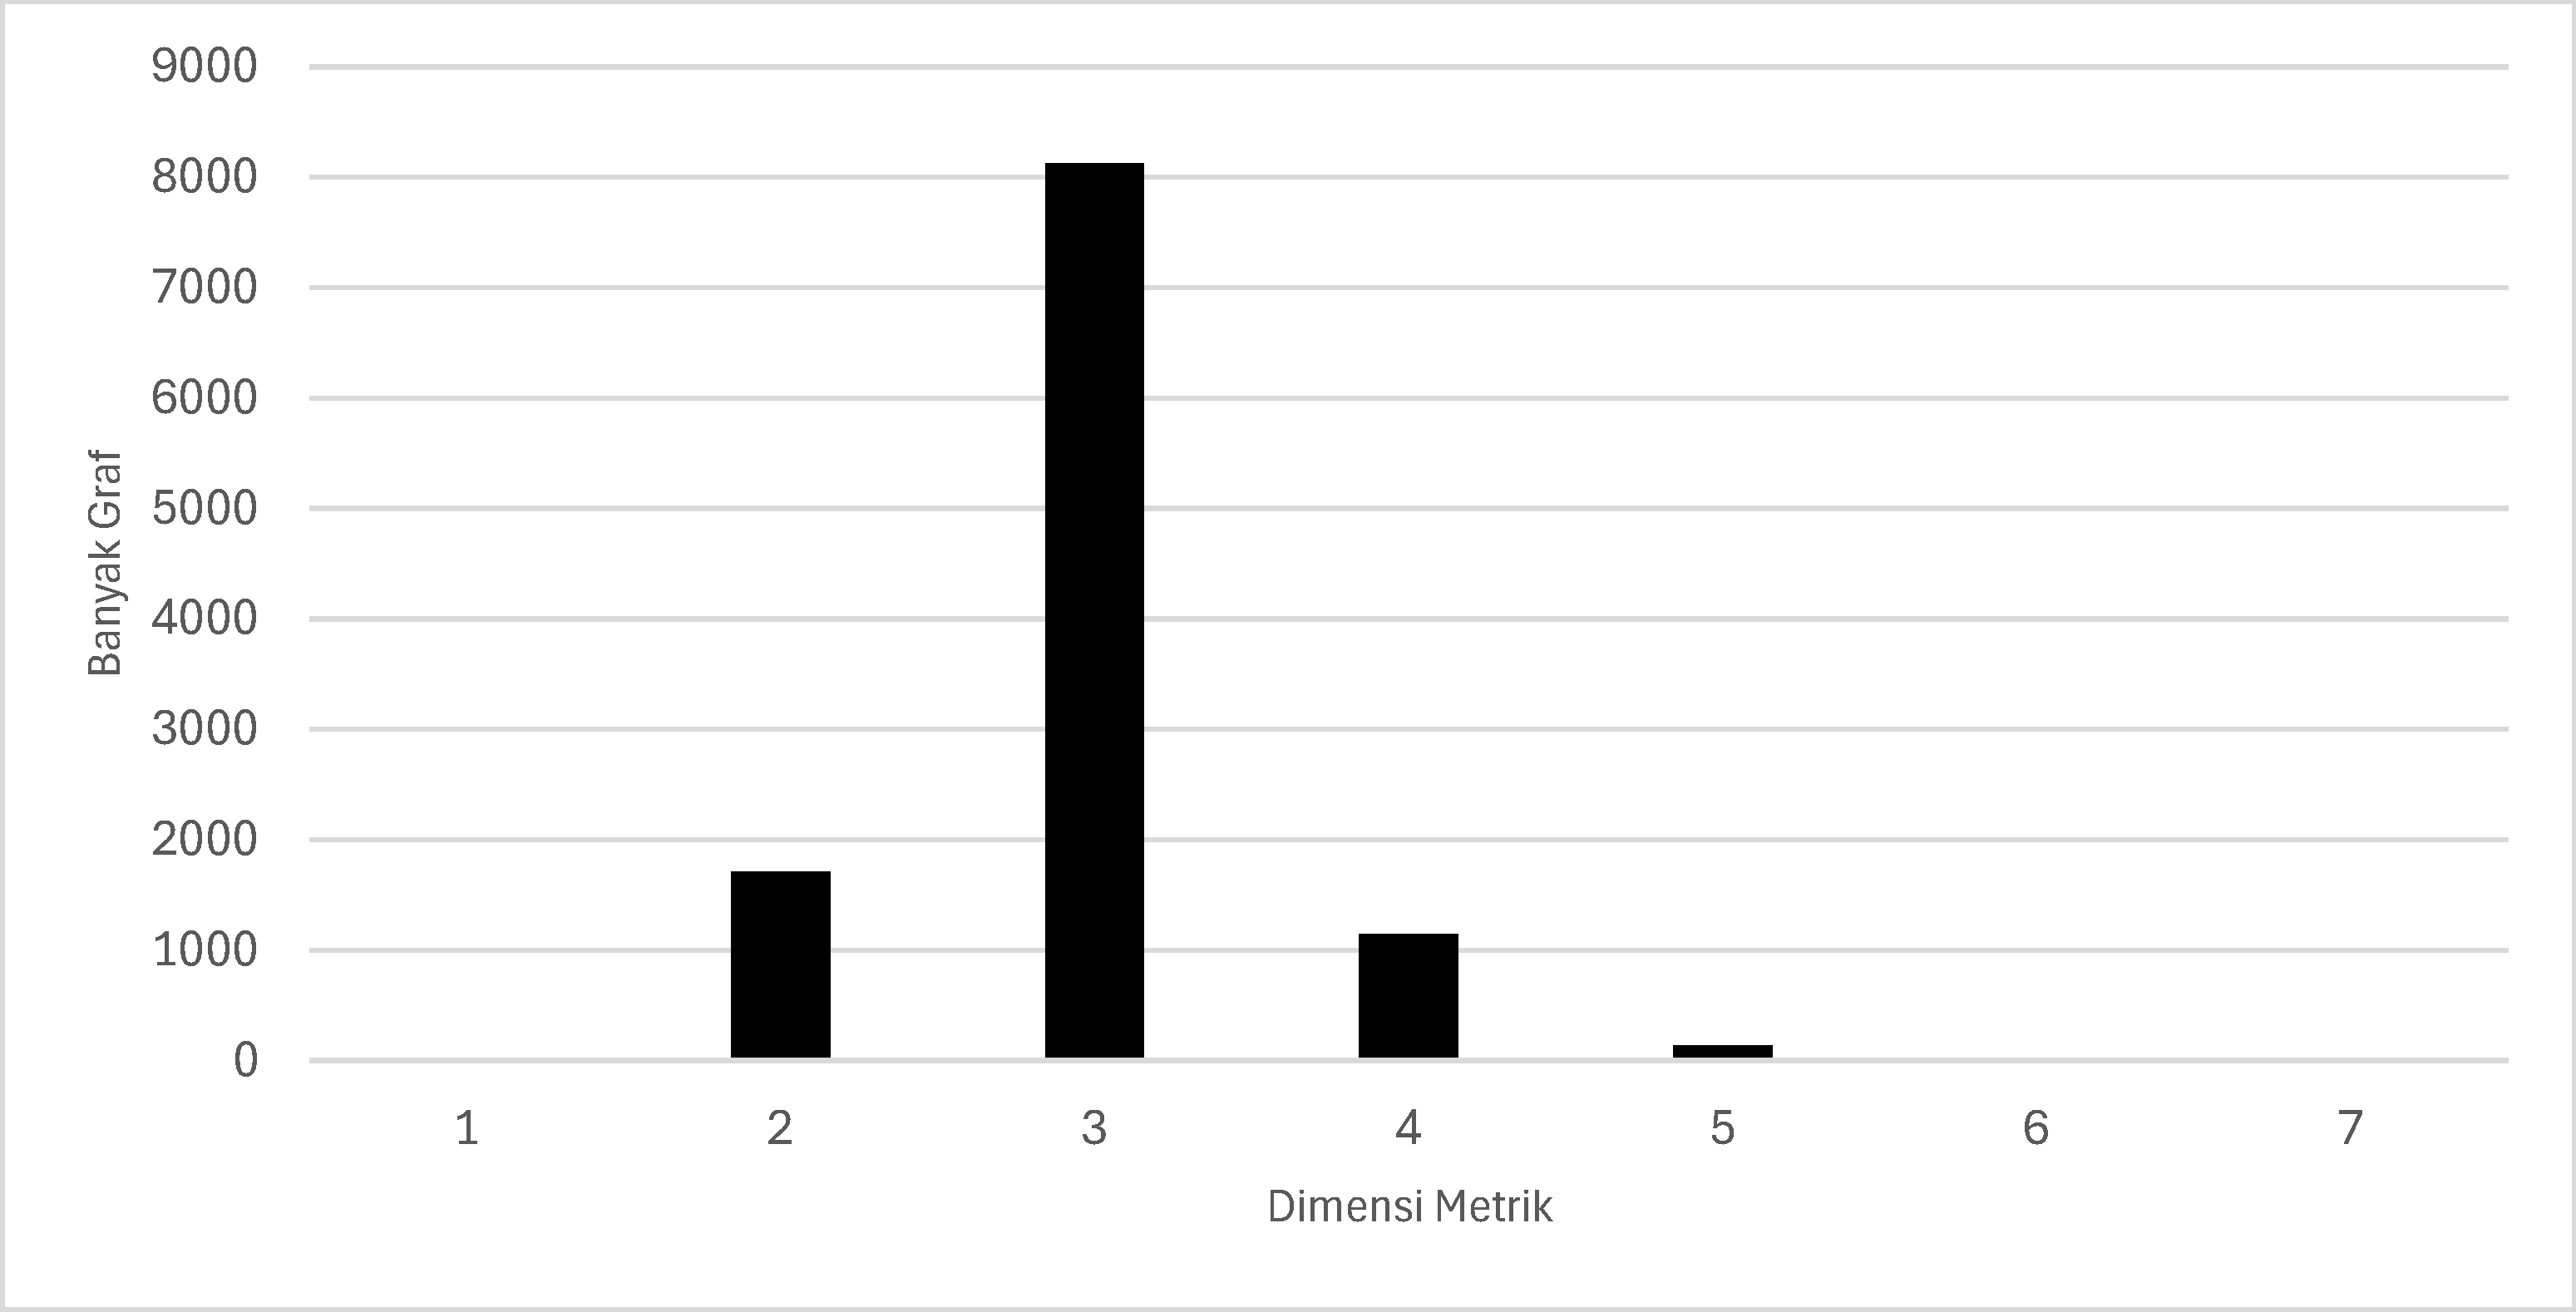
\includegraphics[width=\linewidth]{img/hist-md-8.pdf}
	\captionof{figure}{\centering Histogram Dimensi Metrik Graf Bersimpul 8}
\end{minipage}


	\vspace{2em}

	\begin{minipage}[\minipagealign]{\minipagewidth}
	\centering
	\captionof{table}{\centering Frekuensi Dimensi Sisi Metrik Graf Kecil}
	\resizetofit{
		\begin{tabular}{|c|rrrrrrrr|}
			\hline \multirow{2}{*}{\begin{tabular}[c]{@{}c@{}}Dimensi\\ Metrik Sisi\end{tabular}} & \multicolumn{8}{c|}{Graf Bersimpul} \\ \cline{2-9} & \multicolumn{1}{c|}{2} & \multicolumn{1}{c|}{3} & \multicolumn{1}{c|}{4} & \multicolumn{1}{c|}{5} & \multicolumn{1}{c|}{6} & \multicolumn{1}{c|}{7} & \multicolumn{1}{c|}{8} & \multicolumn{1}{c|}{9} \\ \hline 0 & \multicolumn{1}{r|}{1} & \multicolumn{1}{r|}{} & \multicolumn{1}{r|}{} & \multicolumn{1}{r|}{} & \multicolumn{1}{r|}{} & \multicolumn{1}{r|}{} & \multicolumn{1}{r|}{} & \\ \hline 1 & \multicolumn{1}{r|}{} & \multicolumn{1}{r|}{1} & \multicolumn{1}{r|}{1} & \multicolumn{1}{r|}{1} & \multicolumn{1}{r|}{1} & \multicolumn{1}{r|}{1} & \multicolumn{1}{r|}{1} & 1 \\ \hline 2 & \multicolumn{1}{r|}{} & \multicolumn{1}{r|}{1} & \multicolumn{1}{r|}{3} & \multicolumn{1}{r|}{6} & \multicolumn{1}{r|}{17} & \multicolumn{1}{r|}{40} & \multicolumn{1}{r|}{108} & 292 \\ \hline 3 & \multicolumn{1}{r|}{} & \multicolumn{1}{r|}{} & \multicolumn{1}{r|}{2} & \multicolumn{1}{r|}{9} & \multicolumn{1}{r|}{38} & \multicolumn{1}{r|}{198} & \multicolumn{1}{r|}{1148} & 7414 \\ \hline 4 & \multicolumn{1}{r|}{} & \multicolumn{1}{r|}{} & \multicolumn{1}{r|}{} & \multicolumn{1}{r|}{5} & \multicolumn{1}{r|}{42} & \multicolumn{1}{r|}{330} & \multicolumn{1}{r|}{3566} & 49742 \\ \hline 5 & \multicolumn{1}{r|}{} & \multicolumn{1}{r|}{} & \multicolumn{1}{r|}{} & \multicolumn{1}{r|}{} & \multicolumn{1}{r|}{14} & \multicolumn{1}{r|}{236} & \multicolumn{1}{r|}{4081} & 97009 \\ \hline 6 & \multicolumn{1}{r|}{} & \multicolumn{1}{r|}{} & \multicolumn{1}{r|}{} & \multicolumn{1}{r|}{} & \multicolumn{1}{r|}{} & \multicolumn{1}{r|}{48} & \multicolumn{1}{r|}{1995} & 78723 \\ \hline 7 & \multicolumn{1}{r|}{} & \multicolumn{1}{r|}{} & \multicolumn{1}{r|}{} & \multicolumn{1}{r|}{} & \multicolumn{1}{r|}{} & \multicolumn{1}{r|}{} & \multicolumn{1}{r|}{218} & 26401 \\ \hline 8 & \multicolumn{1}{r|}{} & \multicolumn{1}{r|}{} & \multicolumn{1}{r|}{} & \multicolumn{1}{r|}{} & \multicolumn{1}{r|}{} & \multicolumn{1}{r|}{} & \multicolumn{1}{r|}{} & 1498 \\ \hline
		\end{tabular}
	}
	\label{tab:freq-emd-small}
\end{minipage}

	\hspace{2em}
	\begin{figure}
	\centering
	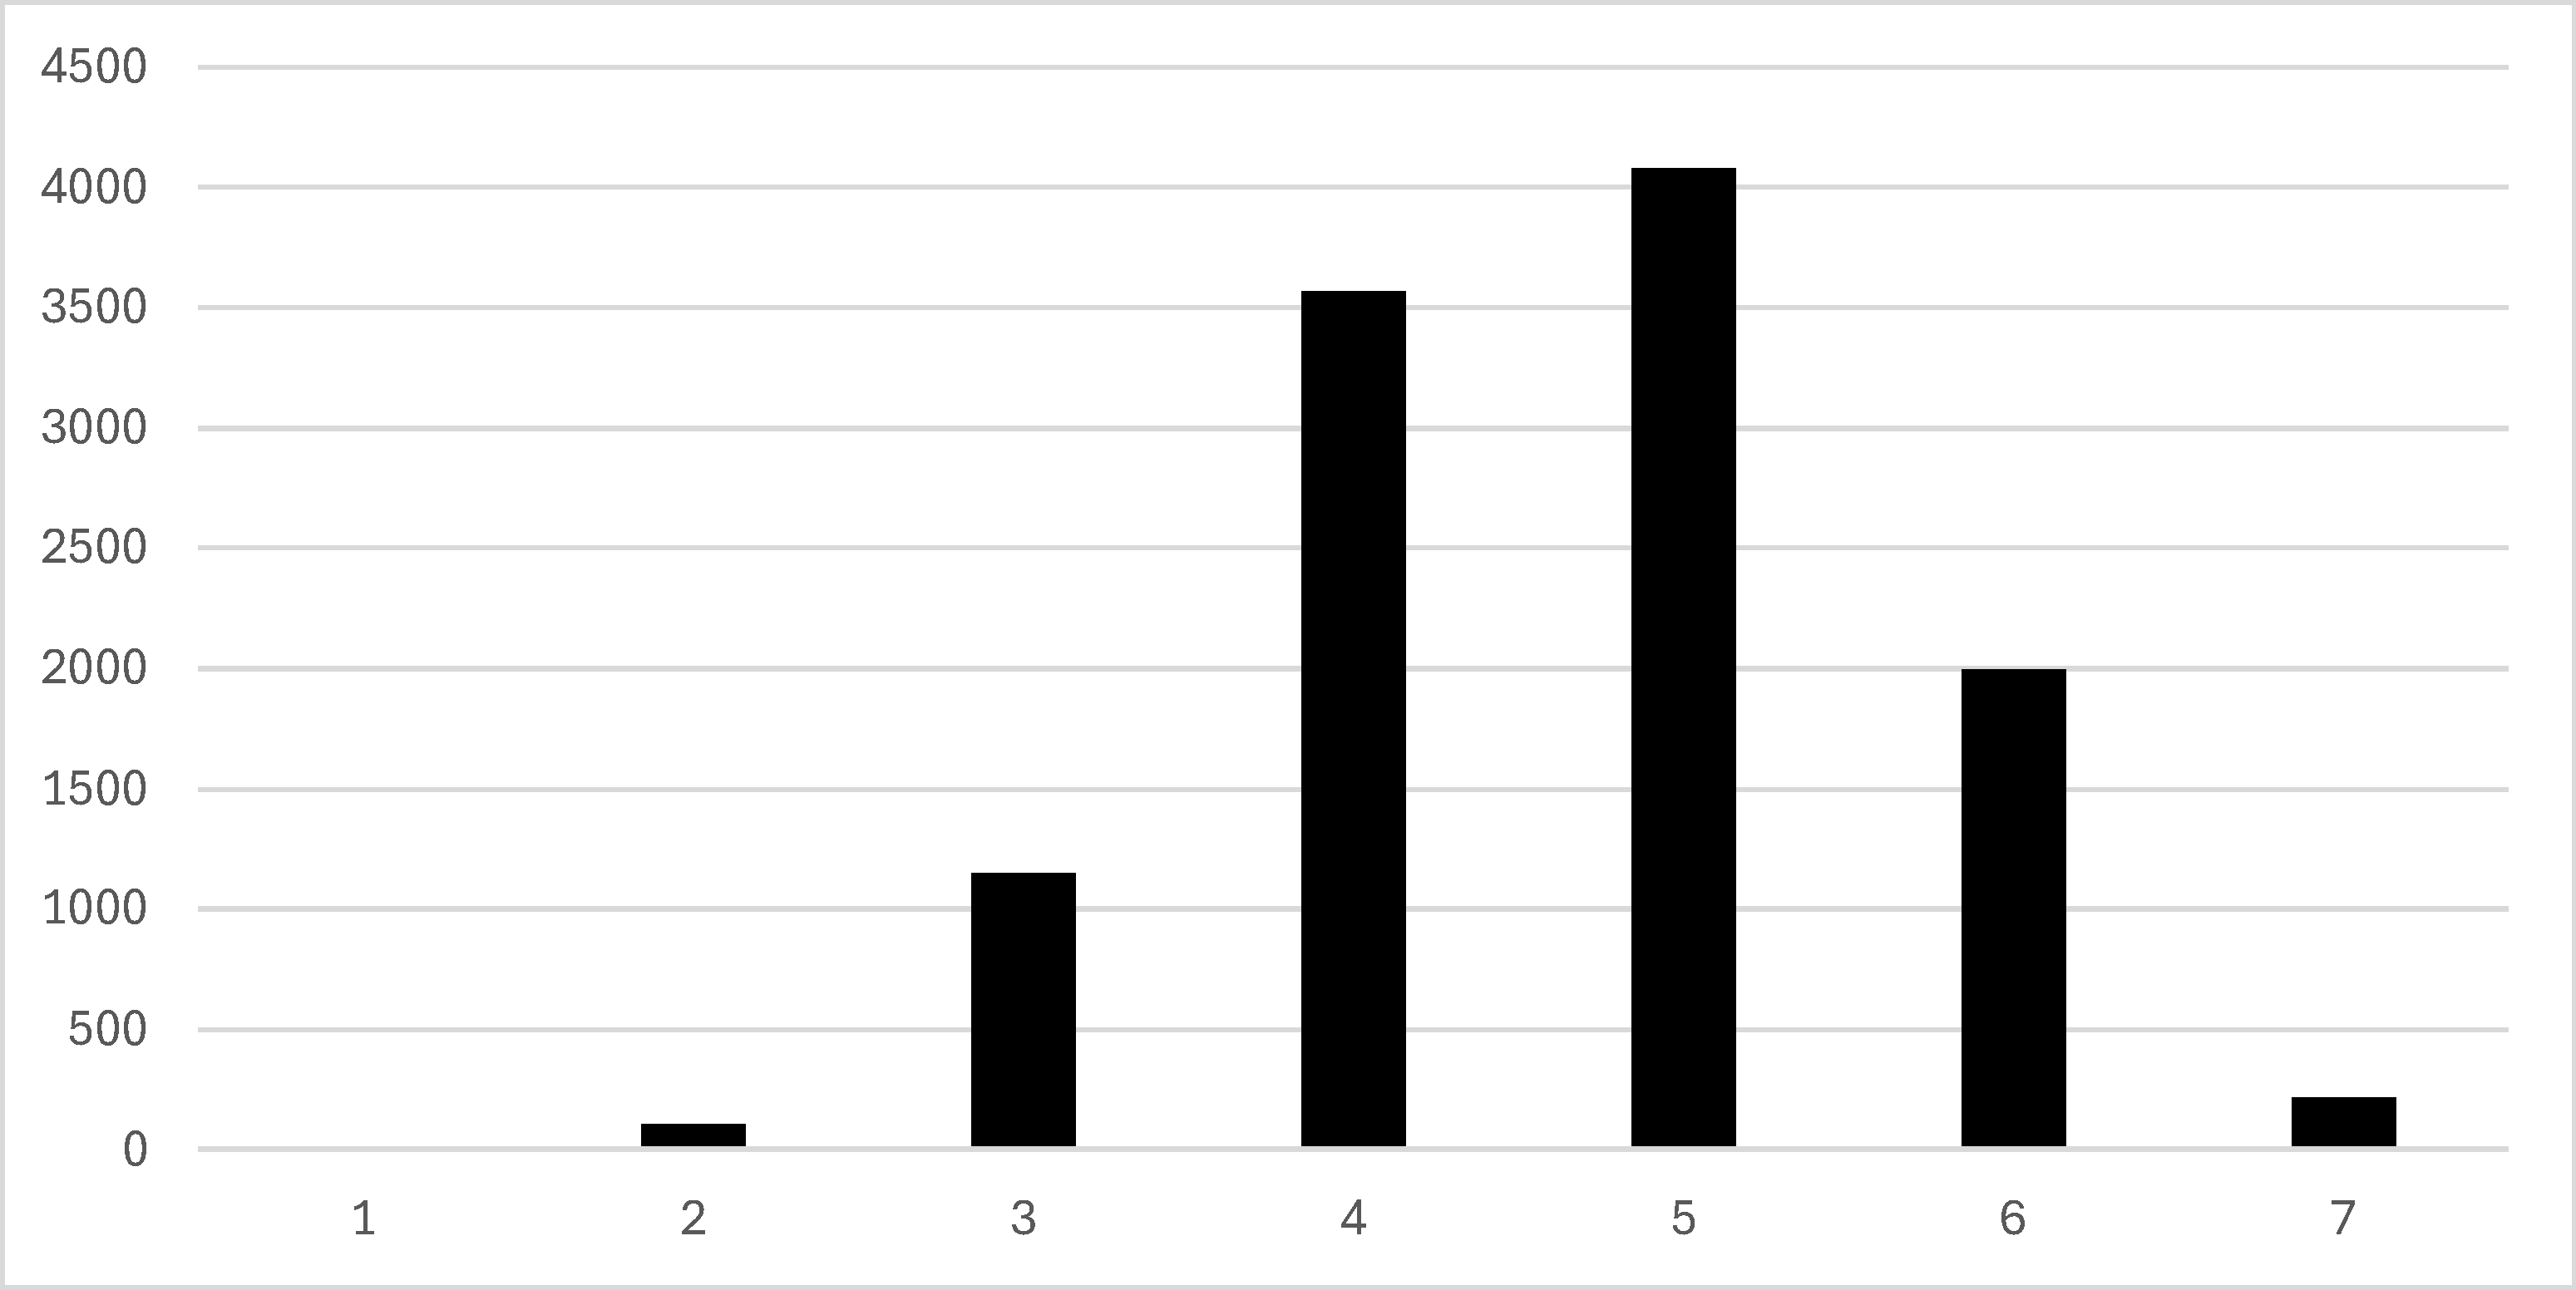
\includegraphics[width=.75\linewidth]{img/hist-emd-8.pdf}
	\caption{Histogram Dimensi Metrik Sisi Graf Bersimpul 8}
\end{figure}


	\vfill \vfill \vfill
\end{center}
\end{landscape}

\begin{landscape}
\begin{center}
	\renewcommand{\minipagewidth}{0.475\linewidth}

	\vphantom{}
	\vfill

	\begin{table}
	\centering
	\caption{Rata-Rata Waktu Eksekusi Dimensi Metrik Graf Kecil (Detik)}
	\begin{tabular}{|c|c|r|r|r|r|}
	\hline
	\begin{tabular}[c]{@{}c@{}}Dimensi\\ Metrik\end{tabular} & \begin{tabular}[c]{@{}c@{}}Banyak\\ Simpul\end{tabular} & \multicolumn{1}{c|}{\foreign{Brute-force}} & \multicolumn{1}{c|}{\begin{tabular}[c]{@{}c@{}}\foreign{Boolean}\\ \foreign{Satisfiability}\end{tabular}} & \multicolumn{1}{c|}{\begin{tabular}[c]{@{}c@{}}\foreign{Linear Integer}\\ \foreign{Arithmetic}\end{tabular}} & \multicolumn{1}{c|}{\begin{tabular}[c]{@{}c@{}}\foreign{Pseudo}\\ \foreign{Boolean}\end{tabular}} \\ \hline
	1                                                        & 2                                                       & .156965                         & .174657                                                                              & .186278                                                                                 & .170794                                                                      \\ \hline
	1                                                        & 3                                                       & .153144                         & .173771                                                                              & .061201                                                                                 & .003076                                                                      \\ \hline
	2                                                        & 4                                                       & .000947                         & .009032                                                                              & .028977                                                                                 & .003894                                                                      \\ \hline
	2                                                        & 5                                                       & .001206                         & .006250                                                                              & .034587                                                                                 & .005617                                                                      \\ \hline
	2                                                        & 6                                                       & .001573                         & .008373                                                                              & .043509                                                                                 & .007274                                                                      \\ \hline
	3                                                        & 7                                                       & .002507                         & .011181                                                                              & .052244                                                                                 & .010301                                                                      \\ \hline
	3                                                        & 8                                                       & .002948                         & .014158                                                                              & .068935                                                                                 & .014817                                                                      \\ \hline
	3                                                        & 9                                                       & .003770                         & .018461                                                                              & .093387                                                                                 & .021154                                                                      \\ \hline
	\end{tabular}
\end{table}

	\hspace{2em}
	\begin{figure}
	\centering
	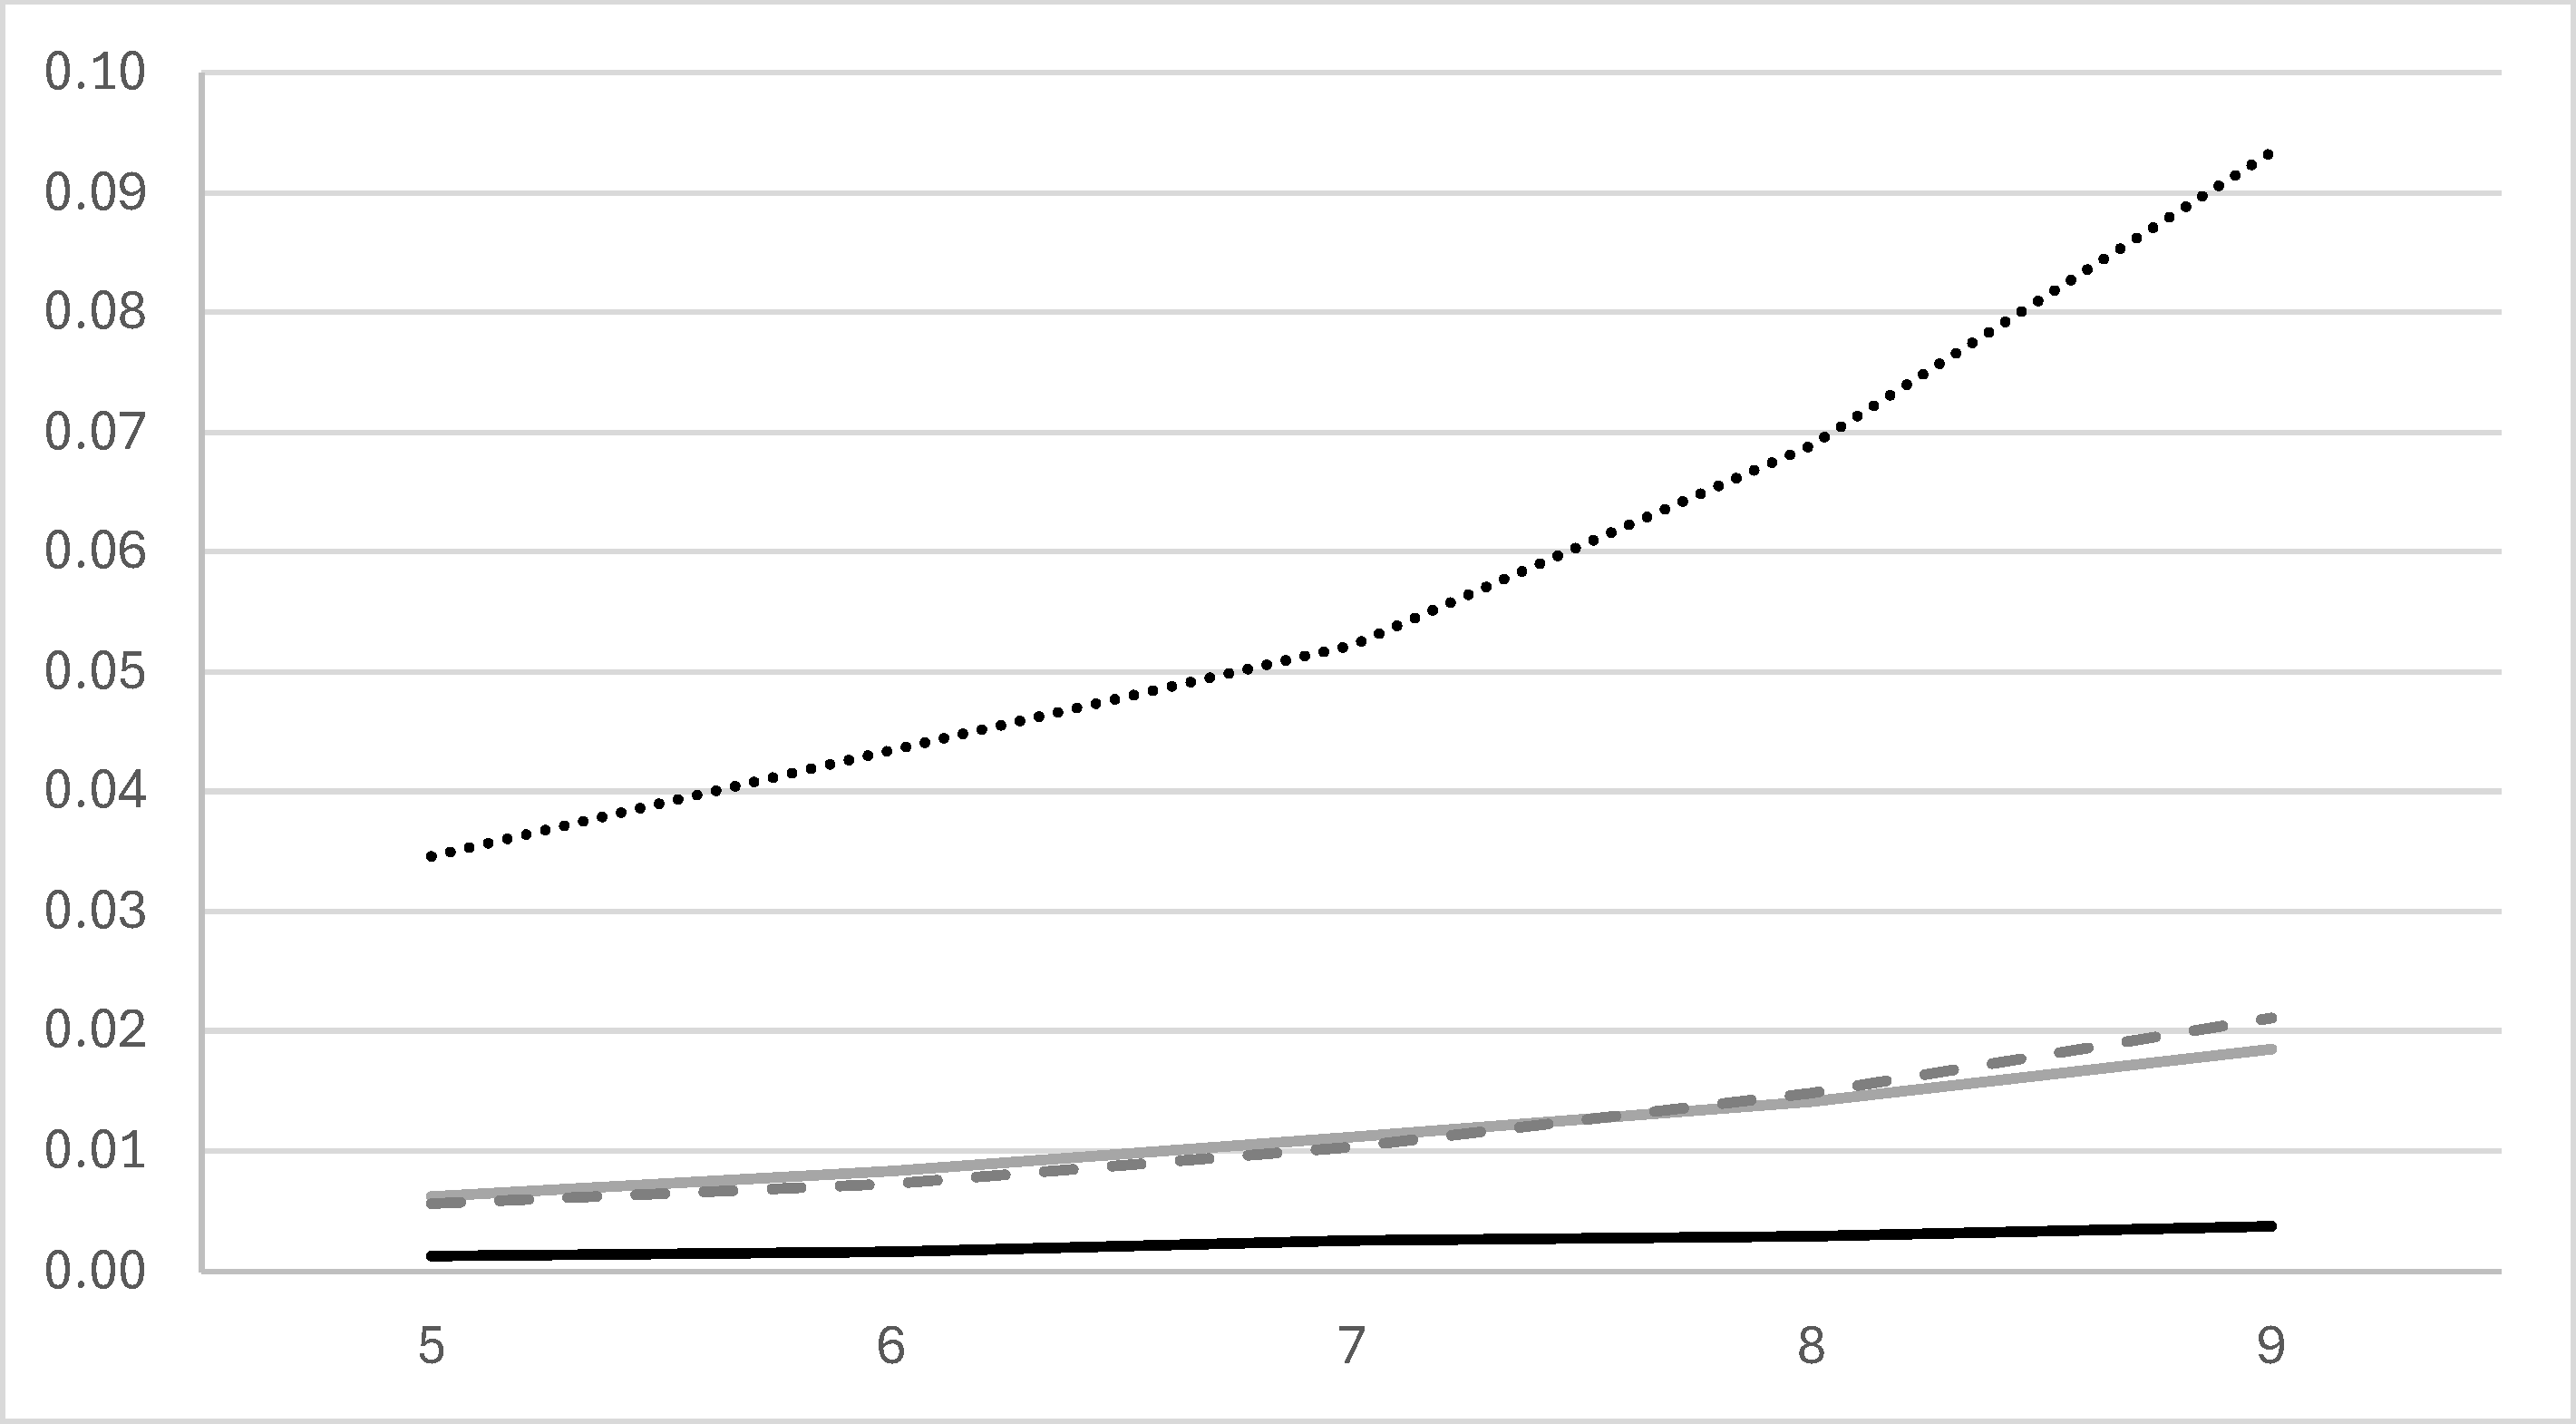
\includegraphics[width=.75\linewidth]{img/trend-md-small.pdf}
	\caption{Trend Dimensi Metrik Graf Kecil}
\end{figure}


	\vspace{2em}

	\begin{minipage}[\minipagealign]{\minipagewidth}
	\centering
	\captionof{table}{\centering Rata-Rata Waktu Eksekusi\\ Dimensi Metrik Sisi Graf Kecil}
	\resizetofit{
		\begin{tabular}{|c|c|r|r|r|r|}
			\hline \begin{tabular}[c]{@{}c@{}}Dimensi\\ Metrik Sisi\end{tabular} & \begin{tabular}[c]{@{}c@{}}Graf\\ Bersimpul\end{tabular} & \multicolumn{1}{c|}{\foreign{Brute-force}} & \multicolumn{1}{c|}{\begin{tabular}[c]{@{}c@{}}\foreign{Boolean}\\ \foreign{Satisfiability}\end{tabular}} & \multicolumn{1}{c|}{\begin{tabular}[c]{@{}c@{}}\foreign{Linear Integer}\\ \foreign{Arithmetic}\end{tabular}} & \multicolumn{1}{c|}{\begin{tabular}[c]{@{}c@{}}\foreign{Pseudo}\\ \foreign{Boolean}\end{tabular}} \\ \hline 0 & 2 & .000783 & .003237 & .009080 & .002883 \\ \hline 1 & 3 & .000899 & .004708 & .020789 & .003183 \\ \hline 2 & 4 & .000792 & .005288 & .024364 & .003950 \\ \hline 3 & 5 & .001399 & .007340 & .029201 & .006055 \\ \hline 4 & 6 & .002330 & .009507 & .033777 & .009077 \\ \hline 4 & 7 & .003574 & .012815 & .048816 & .013481 \\ \hline 5 & 8 & .006108 & .017646 & .059845 & .021366 \\ \hline 5 & 9 & .009322 & .023267 & .087683 & .031534 \\ \hline
		\end{tabular}
	}
	\label{tab:mean-emd-small}
\end{minipage}

	\hspace{2em}
	\begin{minipage}[\minipagealign]{\minipagewidth}
	\centering
	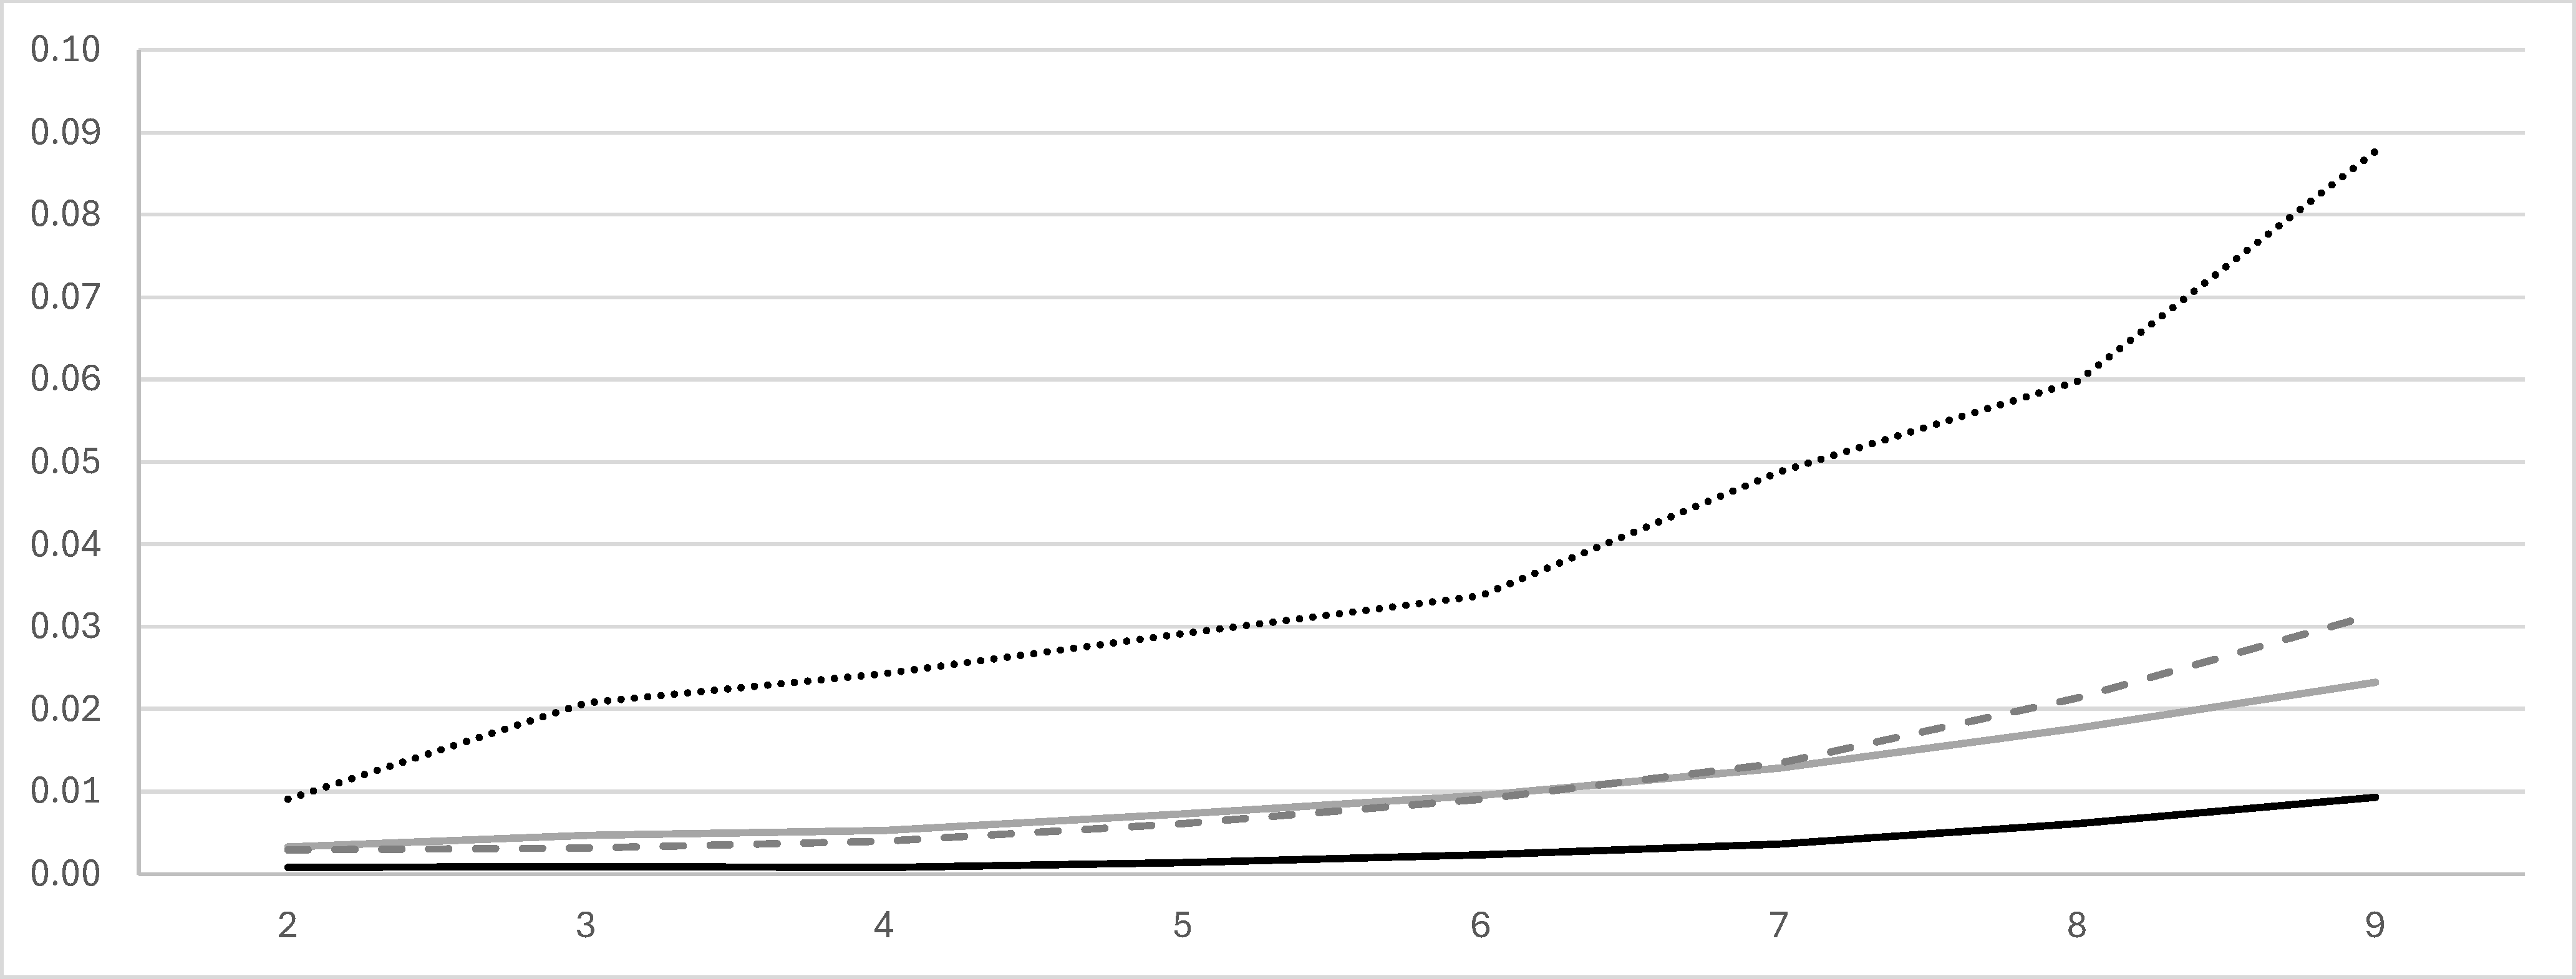
\includegraphics[width=\linewidth]{img/trend-emd-small.pdf}
	\captionof{figure}{\centering Trend Dimensi Metrik Sisi Graf Kecil}
\end{minipage}


	\vfill \vfill \vfill
\end{center}
\end{landscape}

\section{Pembahasan Hasil Eksekusi Graf Besar}
\label{sec:discussion-large}

Kedua, dibahas hasil eksekusi untuk graf besar. Berbeda dari evaluasi untuk graf kecil, pada graf besar ini setiap algoritma mengalami kegagalan dalam menentukan dimensi metrik maupun dimensi metrik sisi, karena melebihi batas waktu eksekusi. Hal ini tertera secara ringkas pada \autoref{tab:freq-fail-large}. Terlihat \autoref{alg:pseudo-boolean} mengalami kegagalan paling sedikit dalam menentukan dimensi metrik dan dimensi metrik sisi, sementara algoritma yang mengalami kegagalan paling banyak dalam menentukan dimensi metrik adalah \autoref{alg:boolean-satisfiability} dan dalam menentukan dimensi metrik sisi adalah \autoref{alg:brute-force}. Namun, kesimpulan ini tidak menggambarkan seluruh cerita, sehingga perlu dilihat rincian frekuensi lebih detail.

Untuk frekuensi dimensi metrik dari hasil eksekusi setiap algoritma dapat dilihat pada \autoref{tab:freq-md-large-bf}, \autoref{tab:freq-md-large-bs}, \autoref{tab:freq-md-large-lia}, dan \autoref{tab:freq-md-large-pb}. Terlihat bahwa untuk semua algoritma, penentuan dimensi metrik berhasil untuk seluruh graf dengan banyak simpul dari 10 hingga 40, dan semua algoritma menghasilkan frekuensi yang sama. Akan tetapi, \autoref{alg:brute-force}, \autoref{alg:boolean-satisfiability}, dan \autoref{alg:linear-integer-arithmetic}, baru mengalami kegagalan mulai dari graf dengan 45 simpul. Lebih kuat lagi, ketiga algoritma ini gagal dalam menentukan dimensi metrik untuk seluruh graf bersimpul 50. Di sisi lain, \autoref{alg:pseudo-boolean} adalah satu-satunya yang tidak mengalami kegagalan sama sekali dalam penentuan dimensi metrik graf besar.

Untuk frekuensi dimensi metrik sisi, hasil eksekusi setiap algoritma dapat dilihat pada \autoref{tab:freq-emd-large-bf}, \autoref{tab:freq-emd-large-bs}, \autoref{tab:freq-emd-large-lia}, dan \autoref{tab:freq-emd-large-pb}. \autoref{alg:brute-force} seluruhnya gagal menentukan dimensi metrik sisi sejak graf dengan 30 simpul. Sedangkan \autoref{alg:boolean-satisfiability} dan \autoref{alg:linear-integer-arithmetic} seluruhnya gagal sejak graf dengan 40 simpul. Sementara itu, \autoref{alg:pseudo-boolean} baru mulai seluruhnya gagal sejak graf dengan 45 simpul.

Seperti sebelumnya, rata-rata waktu eksekusi dihitung berdasarkan banyaknya simpul \(n\) frekuensi dimensi metrik atau dimensi metrik sisi terbanyak. Untuk graf besar bersimpul 10 hingga 45, frekuensi dimensi metrik terbanyak berturut-turut adalah 3, 4, 5, 5, 6, 6, 6, 6. Untuk graf besar bersimpul 10 hingga 35, frekuensi dimensi metrik sisi terbanyak berturut-turut adalah 5, 8, 10, 12, 14, 15. Hasil perhitungan rata-rata waktu eksekusi untuk dimensi metrik dapat dilihat pada \autoref{tab:mean-md-large}, dan untuk dimensi metrik sisi pada \autoref{tab:mean-emd-large}.

Demikian pula, rata-rata waktu eksekusi yang telah diperoleh untuk membandingkan waktu eksekusi antar algoritma dapat diilustrasikan lebih jelas sebagai grafik tren. Untuk dimensi metrik, dapat diamati pada \autoref{fig:trend-md-large}. Untuk dimensi metrik sisi, dapat diamati pada \autoref{fig:trend-emd-large}. Untuk grafik \autoref{fig:trend-emd-large} dipecah menjadi dua, karena rata-rata waktu eksekusi untuk \autoref{alg:brute-force} hanya tersedia hingga graf bersimpul 25, dan diilustrasikan sebagai (a). Kemudian, (b) melanjutkan perbandingan tren untuk \autoref{alg:boolean-satisfiability} dan \autoref{alg:pseudo-boolean} hingga graf bersimpul 35. Tren untuk \autoref{alg:linear-integer-arithmetic} tidak dimasukkan dalam (b) karena rata-rata waktu eksekusi hanya tersedia hingga graf bersimpul 30.

Dapat diamati, dalam menentukan dimensi metrik untuk graf bersimpul \(n\), seiring membesarnya \(n\), \autoref{alg:pseudo-boolean} adalah yang paling cepat. Sama pula, dalam menentukan dimensi metrik sisi, seiring membesarnya \(n\), \autoref{alg:pseudo-boolean} juga adalah yang paling cepat. Catat bahwa meskipun \autoref{fig:trend-emd-large} (b) menunjukkan \autoref{alg:boolean-satisfiability} dan \autoref{alg:pseudo-boolean} memiliki tren yang mirip, ini hanya ilustrasi parsial karena \autoref{alg:boolean-satisfiability} seluruhnya gagal pada graf bersimpul 40, sedangkan \autoref{alg:pseudo-boolean} masih berhasil.

\begin{landscape}
\begin{center}
	\renewcommand{\minipagewidth}{0.475\linewidth}

	\vphantom{}
	\vfill

	\begin{minipage}[\minipagealign]{\minipagewidth}
	\centering
	\captionof{table}{\centering Frekuensi Dimensi Metrik Graf Besar \foreign{Brute-force}}
	\resizetofit{
		\begin{tabular}{|c|lllllllll|}
			\hline \multirow{2}{*}{\begin{tabular}[c]{@{}c@{}}Dimensi\\ Metrik\end{tabular}} & \multicolumn{9}{c|}{Banyak Simpul} \\ \cline{2-10} & \multicolumn{1}{c|}{10} & \multicolumn{1}{c|}{15} & \multicolumn{1}{c|}{20} & \multicolumn{1}{c|}{25} & \multicolumn{1}{c|}{30} & \multicolumn{1}{c|}{35} & \multicolumn{1}{c|}{40} & \multicolumn{1}{c|}{45} & \multicolumn{1}{c|}{50} \\ \hline 2 & \multicolumn{1}{r|}{1} & \multicolumn{1}{r|}{} & \multicolumn{1}{r|}{} & \multicolumn{1}{r|}{} & \multicolumn{1}{r|}{} & \multicolumn{1}{r|}{} & \multicolumn{1}{r|}{} & \multicolumn{1}{r|}{} & \\ \hline 3 & \multicolumn{1}{r|}{34} & \multicolumn{1}{r|}{} & \multicolumn{1}{r|}{} & \multicolumn{1}{r|}{} & \multicolumn{1}{r|}{} & \multicolumn{1}{r|}{} & \multicolumn{1}{r|}{} & \multicolumn{1}{r|}{} & \\ \hline 4 & \multicolumn{1}{r|}{14} & \multicolumn{1}{r|}{50} & \multicolumn{1}{r|}{4} & \multicolumn{1}{r|}{} & \multicolumn{1}{r|}{} & \multicolumn{1}{r|}{} & \multicolumn{1}{r|}{} & \multicolumn{1}{r|}{} & \\ \hline 5 & \multicolumn{1}{r|}{1} & \multicolumn{1}{r|}{} & \multicolumn{1}{r|}{46} & \multicolumn{1}{r|}{50} & \multicolumn{1}{r|}{4} & \multicolumn{1}{r|}{} & \multicolumn{1}{r|}{} & \multicolumn{1}{r|}{} & \\ \hline 6 & \multicolumn{1}{r|}{} & \multicolumn{1}{r|}{} & \multicolumn{1}{r|}{} & \multicolumn{1}{r|}{} & \multicolumn{1}{r|}{46} & \multicolumn{1}{r|}{50} & \multicolumn{1}{r|}{50} & \multicolumn{1}{r|}{17} & \\ \hline 7 & \multicolumn{1}{r|}{} & \multicolumn{1}{r|}{} & \multicolumn{1}{r|}{} & \multicolumn{1}{r|}{} & \multicolumn{1}{r|}{} & \multicolumn{1}{r|}{} & \multicolumn{1}{r|}{} & \multicolumn{1}{r|}{} & \\ \hline Gagal & \multicolumn{1}{r|}{} & \multicolumn{1}{r|}{} & \multicolumn{1}{r|}{} & \multicolumn{1}{r|}{} & \multicolumn{1}{r|}{} & \multicolumn{1}{r|}{} & \multicolumn{1}{r|}{} & \multicolumn{1}{r|}{33} & 50 \\ \hline
		\end{tabular}
	}
\end{minipage}

	\hspace{2em}
	\begin{minipage}[\minipagealign]{\minipagewidth}
	\centering
	\captionof{table}{\centering Frekuensi Dimensi Metrik Graf Besar\\ \foreign{Boolean Satisfiability}}
	\resizetofit{
		\begin{tabular}{|c|lllllllll|}
			\hline \multirow{2}{*}{\begin{tabular}[c]{@{}c@{}}Dimensi\\ Metrik\end{tabular}} & \multicolumn{9}{c|}{Graf Bersimpul} \\ \cline{2-10} & \multicolumn{1}{c|}{10} & \multicolumn{1}{c|}{15} & \multicolumn{1}{c|}{20} & \multicolumn{1}{c|}{25} & \multicolumn{1}{c|}{30} & \multicolumn{1}{c|}{35} & \multicolumn{1}{c|}{40} & \multicolumn{1}{c|}{45} & \multicolumn{1}{c|}{50} \\ \hline 2 & \multicolumn{1}{r|}{1} & \multicolumn{1}{r|}{} & \multicolumn{1}{r|}{} & \multicolumn{1}{r|}{} & \multicolumn{1}{r|}{} & \multicolumn{1}{r|}{} & \multicolumn{1}{r|}{} & \multicolumn{1}{r|}{} & \\ \hline 3 & \multicolumn{1}{r|}{34} & \multicolumn{1}{r|}{} & \multicolumn{1}{r|}{} & \multicolumn{1}{r|}{} & \multicolumn{1}{r|}{} & \multicolumn{1}{r|}{} & \multicolumn{1}{r|}{} & \multicolumn{1}{r|}{} & \\ \hline 4 & \multicolumn{1}{r|}{14} & \multicolumn{1}{r|}{50} & \multicolumn{1}{r|}{4} & \multicolumn{1}{r|}{} & \multicolumn{1}{r|}{} & \multicolumn{1}{r|}{} & \multicolumn{1}{r|}{} & \multicolumn{1}{r|}{} & \\ \hline 5 & \multicolumn{1}{r|}{1} & \multicolumn{1}{r|}{} & \multicolumn{1}{r|}{46} & \multicolumn{1}{r|}{50} & \multicolumn{1}{r|}{4} & \multicolumn{1}{r|}{} & \multicolumn{1}{r|}{} & \multicolumn{1}{r|}{} & \\ \hline 6 & \multicolumn{1}{r|}{} & \multicolumn{1}{r|}{} & \multicolumn{1}{r|}{} & \multicolumn{1}{r|}{} & \multicolumn{1}{r|}{46} & \multicolumn{1}{r|}{50} & \multicolumn{1}{r|}{50} & \multicolumn{1}{r|}{14} & \\ \hline 7 & \multicolumn{1}{r|}{} & \multicolumn{1}{r|}{} & \multicolumn{1}{r|}{} & \multicolumn{1}{r|}{} & \multicolumn{1}{r|}{} & \multicolumn{1}{r|}{} & \multicolumn{1}{r|}{} & \multicolumn{1}{r|}{} & \\ \hline Gagal & \multicolumn{1}{r|}{} & \multicolumn{1}{r|}{} & \multicolumn{1}{r|}{} & \multicolumn{1}{r|}{} & \multicolumn{1}{r|}{} & \multicolumn{1}{r|}{} & \multicolumn{1}{r|}{} & \multicolumn{1}{r|}{36} & 50 \\ \hline
		\end{tabular}
	}
	\label{tab:freq-md-large-bs}
\end{minipage}


	\vspace{2em}

	\begin{minipage}[\minipagealign]{\minipagewidth}
	\centering
	\captionof{table}{\centering Frekuensi Dimensi Metrik Graf Besar \foreign{Linear Integer Arithmetic}}
	\resizetofit{
		\begin{tabular}{|c|lllllllll|}
			\hline \multirow{2}{*}{\begin{tabular}[c]{@{}c@{}}Dimensi\\ Metrik\end{tabular}} & \multicolumn{9}{c|}{Banyak Simpul} \\ \cline{2-10} & \multicolumn{1}{c|}{10} & \multicolumn{1}{c|}{15} & \multicolumn{1}{c|}{20} & \multicolumn{1}{c|}{25} & \multicolumn{1}{c|}{30} & \multicolumn{1}{c|}{35} & \multicolumn{1}{c|}{40} & \multicolumn{1}{c|}{45} & \multicolumn{1}{c|}{50} \\ \hline 2 & \multicolumn{1}{r|}{1} & \multicolumn{1}{r|}{} & \multicolumn{1}{r|}{} & \multicolumn{1}{r|}{} & \multicolumn{1}{r|}{} & \multicolumn{1}{r|}{} & \multicolumn{1}{r|}{} & \multicolumn{1}{r|}{} & \\ \hline 3 & \multicolumn{1}{r|}{34} & \multicolumn{1}{r|}{} & \multicolumn{1}{r|}{} & \multicolumn{1}{r|}{} & \multicolumn{1}{r|}{} & \multicolumn{1}{r|}{} & \multicolumn{1}{r|}{} & \multicolumn{1}{r|}{} & \\ \hline 4 & \multicolumn{1}{r|}{14} & \multicolumn{1}{r|}{50} & \multicolumn{1}{r|}{4} & \multicolumn{1}{r|}{} & \multicolumn{1}{r|}{} & \multicolumn{1}{r|}{} & \multicolumn{1}{r|}{} & \multicolumn{1}{r|}{} & \\ \hline 5 & \multicolumn{1}{r|}{1} & \multicolumn{1}{r|}{} & \multicolumn{1}{r|}{46} & \multicolumn{1}{r|}{50} & \multicolumn{1}{r|}{4} & \multicolumn{1}{r|}{} & \multicolumn{1}{r|}{} & \multicolumn{1}{r|}{} & \\ \hline 6 & \multicolumn{1}{r|}{} & \multicolumn{1}{r|}{} & \multicolumn{1}{r|}{} & \multicolumn{1}{r|}{} & \multicolumn{1}{r|}{46} & \multicolumn{1}{r|}{50} & \multicolumn{1}{r|}{50} & \multicolumn{1}{r|}{23} & \\ \hline 7 & \multicolumn{1}{r|}{} & \multicolumn{1}{r|}{} & \multicolumn{1}{r|}{} & \multicolumn{1}{r|}{} & \multicolumn{1}{r|}{} & \multicolumn{1}{r|}{} & \multicolumn{1}{r|}{} & \multicolumn{1}{r|}{} & \\ \hline Gagal & \multicolumn{1}{r|}{} & \multicolumn{1}{r|}{} & \multicolumn{1}{r|}{} & \multicolumn{1}{r|}{} & \multicolumn{1}{r|}{} & \multicolumn{1}{r|}{} & \multicolumn{1}{r|}{} & \multicolumn{1}{r|}{27} & 50 \\ \hline
		\end{tabular}
	}
\end{minipage}

	\hspace{2em}
	\begin{minipage}[\minipagealign]{\minipagewidth}
	\centering
	\captionof{table}{\centering Frekuensi Dimensi Metrik Graf Besar\\ \foreign{Pseudo Boolean}}
	\resizetofit{
		\begin{tabular}{|c|lllllllll|}
			\hline \multirow{2}{*}{\begin{tabular}[c]{@{}c@{}}Dimensi\\ Metrik\end{tabular}} & \multicolumn{9}{c|}{Graf Bersimpul} \\ \cline{2-10} & \multicolumn{1}{c|}{10} & \multicolumn{1}{c|}{15} & \multicolumn{1}{c|}{20} & \multicolumn{1}{c|}{25} & \multicolumn{1}{c|}{30} & \multicolumn{1}{c|}{35} & \multicolumn{1}{c|}{40} & \multicolumn{1}{c|}{45} & \multicolumn{1}{c|}{50} \\ \hline 2 & \multicolumn{1}{r|}{1} & \multicolumn{1}{r|}{} & \multicolumn{1}{r|}{} & \multicolumn{1}{r|}{} & \multicolumn{1}{r|}{} & \multicolumn{1}{r|}{} & \multicolumn{1}{r|}{} & \multicolumn{1}{r|}{} & \\ \hline 3 & \multicolumn{1}{r|}{34} & \multicolumn{1}{r|}{} & \multicolumn{1}{r|}{} & \multicolumn{1}{r|}{} & \multicolumn{1}{r|}{} & \multicolumn{1}{r|}{} & \multicolumn{1}{r|}{} & \multicolumn{1}{r|}{} & \\ \hline 4 & \multicolumn{1}{r|}{14} & \multicolumn{1}{r|}{50} & \multicolumn{1}{r|}{4} & \multicolumn{1}{r|}{} & \multicolumn{1}{r|}{} & \multicolumn{1}{r|}{} & \multicolumn{1}{r|}{} & \multicolumn{1}{r|}{} & \\ \hline 5 & \multicolumn{1}{r|}{1} & \multicolumn{1}{r|}{} & \multicolumn{1}{r|}{46} & \multicolumn{1}{r|}{50} & \multicolumn{1}{r|}{4} & \multicolumn{1}{r|}{} & \multicolumn{1}{r|}{} & \multicolumn{1}{r|}{} & \\ \hline 6 & \multicolumn{1}{r|}{} & \multicolumn{1}{r|}{} & \multicolumn{1}{r|}{} & \multicolumn{1}{r|}{} & \multicolumn{1}{r|}{46} & \multicolumn{1}{r|}{50} & \multicolumn{1}{r|}{50} & \multicolumn{1}{r|}{39} & 1 \\ \hline 7 & \multicolumn{1}{r|}{} & \multicolumn{1}{r|}{} & \multicolumn{1}{r|}{} & \multicolumn{1}{r|}{} & \multicolumn{1}{r|}{} & \multicolumn{1}{r|}{} & \multicolumn{1}{r|}{} & \multicolumn{1}{r|}{11} & 49 \\ \hline Gagal & \multicolumn{1}{r|}{} & \multicolumn{1}{r|}{} & \multicolumn{1}{r|}{} & \multicolumn{1}{r|}{} & \multicolumn{1}{r|}{} & \multicolumn{1}{r|}{} & \multicolumn{1}{r|}{} & \multicolumn{1}{r|}{} & \\ \hline
		\end{tabular}
	}
\end{minipage}


	\vfill \vfill \vfill
\end{center}
\end{landscape}

\begin{center}
	\renewcommand{\minipagewidth}{0.475\linewidth}

	\vphantom{}
	\vfill

	\begin{minipage}[\minipagealign]{\minipagewidth}
	\centering
	\captionof{table}{\centering Frekuensi Dimensi Metrik Sisi Graf Besar \foreign{Brute-force}}
	\resizetofit{
		\begin{tabular}{|c|lllllllll|}
			\hline \multirow{2}{*}{\begin{tabular}[c]{@{}c@{}}Dimensi\\ Metrik Sisi\end{tabular}} & \multicolumn{9}{c|}{Graf Bersimpul} \\ \cline{2-10} & \multicolumn{1}{c|}{10} & \multicolumn{1}{c|}{15} & \multicolumn{1}{c|}{20} & \multicolumn{1}{c|}{25} & \multicolumn{1}{c|}{30} & \multicolumn{1}{c|}{35} & \multicolumn{1}{c|}{40} & \multicolumn{1}{c|}{45} & \multicolumn{1}{c|}{50} \\ \hline 4 & \multicolumn{1}{r|}{6} & \multicolumn{1}{r|}{} & \multicolumn{1}{r|}{} & \multicolumn{1}{r|}{} & \multicolumn{1}{r|}{} & \multicolumn{1}{r|}{} & \multicolumn{1}{r|}{} & \multicolumn{1}{r|}{} & \\ \hline 5 & \multicolumn{1}{r|}{27} & \multicolumn{1}{r|}{} & \multicolumn{1}{r|}{} & \multicolumn{1}{r|}{} & \multicolumn{1}{r|}{} & \multicolumn{1}{r|}{} & \multicolumn{1}{r|}{} & \multicolumn{1}{r|}{} & \\ \hline 6 & \multicolumn{1}{r|}{13} & \multicolumn{1}{r|}{} & \multicolumn{1}{r|}{} & \multicolumn{1}{r|}{} & \multicolumn{1}{r|}{} & \multicolumn{1}{r|}{} & \multicolumn{1}{r|}{} & \multicolumn{1}{r|}{} & \\ \hline 7 & \multicolumn{1}{r|}{4} & \multicolumn{1}{r|}{11} & \multicolumn{1}{r|}{} & \multicolumn{1}{r|}{} & \multicolumn{1}{r|}{} & \multicolumn{1}{r|}{} & \multicolumn{1}{r|}{} & \multicolumn{1}{r|}{} & \\ \hline 8 & \multicolumn{1}{r|}{} & \multicolumn{1}{r|}{19} & \multicolumn{1}{r|}{} & \multicolumn{1}{r|}{} & \multicolumn{1}{r|}{} & \multicolumn{1}{r|}{} & \multicolumn{1}{r|}{} & \multicolumn{1}{r|}{} & \\ \hline 9 & \multicolumn{1}{r|}{} & \multicolumn{1}{r|}{13} & \multicolumn{1}{r|}{10} & \multicolumn{1}{r|}{} & \multicolumn{1}{r|}{} & \multicolumn{1}{r|}{} & \multicolumn{1}{r|}{} & \multicolumn{1}{r|}{} & \\ \hline 10 & \multicolumn{1}{r|}{} & \multicolumn{1}{r|}{6} & \multicolumn{1}{r|}{19} & \multicolumn{1}{r|}{2} & \multicolumn{1}{r|}{} & \multicolumn{1}{r|}{} & \multicolumn{1}{r|}{} & \multicolumn{1}{r|}{} & \\ \hline 11 & \multicolumn{1}{r|}{} & \multicolumn{1}{r|}{1} & \multicolumn{1}{r|}{10} & \multicolumn{1}{r|}{7} & \multicolumn{1}{r|}{} & \multicolumn{1}{r|}{} & \multicolumn{1}{r|}{} & \multicolumn{1}{r|}{} & \\ \hline 12 & \multicolumn{1}{r|}{} & \multicolumn{1}{r|}{} & \multicolumn{1}{r|}{10} & \multicolumn{1}{r|}{25} & \multicolumn{1}{r|}{} & \multicolumn{1}{r|}{} & \multicolumn{1}{r|}{} & \multicolumn{1}{r|}{} & \\ \hline 13 & \multicolumn{1}{r|}{} & \multicolumn{1}{r|}{} & \multicolumn{1}{r|}{} & \multicolumn{1}{r|}{13} & \multicolumn{1}{r|}{} & \multicolumn{1}{r|}{} & \multicolumn{1}{r|}{} & \multicolumn{1}{r|}{} & \\ \hline 14 & \multicolumn{1}{r|}{} & \multicolumn{1}{r|}{} & \multicolumn{1}{r|}{1} & \multicolumn{1}{r|}{1} & \multicolumn{1}{r|}{} & \multicolumn{1}{r|}{} & \multicolumn{1}{r|}{} & \multicolumn{1}{r|}{} & \\ \hline 15 & \multicolumn{1}{r|}{} & \multicolumn{1}{r|}{} & \multicolumn{1}{r|}{} & \multicolumn{1}{r|}{1} & \multicolumn{1}{r|}{} & \multicolumn{1}{r|}{} & \multicolumn{1}{r|}{} & \multicolumn{1}{r|}{} & \\ \hline 16 & \multicolumn{1}{r|}{} & \multicolumn{1}{r|}{} & \multicolumn{1}{r|}{} & \multicolumn{1}{r|}{} & \multicolumn{1}{r|}{} & \multicolumn{1}{r|}{} & \multicolumn{1}{r|}{} & \multicolumn{1}{r|}{} & \\ \hline 17 & \multicolumn{1}{r|}{} & \multicolumn{1}{r|}{} & \multicolumn{1}{r|}{} & \multicolumn{1}{r|}{} & \multicolumn{1}{r|}{} & \multicolumn{1}{r|}{} & \multicolumn{1}{r|}{} & \multicolumn{1}{r|}{} & \\ \hline 18 & \multicolumn{1}{r|}{} & \multicolumn{1}{r|}{} & \multicolumn{1}{r|}{} & \multicolumn{1}{r|}{} & \multicolumn{1}{r|}{} & \multicolumn{1}{r|}{} & \multicolumn{1}{r|}{} & \multicolumn{1}{r|}{} & \\ \hline Gagal & \multicolumn{1}{r|}{} & \multicolumn{1}{r|}{} & \multicolumn{1}{r|}{} & \multicolumn{1}{r|}{1} & \multicolumn{1}{r|}{50} & \multicolumn{1}{r|}{50} & \multicolumn{1}{r|}{50} & \multicolumn{1}{r|}{50} & 50 \\ \hline
		\end{tabular}
	}
	\label{tab:freq-emd-large-bs}
\end{minipage}

	\hspace{1em}
	\begin{minipage}[\minipagealign]{\minipagewidth}
	\centering
	\captionof{table}{\centering Frekuensi Dimensi Metrik Sisi Graf Besar \foreign{Boolean Satisfiability}}
	\resizetofit{
		\begin{tabular}{|c|lllllllll|}
			\hline \multirow{2}{*}{\begin{tabular}[c]{@{}c@{}}Dimensi\\ Metrik Sisi\end{tabular}} & \multicolumn{9}{c|}{Graf Bersimpul} \\ \cline{2-10} & \multicolumn{1}{c|}{10} & \multicolumn{1}{c|}{15} & \multicolumn{1}{c|}{20} & \multicolumn{1}{c|}{25} & \multicolumn{1}{c|}{30} & \multicolumn{1}{c|}{35} & \multicolumn{1}{c|}{40} & \multicolumn{1}{c|}{45} & \multicolumn{1}{c|}{50} \\ \hline 4 & \multicolumn{1}{r|}{6} & \multicolumn{1}{r|}{} & \multicolumn{1}{r|}{} & \multicolumn{1}{r|}{} & \multicolumn{1}{r|}{} & \multicolumn{1}{r|}{} & \multicolumn{1}{r|}{} & \multicolumn{1}{r|}{} & \\ \hline 5 & \multicolumn{1}{r|}{27} & \multicolumn{1}{r|}{} & \multicolumn{1}{r|}{} & \multicolumn{1}{r|}{} & \multicolumn{1}{r|}{} & \multicolumn{1}{r|}{} & \multicolumn{1}{r|}{} & \multicolumn{1}{r|}{} & \\ \hline 6 & \multicolumn{1}{r|}{13} & \multicolumn{1}{r|}{} & \multicolumn{1}{r|}{} & \multicolumn{1}{r|}{} & \multicolumn{1}{r|}{} & \multicolumn{1}{r|}{} & \multicolumn{1}{r|}{} & \multicolumn{1}{r|}{} & \\ \hline 7 & \multicolumn{1}{r|}{4} & \multicolumn{1}{r|}{11} & \multicolumn{1}{r|}{} & \multicolumn{1}{r|}{} & \multicolumn{1}{r|}{} & \multicolumn{1}{r|}{} & \multicolumn{1}{r|}{} & \multicolumn{1}{r|}{} & \\ \hline 8 & \multicolumn{1}{r|}{} & \multicolumn{1}{r|}{19} & \multicolumn{1}{r|}{} & \multicolumn{1}{r|}{} & \multicolumn{1}{r|}{} & \multicolumn{1}{r|}{} & \multicolumn{1}{r|}{} & \multicolumn{1}{r|}{} & \\ \hline 9 & \multicolumn{1}{r|}{} & \multicolumn{1}{r|}{13} & \multicolumn{1}{r|}{10} & \multicolumn{1}{r|}{} & \multicolumn{1}{r|}{} & \multicolumn{1}{r|}{} & \multicolumn{1}{r|}{} & \multicolumn{1}{r|}{} & \\ \hline 10 & \multicolumn{1}{r|}{} & \multicolumn{1}{r|}{6} & \multicolumn{1}{r|}{19} & \multicolumn{1}{r|}{2} & \multicolumn{1}{r|}{} & \multicolumn{1}{r|}{} & \multicolumn{1}{r|}{} & \multicolumn{1}{r|}{} & \\ \hline 11 & \multicolumn{1}{r|}{} & \multicolumn{1}{r|}{1} & \multicolumn{1}{r|}{10} & \multicolumn{1}{r|}{7} & \multicolumn{1}{r|}{} & \multicolumn{1}{r|}{} & \multicolumn{1}{r|}{} & \multicolumn{1}{r|}{} & \\ \hline 12 & \multicolumn{1}{r|}{} & \multicolumn{1}{r|}{} & \multicolumn{1}{r|}{10} & \multicolumn{1}{r|}{26} & \multicolumn{1}{r|}{3} & \multicolumn{1}{r|}{} & \multicolumn{1}{r|}{} & \multicolumn{1}{r|}{} & \\ \hline 13 & \multicolumn{1}{r|}{} & \multicolumn{1}{r|}{} & \multicolumn{1}{r|}{} & \multicolumn{1}{r|}{13} & \multicolumn{1}{r|}{16} & \multicolumn{1}{r|}{} & \multicolumn{1}{r|}{} & \multicolumn{1}{r|}{} & \\ \hline 14 & \multicolumn{1}{r|}{} & \multicolumn{1}{r|}{} & \multicolumn{1}{r|}{1} & \multicolumn{1}{r|}{1} & \multicolumn{1}{r|}{26} & \multicolumn{1}{r|}{1} & \multicolumn{1}{r|}{} & \multicolumn{1}{r|}{} & \\ \hline 15 & \multicolumn{1}{r|}{} & \multicolumn{1}{r|}{} & \multicolumn{1}{r|}{} & \multicolumn{1}{r|}{1} & \multicolumn{1}{r|}{4} & \multicolumn{1}{r|}{3} & \multicolumn{1}{r|}{} & \multicolumn{1}{r|}{} & \\ \hline 16 & \multicolumn{1}{r|}{} & \multicolumn{1}{r|}{} & \multicolumn{1}{r|}{} & \multicolumn{1}{r|}{} & \multicolumn{1}{r|}{} & \multicolumn{1}{r|}{1} & \multicolumn{1}{r|}{} & \multicolumn{1}{r|}{} & \\ \hline 17 & \multicolumn{1}{r|}{} & \multicolumn{1}{r|}{} & \multicolumn{1}{r|}{} & \multicolumn{1}{r|}{} & \multicolumn{1}{r|}{} & \multicolumn{1}{r|}{} & \multicolumn{1}{r|}{} & \multicolumn{1}{r|}{} & \\ \hline 18 & \multicolumn{1}{r|}{} & \multicolumn{1}{r|}{} & \multicolumn{1}{r|}{} & \multicolumn{1}{r|}{} & \multicolumn{1}{r|}{} & \multicolumn{1}{r|}{1} & \multicolumn{1}{r|}{} & \multicolumn{1}{r|}{} & \\ \hline Gagal & \multicolumn{1}{r|}{} & \multicolumn{1}{r|}{} & \multicolumn{1}{r|}{} & \multicolumn{1}{r|}{} & \multicolumn{1}{r|}{1} & \multicolumn{1}{r|}{44} & \multicolumn{1}{r|}{50} & \multicolumn{1}{r|}{50} & 50 \\ \hline
		\end{tabular}
	}
	\label{tab:freq-emd-large-bf}
\end{minipage}


	\vspace{2em}

	\begin{minipage}[\minipagealign]{\minipagewidth}
	\centering
	\captionof{table}{\centering Frekuensi Dimensi Metrik Sisi Graf Besar \foreign{Linear Integer Arithmetic}}
	\resizetofit{
		\begin{tabular}{|c|lllllllll|}
			\hline \multirow{2}{*}{\begin{tabular}[c]{@{}c@{}}Dimensi\\ Metrik Sisi\end{tabular}} & \multicolumn{9}{c|}{Graf Bersimpul} \\ \cline{2-10} & \multicolumn{1}{c|}{10} & \multicolumn{1}{c|}{15} & \multicolumn{1}{c|}{20} & \multicolumn{1}{c|}{25} & \multicolumn{1}{c|}{30} & \multicolumn{1}{c|}{35} & \multicolumn{1}{c|}{40} & \multicolumn{1}{c|}{45} & \multicolumn{1}{c|}{50} \\ \hline 4 & \multicolumn{1}{r|}{6} & \multicolumn{1}{r|}{} & \multicolumn{1}{r|}{} & \multicolumn{1}{r|}{} & \multicolumn{1}{r|}{} & \multicolumn{1}{r|}{} & \multicolumn{1}{r|}{} & \multicolumn{1}{r|}{} & \\ \hline 5 & \multicolumn{1}{r|}{27} & \multicolumn{1}{r|}{} & \multicolumn{1}{r|}{} & \multicolumn{1}{r|}{} & \multicolumn{1}{r|}{} & \multicolumn{1}{r|}{} & \multicolumn{1}{r|}{} & \multicolumn{1}{r|}{} & \\ \hline 6 & \multicolumn{1}{r|}{13} & \multicolumn{1}{r|}{} & \multicolumn{1}{r|}{} & \multicolumn{1}{r|}{} & \multicolumn{1}{r|}{} & \multicolumn{1}{r|}{} & \multicolumn{1}{r|}{} & \multicolumn{1}{r|}{} & \\ \hline 7 & \multicolumn{1}{r|}{4} & \multicolumn{1}{r|}{11} & \multicolumn{1}{r|}{} & \multicolumn{1}{r|}{} & \multicolumn{1}{r|}{} & \multicolumn{1}{r|}{} & \multicolumn{1}{r|}{} & \multicolumn{1}{r|}{} & \\ \hline 8 & \multicolumn{1}{r|}{} & \multicolumn{1}{r|}{19} & \multicolumn{1}{r|}{} & \multicolumn{1}{r|}{} & \multicolumn{1}{r|}{} & \multicolumn{1}{r|}{} & \multicolumn{1}{r|}{} & \multicolumn{1}{r|}{} & \\ \hline 9 & \multicolumn{1}{r|}{} & \multicolumn{1}{r|}{13} & \multicolumn{1}{r|}{10} & \multicolumn{1}{r|}{} & \multicolumn{1}{r|}{} & \multicolumn{1}{r|}{} & \multicolumn{1}{r|}{} & \multicolumn{1}{r|}{} & \\ \hline 10 & \multicolumn{1}{r|}{} & \multicolumn{1}{r|}{6} & \multicolumn{1}{r|}{19} & \multicolumn{1}{r|}{2} & \multicolumn{1}{r|}{} & \multicolumn{1}{r|}{} & \multicolumn{1}{r|}{} & \multicolumn{1}{r|}{} & \\ \hline 11 & \multicolumn{1}{r|}{} & \multicolumn{1}{r|}{1} & \multicolumn{1}{r|}{10} & \multicolumn{1}{r|}{7} & \multicolumn{1}{r|}{} & \multicolumn{1}{r|}{} & \multicolumn{1}{r|}{} & \multicolumn{1}{r|}{} & \\ \hline 12 & \multicolumn{1}{r|}{} & \multicolumn{1}{r|}{} & \multicolumn{1}{r|}{10} & \multicolumn{1}{r|}{26} & \multicolumn{1}{r|}{2} & \multicolumn{1}{r|}{} & \multicolumn{1}{r|}{} & \multicolumn{1}{r|}{} & \\ \hline 13 & \multicolumn{1}{r|}{} & \multicolumn{1}{r|}{} & \multicolumn{1}{r|}{} & \multicolumn{1}{r|}{13} & \multicolumn{1}{r|}{14} & \multicolumn{1}{r|}{} & \multicolumn{1}{r|}{} & \multicolumn{1}{r|}{} & \\ \hline 14 & \multicolumn{1}{r|}{} & \multicolumn{1}{r|}{} & \multicolumn{1}{r|}{1} & \multicolumn{1}{r|}{1} & \multicolumn{1}{r|}{24} & \multicolumn{1}{r|}{1} & \multicolumn{1}{r|}{} & \multicolumn{1}{r|}{} & \\ \hline 15 & \multicolumn{1}{r|}{} & \multicolumn{1}{r|}{} & \multicolumn{1}{r|}{} & \multicolumn{1}{r|}{1} & \multicolumn{1}{r|}{4} & \multicolumn{1}{r|}{} & \multicolumn{1}{r|}{} & \multicolumn{1}{r|}{} & \\ \hline 16 & \multicolumn{1}{r|}{} & \multicolumn{1}{r|}{} & \multicolumn{1}{r|}{} & \multicolumn{1}{r|}{} & \multicolumn{1}{r|}{} & \multicolumn{1}{r|}{} & \multicolumn{1}{r|}{} & \multicolumn{1}{r|}{} & \\ \hline 17 & \multicolumn{1}{r|}{} & \multicolumn{1}{r|}{} & \multicolumn{1}{r|}{} & \multicolumn{1}{r|}{} & \multicolumn{1}{r|}{} & \multicolumn{1}{r|}{} & \multicolumn{1}{r|}{} & \multicolumn{1}{r|}{} & \\ \hline 18 & \multicolumn{1}{r|}{} & \multicolumn{1}{r|}{} & \multicolumn{1}{r|}{} & \multicolumn{1}{r|}{} & \multicolumn{1}{r|}{} & \multicolumn{1}{r|}{1} & \multicolumn{1}{r|}{} & \multicolumn{1}{r|}{} & \\ \hline Gagal & \multicolumn{1}{r|}{} & \multicolumn{1}{r|}{} & \multicolumn{1}{r|}{} & \multicolumn{1}{r|}{} & \multicolumn{1}{r|}{6} & \multicolumn{1}{r|}{48} & \multicolumn{1}{r|}{50} & \multicolumn{1}{r|}{50} & 50 \\ \hline
		\end{tabular}
	}
	\label{tab:freq-emd-large-lia}
\end{minipage}

	\hspace{1em}
	\begin{minipage}[\minipagealign]{\minipagewidth}
	\centering
	\captionof{table}{\centering Frekuensi Dimensi Metrik Sisi Graf Besar \foreign{Pseudo Boolean}}
	\resizetofit{
		\begin{tabular}{|c|lllllllll|}
			\hline \multirow{2}{*}{\begin{tabular}[c]{@{}c@{}}Dimensi\\ Metrik Sisi\end{tabular}} & \multicolumn{9}{c|}{Graf Bersimpul} \\ \cline{2-10} & \multicolumn{1}{c|}{10} & \multicolumn{1}{c|}{15} & \multicolumn{1}{c|}{20} & \multicolumn{1}{c|}{25} & \multicolumn{1}{c|}{30} & \multicolumn{1}{c|}{35} & \multicolumn{1}{c|}{40} & \multicolumn{1}{c|}{45} & \multicolumn{1}{c|}{50} \\ \hline 4 & \multicolumn{1}{r|}{6} & \multicolumn{1}{r|}{} & \multicolumn{1}{r|}{} & \multicolumn{1}{r|}{} & \multicolumn{1}{r|}{} & \multicolumn{1}{r|}{} & \multicolumn{1}{r|}{} & \multicolumn{1}{r|}{} & \\ \hline 5 & \multicolumn{1}{r|}{27} & \multicolumn{1}{r|}{} & \multicolumn{1}{r|}{} & \multicolumn{1}{r|}{} & \multicolumn{1}{r|}{} & \multicolumn{1}{r|}{} & \multicolumn{1}{r|}{} & \multicolumn{1}{r|}{} & \\ \hline 6 & \multicolumn{1}{r|}{13} & \multicolumn{1}{r|}{} & \multicolumn{1}{r|}{} & \multicolumn{1}{r|}{} & \multicolumn{1}{r|}{} & \multicolumn{1}{r|}{} & \multicolumn{1}{r|}{} & \multicolumn{1}{r|}{} & \\ \hline 7 & \multicolumn{1}{r|}{4} & \multicolumn{1}{r|}{11} & \multicolumn{1}{r|}{} & \multicolumn{1}{r|}{} & \multicolumn{1}{r|}{} & \multicolumn{1}{r|}{} & \multicolumn{1}{r|}{} & \multicolumn{1}{r|}{} & \\ \hline 8 & \multicolumn{1}{r|}{} & \multicolumn{1}{r|}{19} & \multicolumn{1}{r|}{} & \multicolumn{1}{r|}{} & \multicolumn{1}{r|}{} & \multicolumn{1}{r|}{} & \multicolumn{1}{r|}{} & \multicolumn{1}{r|}{} & \\ \hline 9 & \multicolumn{1}{r|}{} & \multicolumn{1}{r|}{13} & \multicolumn{1}{r|}{10} & \multicolumn{1}{r|}{} & \multicolumn{1}{r|}{} & \multicolumn{1}{r|}{} & \multicolumn{1}{r|}{} & \multicolumn{1}{r|}{} & \\ \hline 10 & \multicolumn{1}{r|}{} & \multicolumn{1}{r|}{6} & \multicolumn{1}{r|}{19} & \multicolumn{1}{r|}{2} & \multicolumn{1}{r|}{} & \multicolumn{1}{r|}{} & \multicolumn{1}{r|}{} & \multicolumn{1}{r|}{} & \\ \hline 11 & \multicolumn{1}{r|}{} & \multicolumn{1}{r|}{1} & \multicolumn{1}{r|}{10} & \multicolumn{1}{r|}{7} & \multicolumn{1}{r|}{} & \multicolumn{1}{r|}{} & \multicolumn{1}{r|}{} & \multicolumn{1}{r|}{} & \\ \hline 12 & \multicolumn{1}{r|}{} & \multicolumn{1}{r|}{} & \multicolumn{1}{r|}{10} & \multicolumn{1}{r|}{26} & \multicolumn{1}{r|}{4} & \multicolumn{1}{r|}{} & \multicolumn{1}{r|}{} & \multicolumn{1}{r|}{} & \\ \hline 13 & \multicolumn{1}{r|}{} & \multicolumn{1}{r|}{} & \multicolumn{1}{r|}{} & \multicolumn{1}{r|}{13} & \multicolumn{1}{r|}{16} & \multicolumn{1}{r|}{} & \multicolumn{1}{r|}{} & \multicolumn{1}{r|}{} & \\ \hline 14 & \multicolumn{1}{r|}{} & \multicolumn{1}{r|}{} & \multicolumn{1}{r|}{1} & \multicolumn{1}{r|}{1} & \multicolumn{1}{r|}{26} & \multicolumn{1}{r|}{10} & \multicolumn{1}{r|}{} & \multicolumn{1}{r|}{} & \\ \hline 15 & \multicolumn{1}{r|}{} & \multicolumn{1}{r|}{} & \multicolumn{1}{r|}{} & \multicolumn{1}{r|}{1} & \multicolumn{1}{r|}{4} & \multicolumn{1}{r|}{18} & \multicolumn{1}{r|}{} & \multicolumn{1}{r|}{} & \\ \hline 16 & \multicolumn{1}{r|}{} & \multicolumn{1}{r|}{} & \multicolumn{1}{r|}{} & \multicolumn{1}{r|}{} & \multicolumn{1}{r|}{} & \multicolumn{1}{r|}{9} & \multicolumn{1}{r|}{1} & \multicolumn{1}{r|}{} & \\ \hline 17 & \multicolumn{1}{r|}{} & \multicolumn{1}{r|}{} & \multicolumn{1}{r|}{} & \multicolumn{1}{r|}{} & \multicolumn{1}{r|}{} & \multicolumn{1}{r|}{2} & \multicolumn{1}{r|}{} & \multicolumn{1}{r|}{} & \\ \hline 18 & \multicolumn{1}{r|}{} & \multicolumn{1}{r|}{} & \multicolumn{1}{r|}{} & \multicolumn{1}{r|}{} & \multicolumn{1}{r|}{} & \multicolumn{1}{r|}{1} & \multicolumn{1}{r|}{} & \multicolumn{1}{r|}{} & \\ \hline Gagal & \multicolumn{1}{r|}{} & \multicolumn{1}{r|}{} & \multicolumn{1}{r|}{} & \multicolumn{1}{r|}{} & \multicolumn{1}{r|}{} & \multicolumn{1}{r|}{10} & \multicolumn{1}{r|}{49} & \multicolumn{1}{r|}{50} & 50 \\ \hline
		\end{tabular}
	}
\end{minipage}


	\vspace{2em}

	\renewcommand{\minipagewidth}{\linewidth}
	\begin{minipage}[\minipagealign]{\minipagewidth}
	\centering
	\captionof{table}{\centering Frekuensi Gagal Graf Besar}
	\resizetofit{
		\begin{tabular}{l|c|c|ll}
			\cline{2-3} & \multicolumn{1}{r|}{Dimensi Metrik} & \multicolumn{1}{r|}{Dimensi Metrik Sisi} & & \\ \cline{1-3} \multicolumn{1}{|l|}{\foreign{Brute-force}} & 83 & 251 & & \\ \cline{1-3} \multicolumn{1}{|l|}{\foreign{Boolean Satisfiability}} & 86 & 195 & & \\ \cline{1-3} \multicolumn{1}{|l|}{\foreign{Linear Integer Arithmetic}} & 77 & 204 & & \\ \cline{1-3} \multicolumn{1}{|l|}{\foreign{Pseudo Boolean}} & 0 & 159 & & \\ \cline{1-3}
		\end{tabular}
	}
	\label{tab:freq-fail-large}
\end{minipage}


	\vfill \vfill \vfill
\end{center}

\begin{landscape}
\begin{center}
	\renewcommand{\minipagewidth}{0.475\linewidth}

	\vphantom{}
	\vfill

	\begin{minipage}[\minipagealign]{\minipagewidth}
	\centering
	\captionof{table}{\centering Rata-Rata Waktu Eksekusi\\ Dimensi Metrik Graf Besar}
	\resizetofit{
		\begin{tabular}{|c|c|r|r|r|r|}
			\hline \begin{tabular}[c]{@{}c@{}}Dimensi\\ Metrik\end{tabular} & \begin{tabular}[c]{@{}c@{}}Banyak\\ Simpul\end{tabular} & \multicolumn{1}{c|}{\foreign{Brute-force}} & \multicolumn{1}{c|}{\begin{tabular}[c]{@{}c@{}}\foreign{Boolean}\\ \foreign{Satisfiability}\end{tabular}} & \multicolumn{1}{c|}{\begin{tabular}[c]{@{}c@{}}\foreign{Linear Integer}\\ \foreign{Arithmetic}\end{tabular}} & \multicolumn{1}{c|}{\begin{tabular}[c]{@{}c@{}}\foreign{Pseudo}\\ \foreign{Boolean}\end{tabular}} \\ \hline 3 & 10 & .004119 & .020946 & .115585 & .027161 \\ \hline 4 & 15 & .019737 & .072151 & .391855 & .155409 \\ \hline 5 & 20 & .131515 & .197247 & 1.306162 & .526939 \\ \hline 5 & 25 & .779308 & .474250 & 4.026042 & 1.523069 \\ \hline 6 & 30 & 4.967965 & 4.721401 & 11.883957 & 3.081103 \\ \hline 6 & 35 & 16.766268 & 20.284314 & 50.562551 & 6.585125 \\ \hline 6 & 40 & 71.217442 & 100.421604 & 204.669259 & 17.266515 \\ \hline 6 & 45 & 280.950692 & 438.786140 & 476.961207 & 64.249163 \\ \hline 7 & 50 & & & & 134.408767 \\ \hline
		\end{tabular}
	}
	\label{tab:mean-md-large}
\end{minipage}

	\hspace{2em}
	\begin{minipage}[\minipagealign]{\minipagewidth}
	\centering
	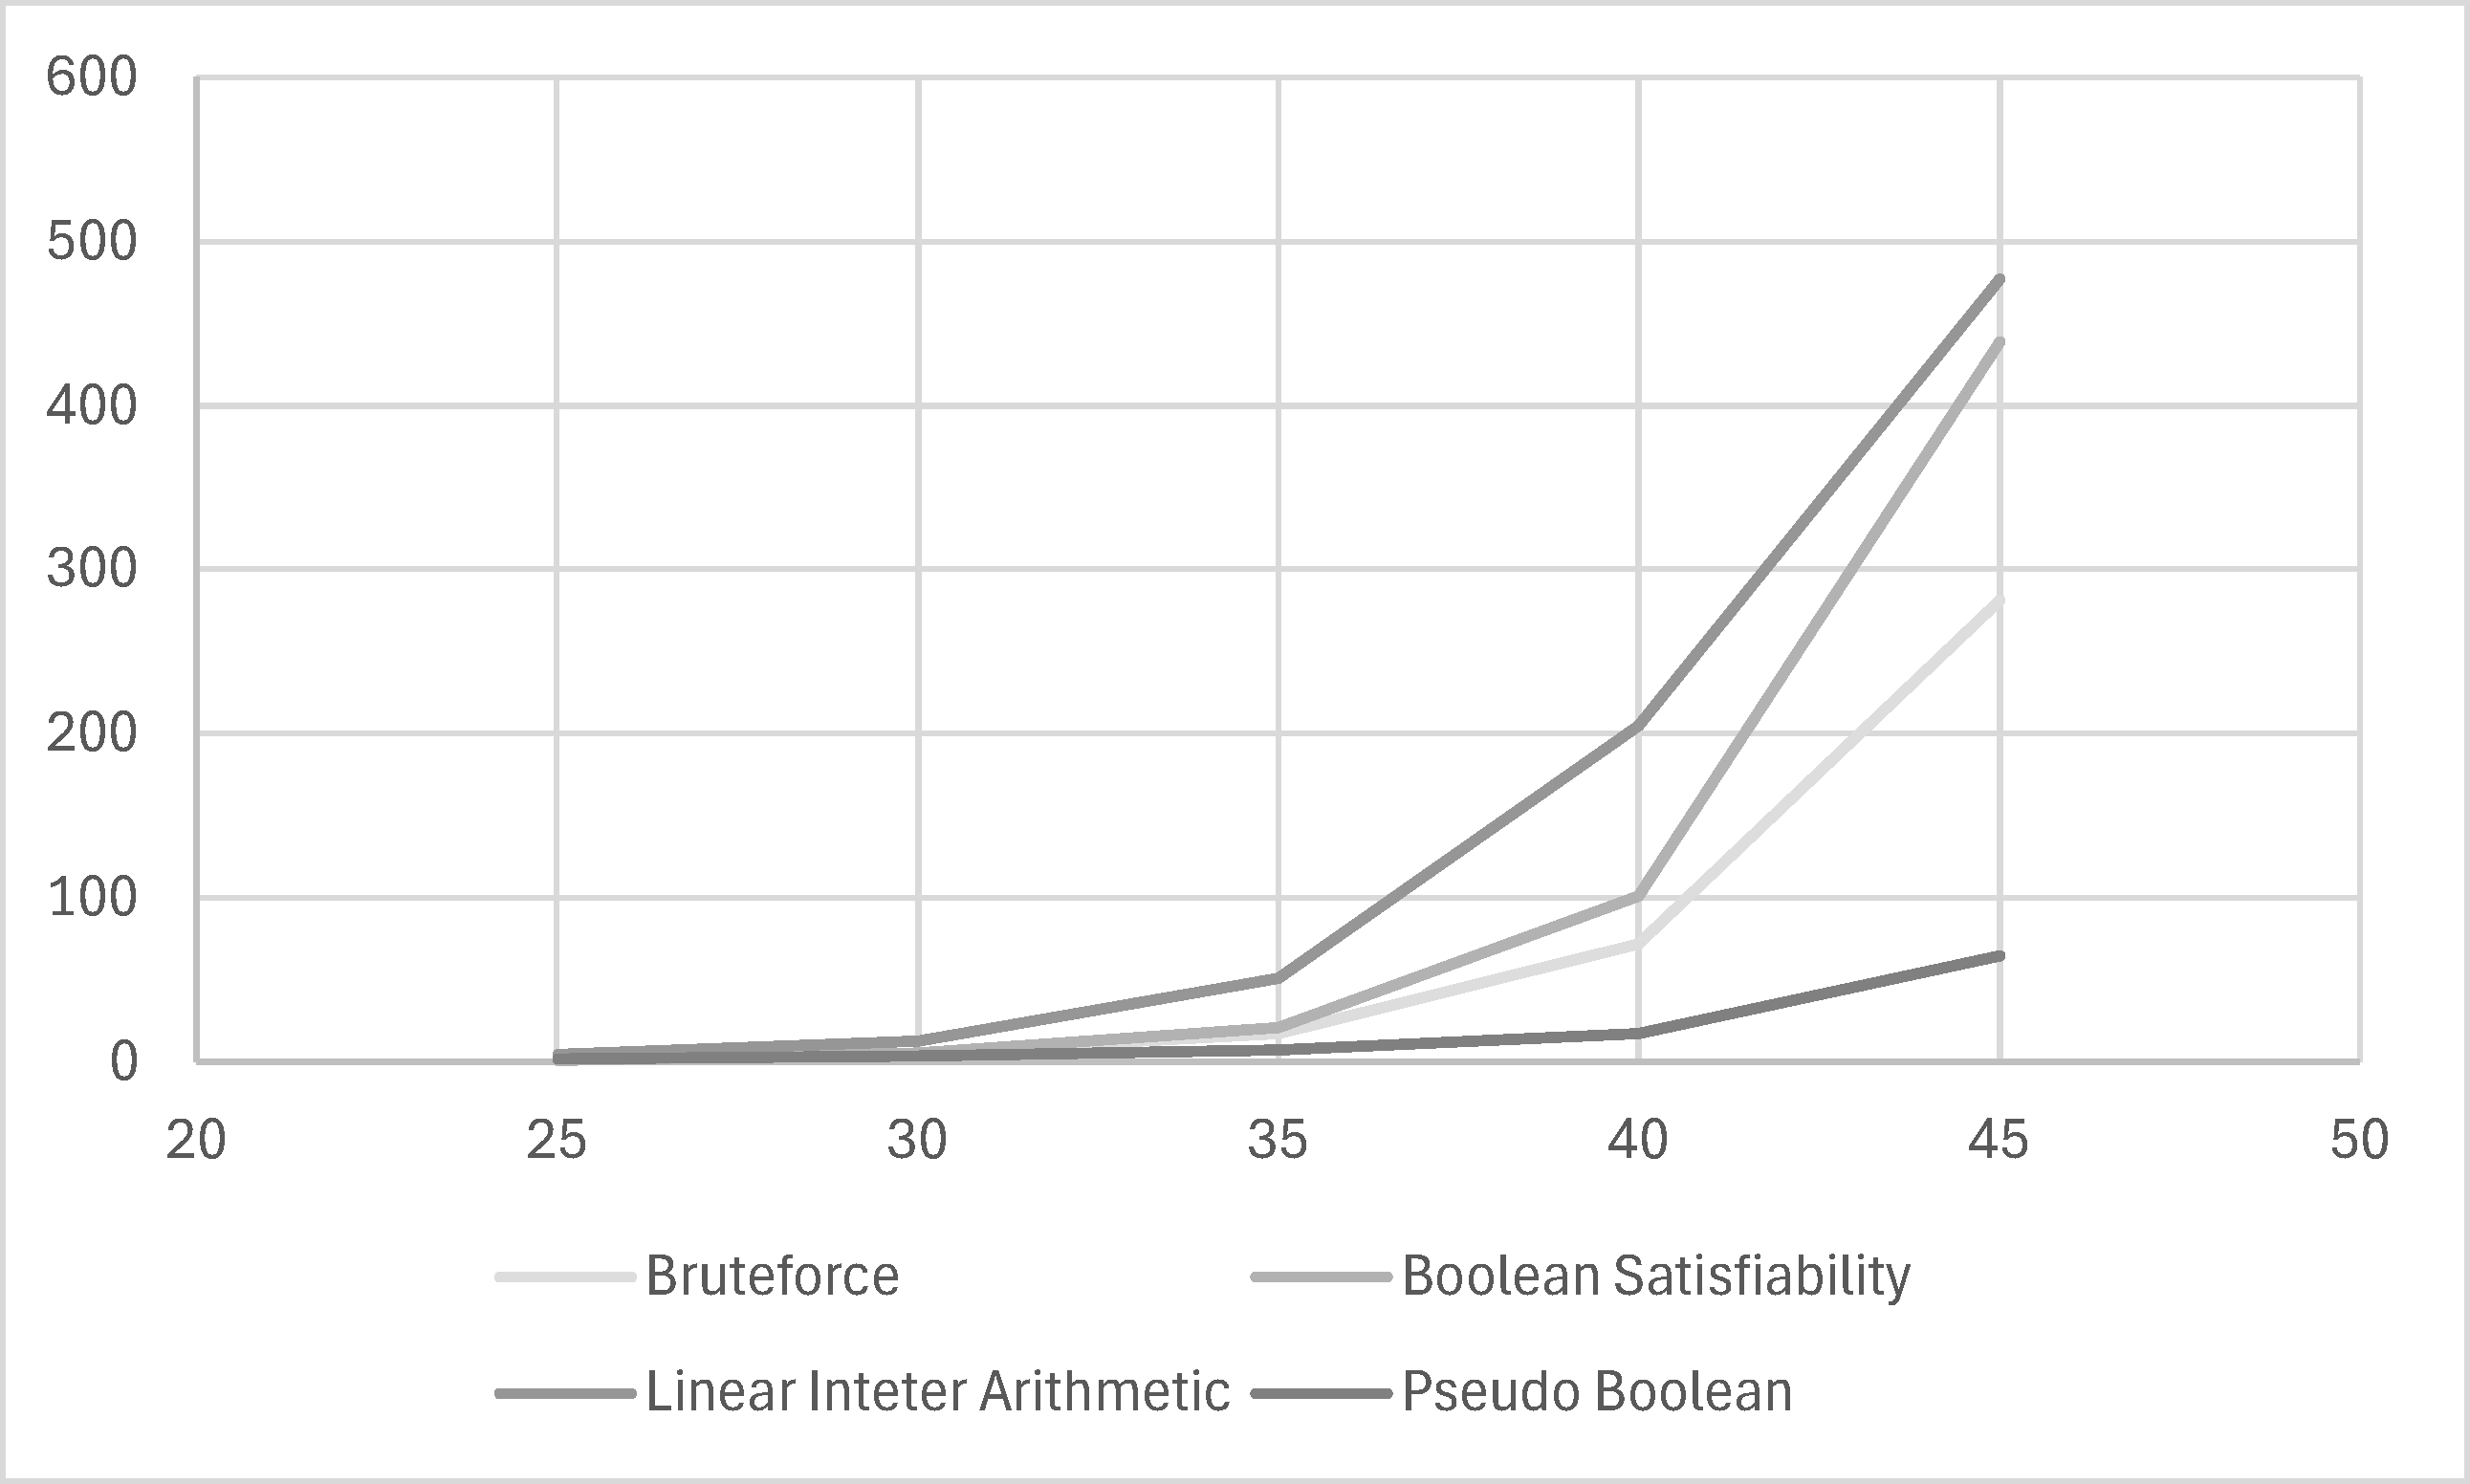
\includegraphics[width=\linewidth]{img/trend-md-large.pdf}
	\captionof{figure}{\centering Tren Waktu Eksekusi Dimensi Metrik Graf Besar}
	\label{fig:trend-md-large}
\end{minipage}


	\vspace{2em}

	\begin{minipage}[\minipagealign]{\minipagewidth}
	\centering
	\captionof{table}{\centering Rata-Rata Waktu Eksekusi Dimensi Metrik Sisi Graf Besar (Detik)}
	\resizetofit{
		\begin{tabular}{|c|c|r|r|r|r|}
			\hline \begin{tabular}[c]{@{}c@{}}Dimensi\\ Metrik Sisi\end{tabular} & \begin{tabular}[c]{@{}c@{}}Banyak\\ Simpul\end{tabular} & \multicolumn{1}{c|}{\foreign{Brute-force}} & \multicolumn{1}{c|}{\begin{tabular}[c]{@{}c@{}}\foreign{Boolean}\\ \foreign{Satisfiability}\end{tabular}} & \multicolumn{1}{c|}{\begin{tabular}[c]{@{}c@{}}\foreign{Linear Integer}\\ \foreign{Arithmetic}\end{tabular}} & \multicolumn{1}{c|}{\begin{tabular}[c]{@{}c@{}}\foreign{Pseudo}\\ \foreign{Boolean}\end{tabular}} \\ \hline 3 & 10 & .011334 & .026933 & .109807 & .041412 \\ \hline 4 & 15 & .249981 & .162525 & .543050 & .343242 \\ \hline 5 & 20 & 6.572275 & 1.022019 & 3.285489 & 2.136249 \\ \hline 5 & 25 & 236.021321 & 5.733961 & 19.858158 & 10.403642 \\ \hline 6 & 30 & & 66.906106 & 203.095024 & 47.012734 \\ \hline 6 & 35 & & 324.791564 & & 291.849713 \\ \hline 6 & 40 & & & & 500.657666 \\ \hline 6 & 45 & & & & \\ \hline 7 & 50 & & & & \\ \hline
		\end{tabular}
	}
\end{minipage}

	\hspace{2em}
	\begin{minipage}[\minipagealign]{\minipagewidth}
	\centering
	\begin{minipage}{0.427\linewidth}
		\centering
		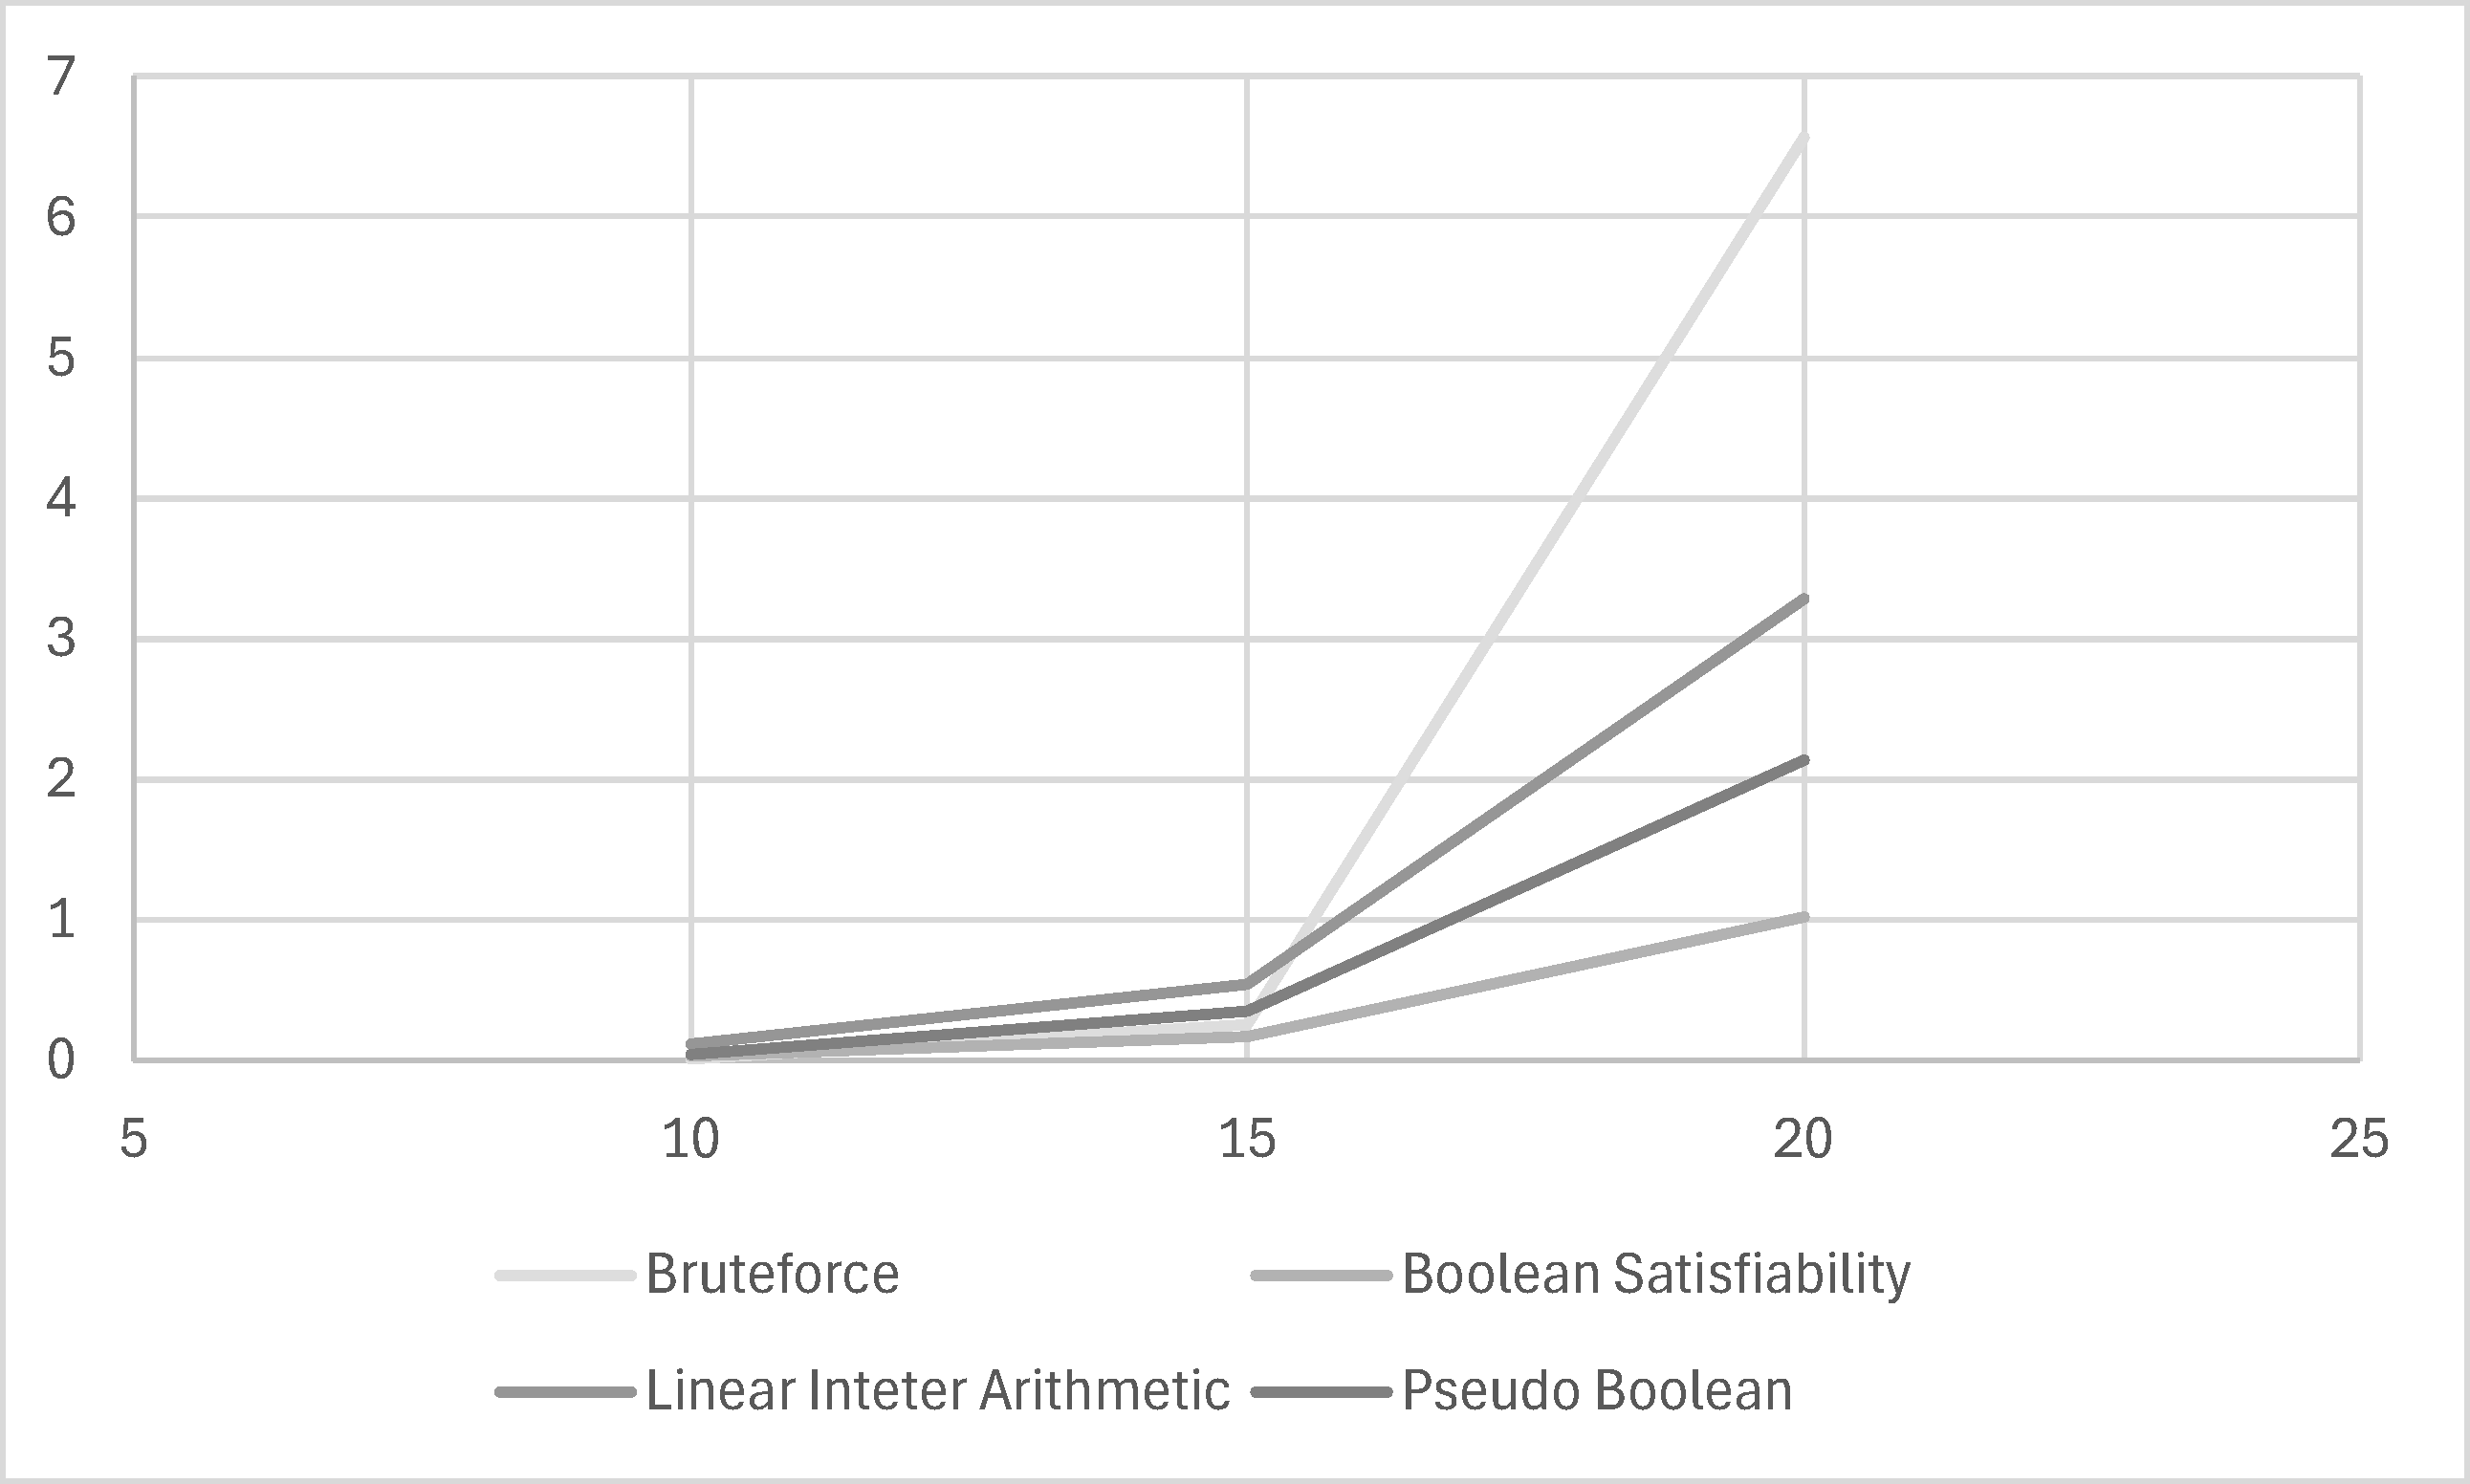
\includegraphics[width=\linewidth]{img/trend-emd-large-1.pdf}
		\par\small (a)
	\end{minipage}
	\hfill
	\begin{minipage}{0.549\linewidth}
		\centering
		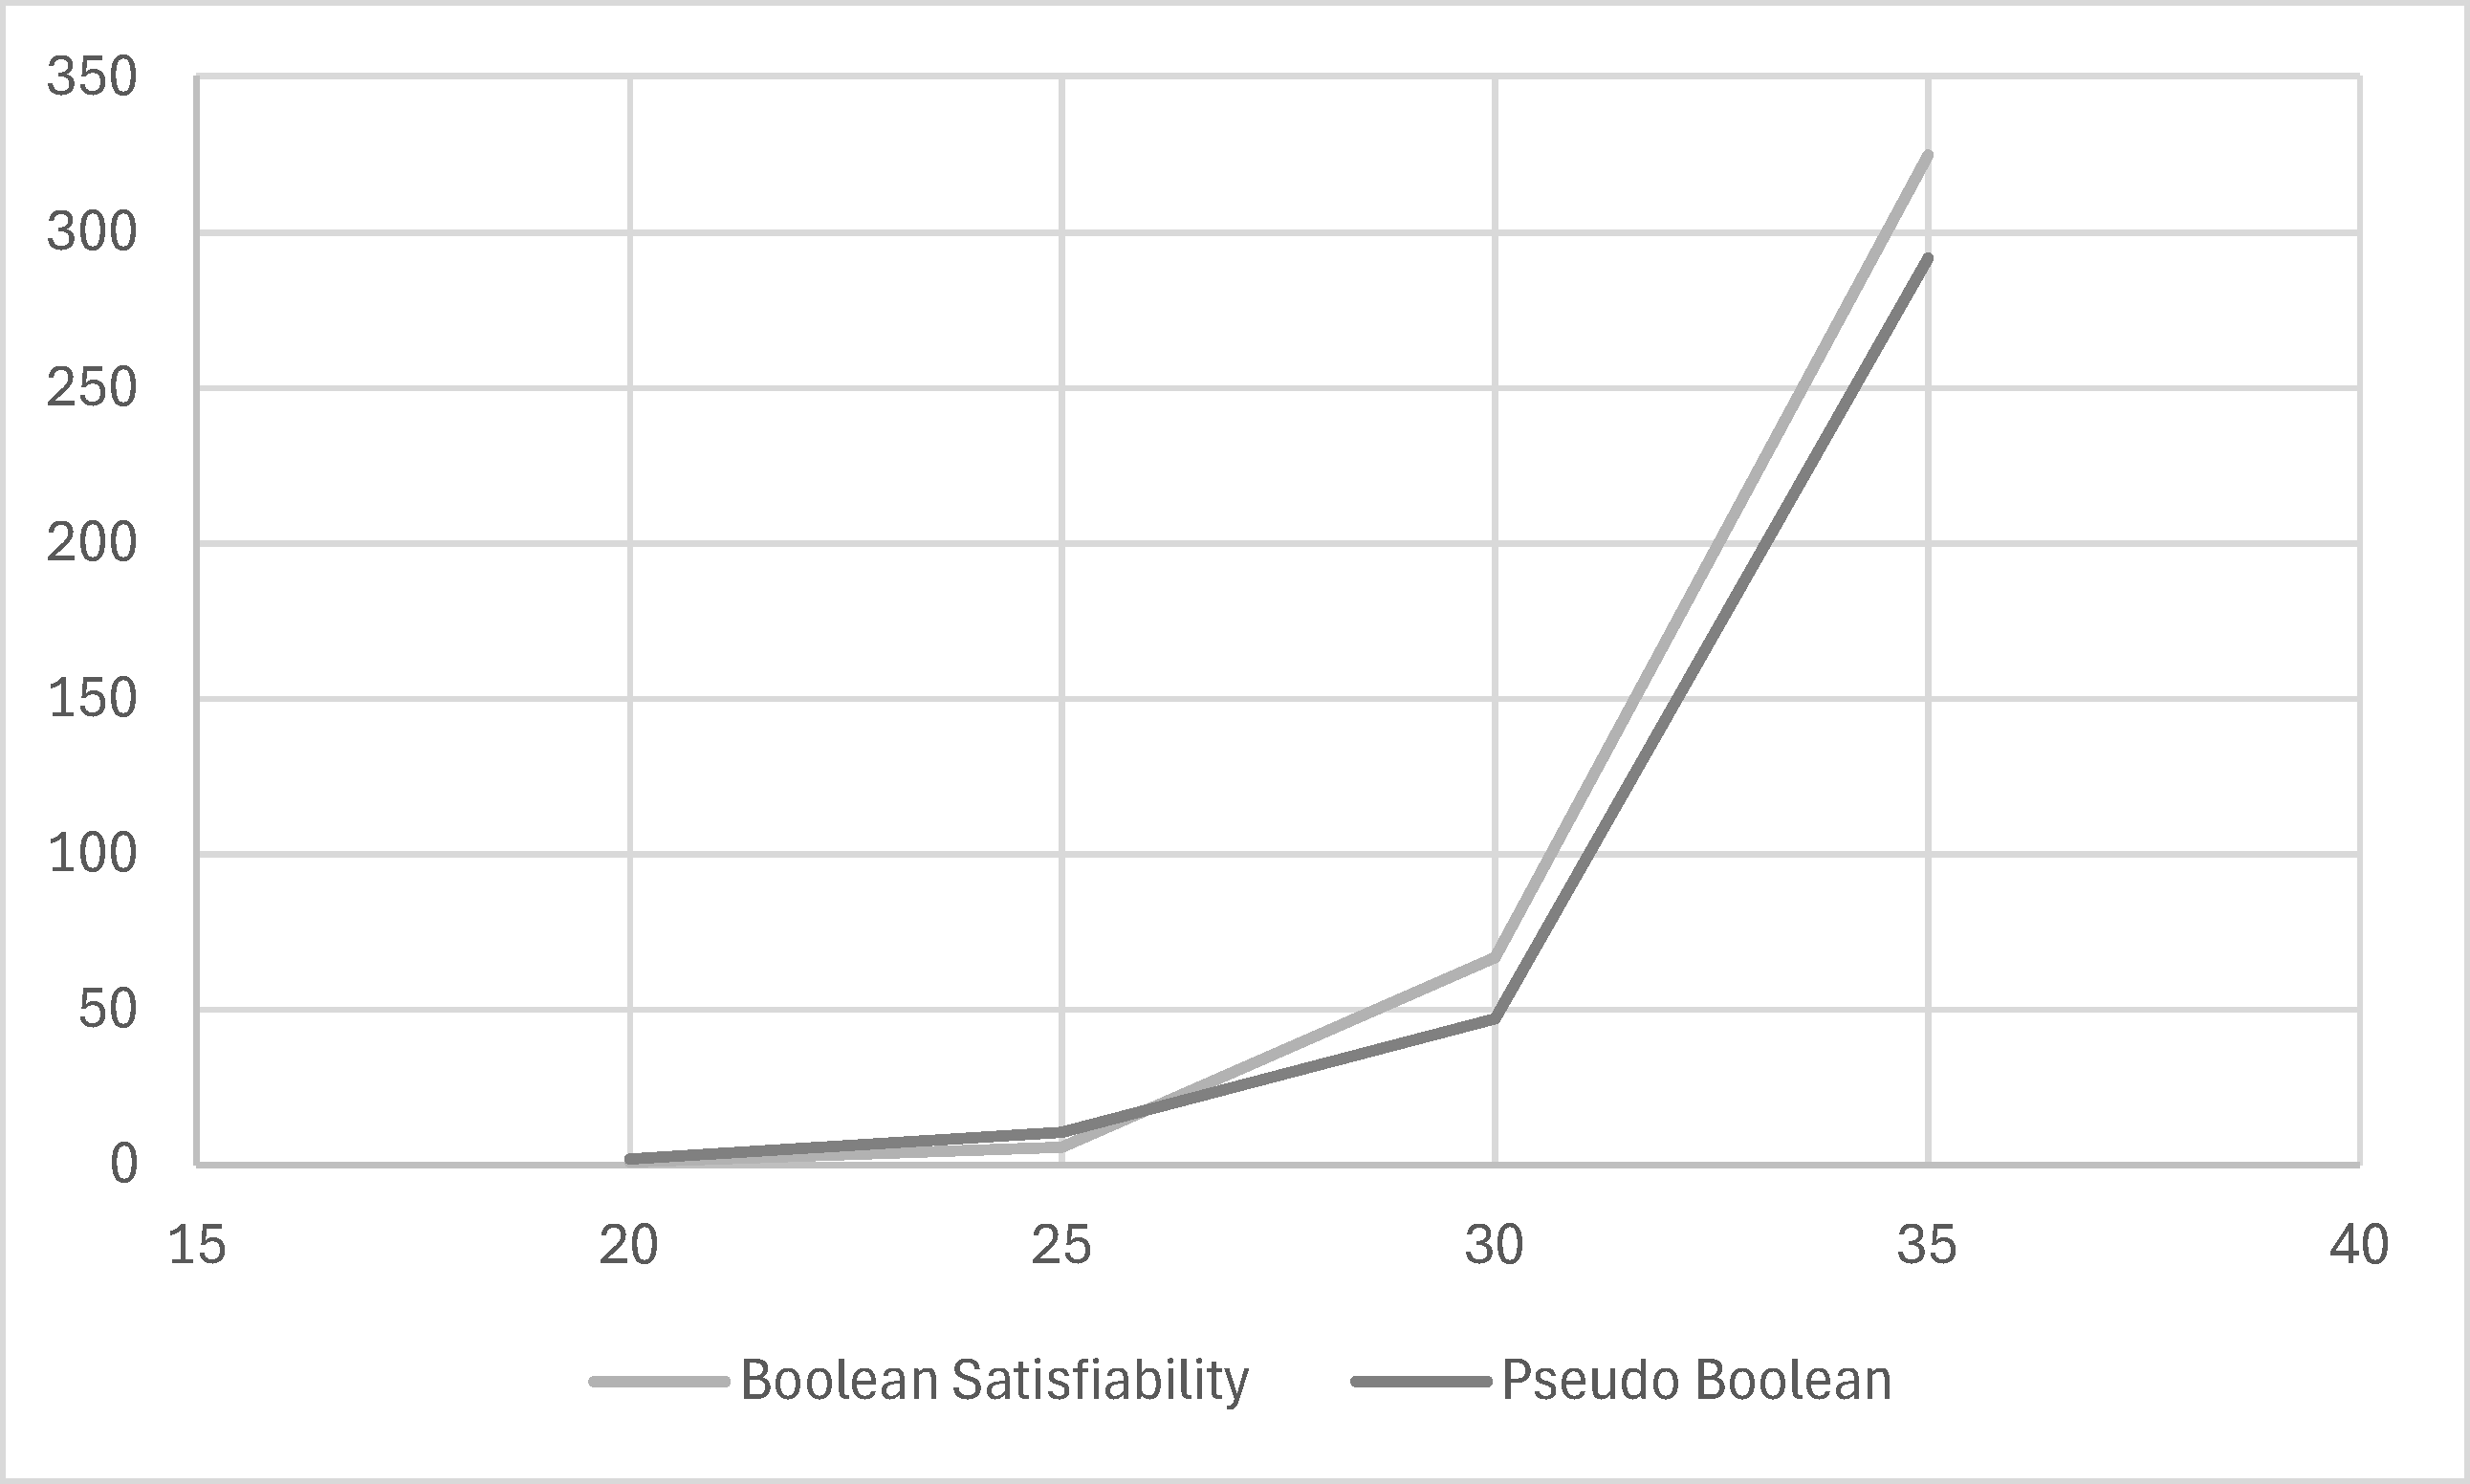
\includegraphics[width=\linewidth]{img/trend-emd-large-2.pdf}
		\par\small (b)
	\end{minipage}
	\captionof{figure}{\centering Tren Waktu Eksekusi Dimensi Metrik Sisi Graf Besar}
	\label{fig:trend-emd-large}
\end{minipage}


	\vfill \vfill \vfill
\end{center}
\end{landscape}

\section{Pembahasan Keseluruhan Hasil Eksekusi}
\label{sec:discussion-combined}

Ketiga, dibahas hasil eksekusi secara keseluruhan untuk memberikan gambaran lebih jelas mengenai waktu eksekusi masing-masing algoritma. Dengan menggabungkan \autoref{tab:mean-md-small} dan \autoref{tab:mean-md-large} dan mengilustrasikannya sebagai satu grafik tren pada \autoref{fig:trend-md-combined}, didapatkan gambaran yang lebih lengkap mengenai waktu eksekusi untuk graf kecil dan besar. Menggunakan cara yang sama, \autoref{tab:mean-emd-small} dan \autoref{tab:mean-emd-large} digabungkan dan diilustrasikan dalam satu grafik tren pada \autoref{fig:trend-emd-combined}; grafik ini dipecah menjadi (a) dan (b) untuk alasan yang sama seperti pada \autoref{fig:trend-emd-large}. Seluruh ilustrasi gabungan ini menggunakan skala logaritma pada sumbu vertikal karena naiknya waktu eksekusi yang cenderung bersifat kombinatorial, sesuai dengan pembahasan pada \autoref{subsec:bf}.

Untuk penentuan dimensi metrik, terlihat pada \autoref{fig:trend-md-combined} bahwa \autoref{alg:brute-force} unggul dari graf bersimpul 2 hingga 20. Selanjutnya, \autoref{alg:boolean-satisfiability} unggul dari graf bersimpul 25 hingga 30. Untuk graf bersimpul 35 atau lebih, \autoref{alg:pseudo-boolean} menjadi yang paling unggul. Sementara itu, \autoref{alg:linear-integer-arithmetic} selalu memiliki waktu eksekusi paling lambat untuk semua graf.

Kemudian, untuk penentuan dimensi metrik sisi, sebagaimana terlihat pada \autoref{fig:trend-emd-combined}, \autoref{alg:brute-force} unggul dari graf bersimpul 2 hingga 10. Mirip seperti sebelumnya, \autoref{alg:boolean-satisfiability} unggul dari graf bersimpul 15 hingga 25. Akhirnya, \autoref{alg:pseudo-boolean} adalah yang paling unggul untuk graf bersimpul 30 atau lebih. Sekali lagi, \autoref{alg:linear-integer-arithmetic} merupakan algoritma dengan waktu eksekusi paling lambat.

Dengan demikian, secara keseluruhan, hasil ini menunjukkan bahwa \autoref{alg:brute-force} lebih unggul pada graf kecil, sedangkan \autoref{alg:pseudo-boolean} lebih unggul pada graf besar. Lalu, \autoref{alg:boolean-satisfiability} merupakan \foreign{trade-off} yang dapat diambil dalam implementasi umum untuk transisi dari komputasi pada graf kecil ke graf besar.

\begin{center}
	\renewcommand{\minipagewidth}{0.9\linewidth}

	\begin{figure}
	\centering
	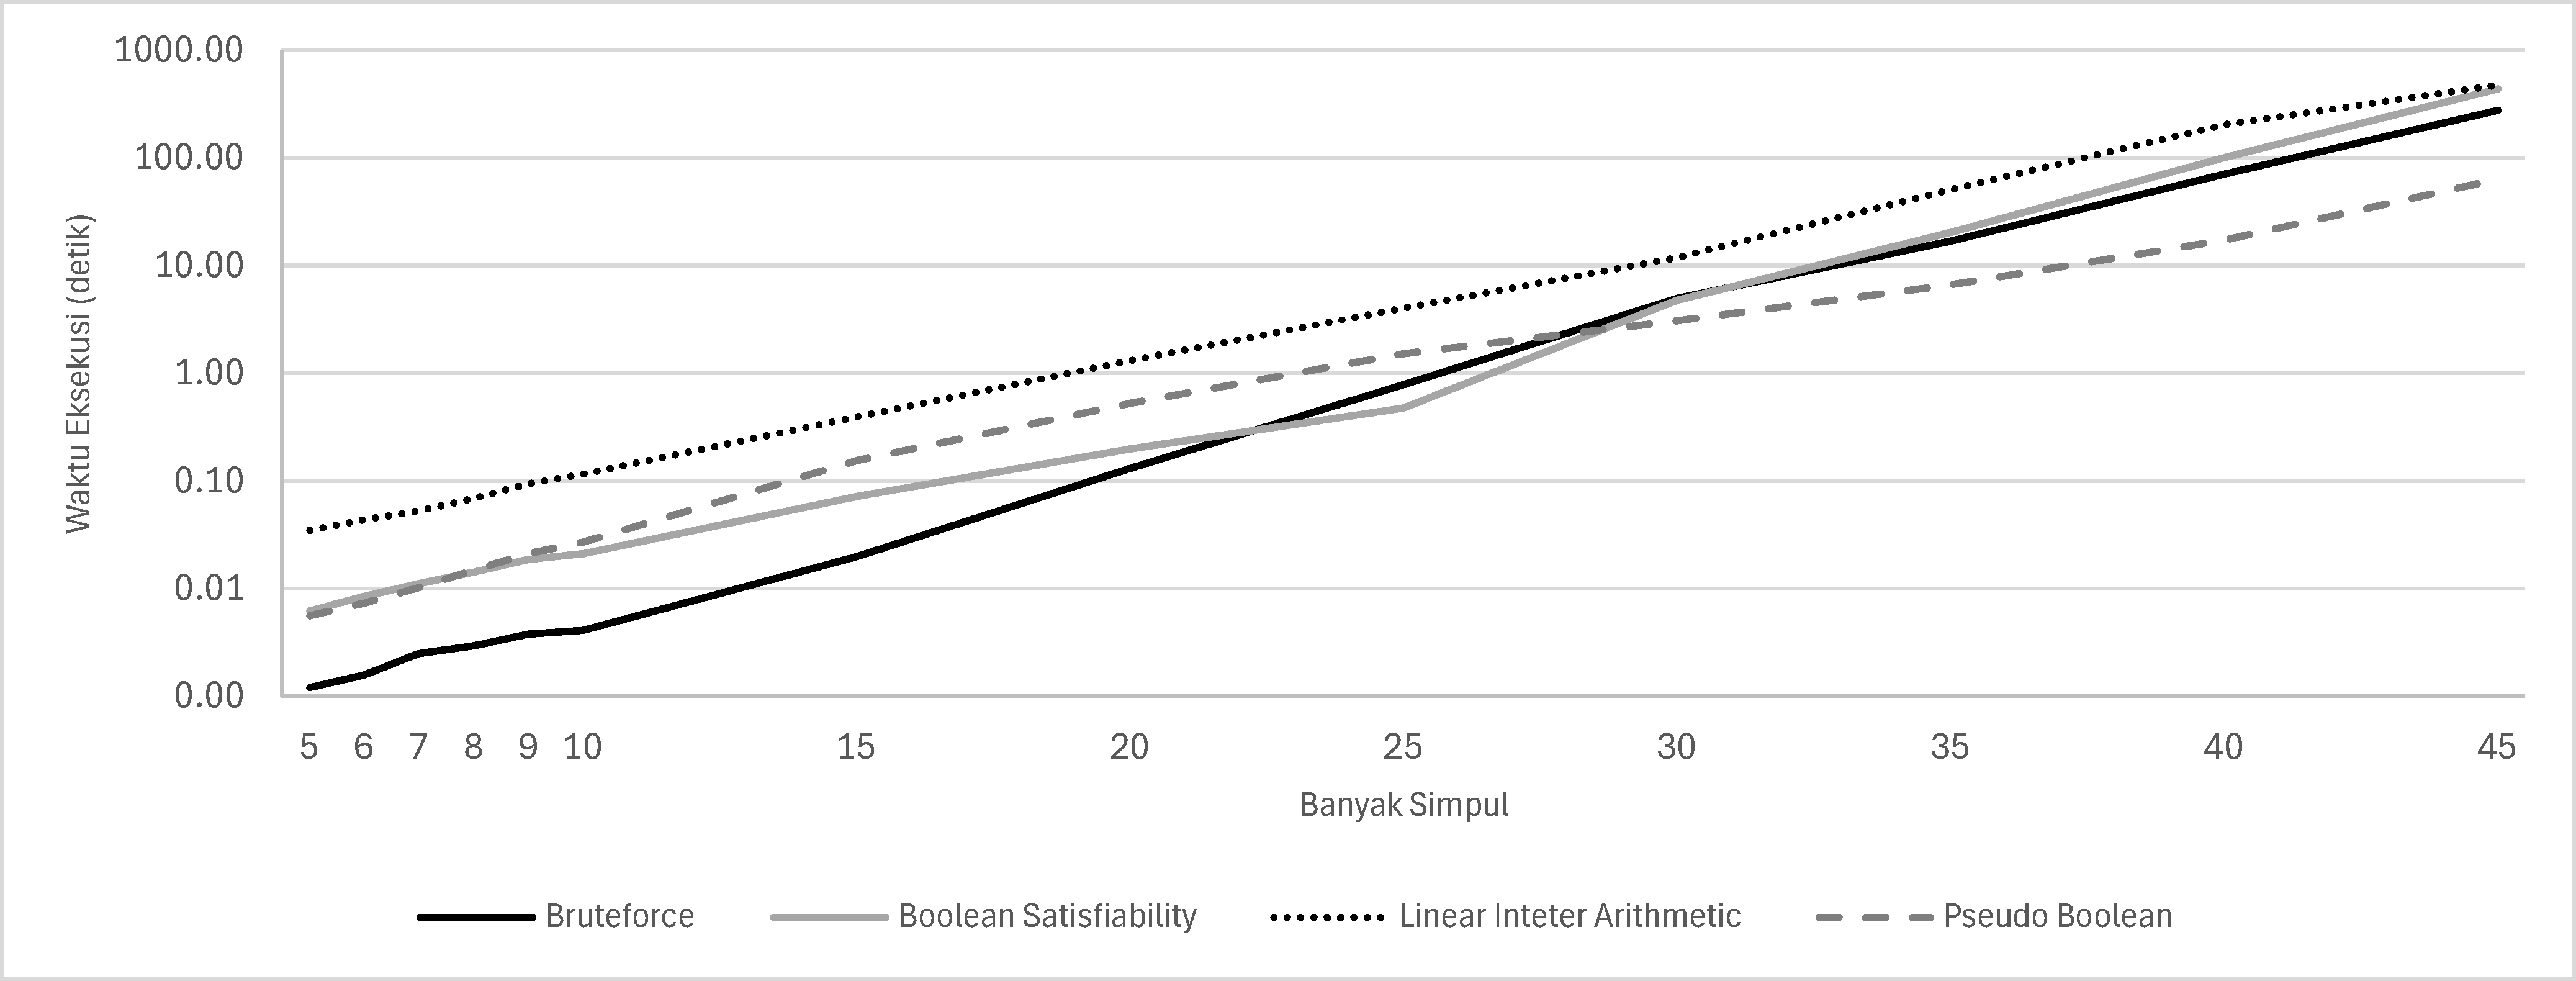
\includegraphics[width=.65\linewidth]{img/trend-md-combined.pdf}
	\caption{Trend Dimensi Metrik}
\end{figure}


	\vspace{0.5em}

	\begin{minipage}[\minipagealign]{\minipagewidth}
	\centering
	\begin{minipage}{0.686\linewidth}
		\centering
		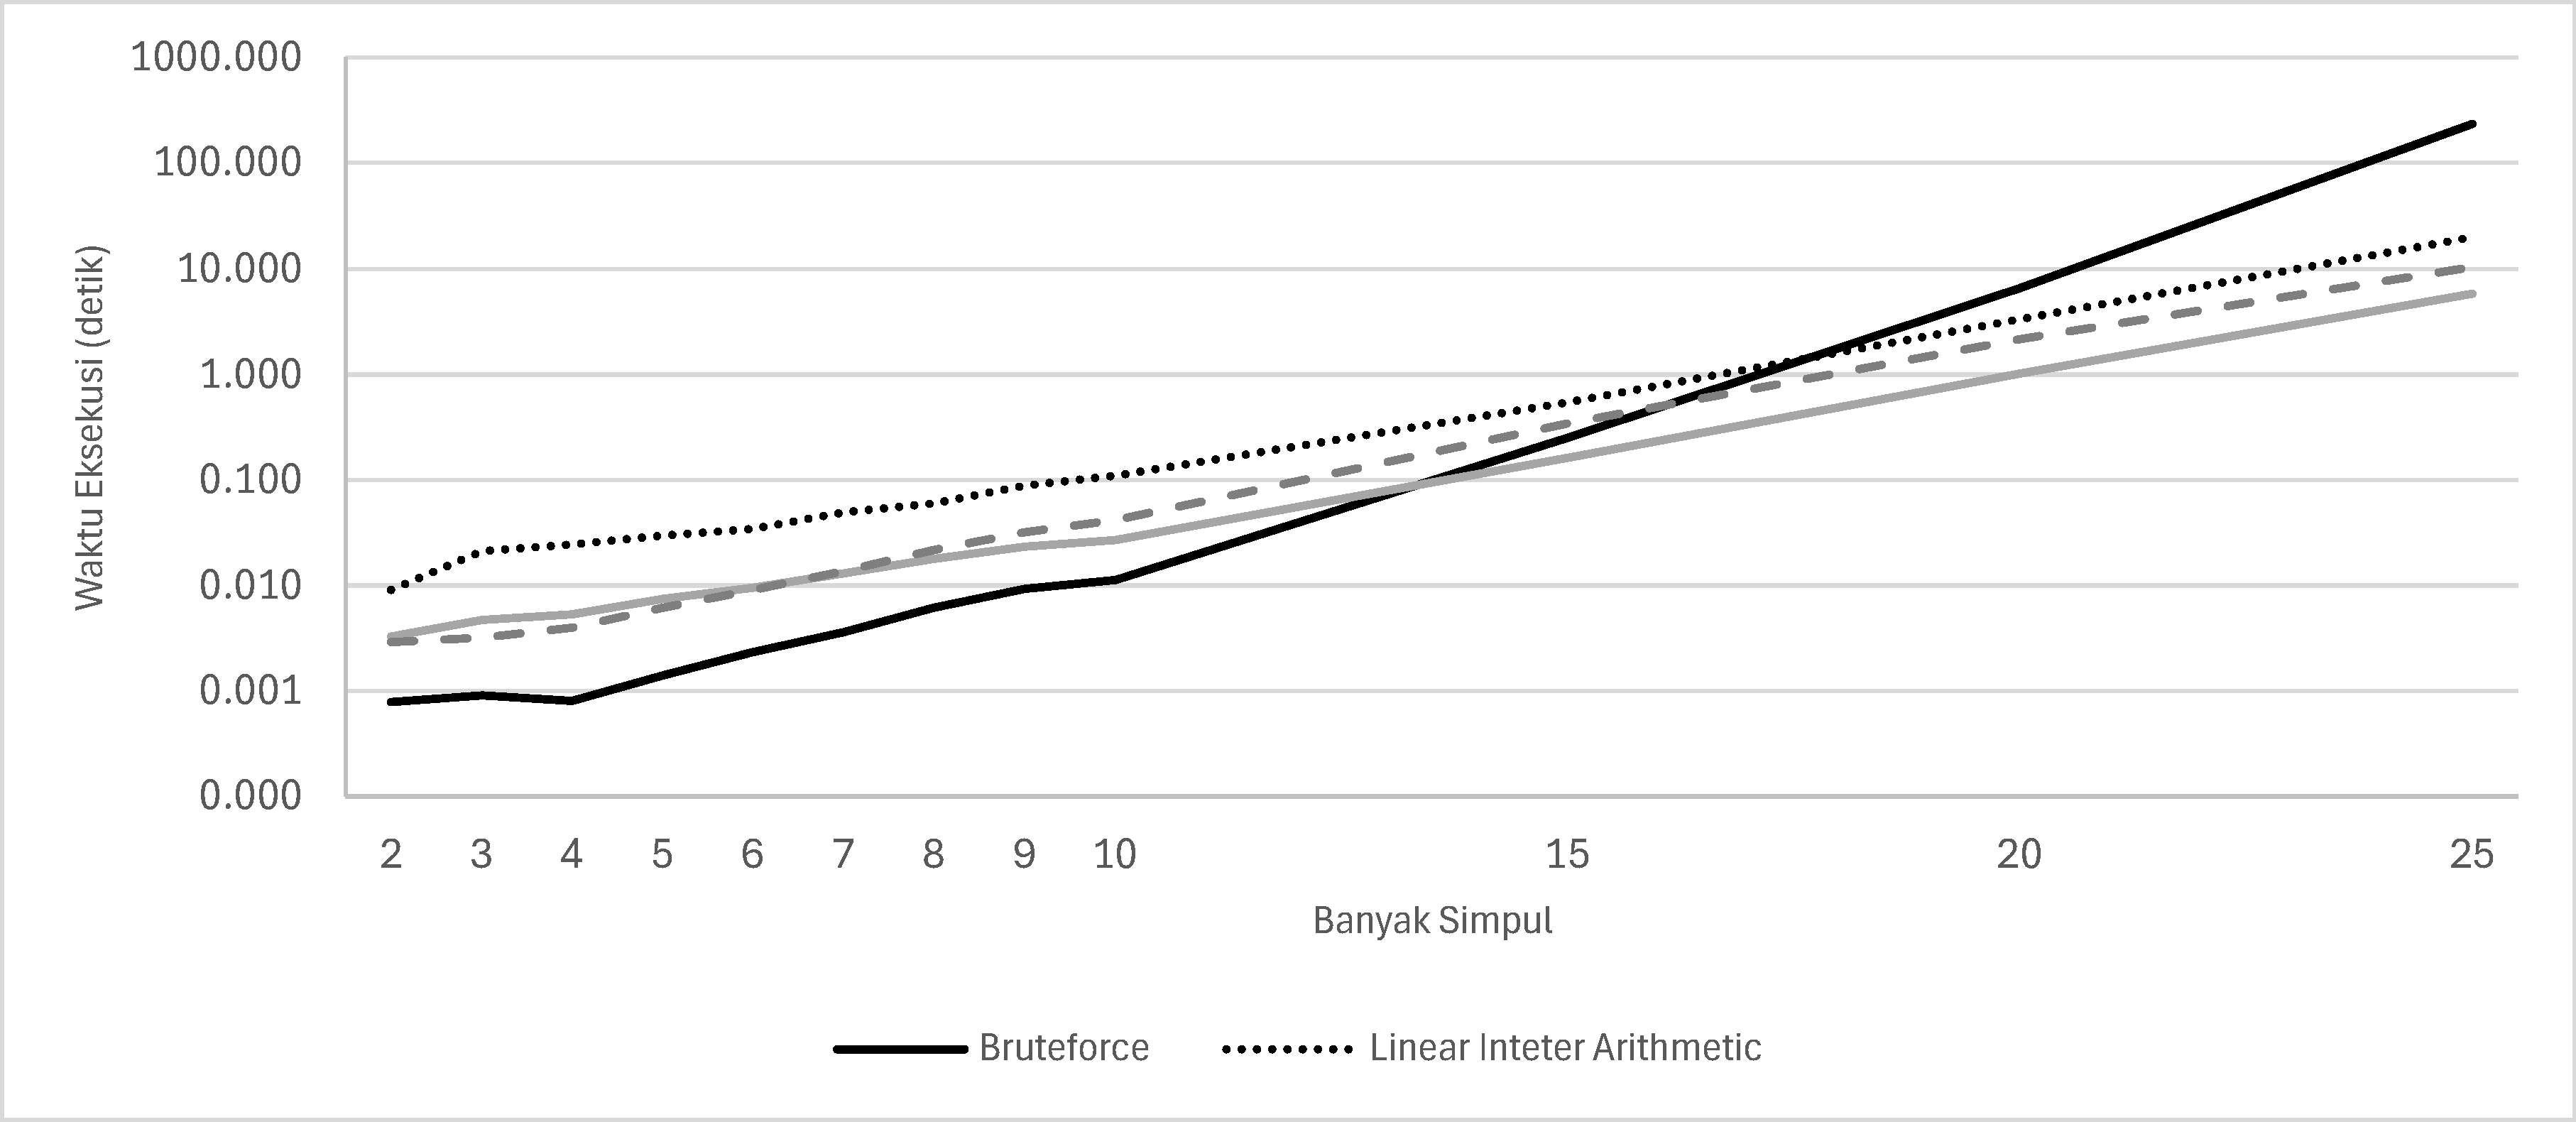
\includegraphics[width=\linewidth]{img/trend-emd-combined-1.pdf}
		\par\small (a)
	\end{minipage}
	\begin{minipage}{0.294\linewidth}
		\centering
		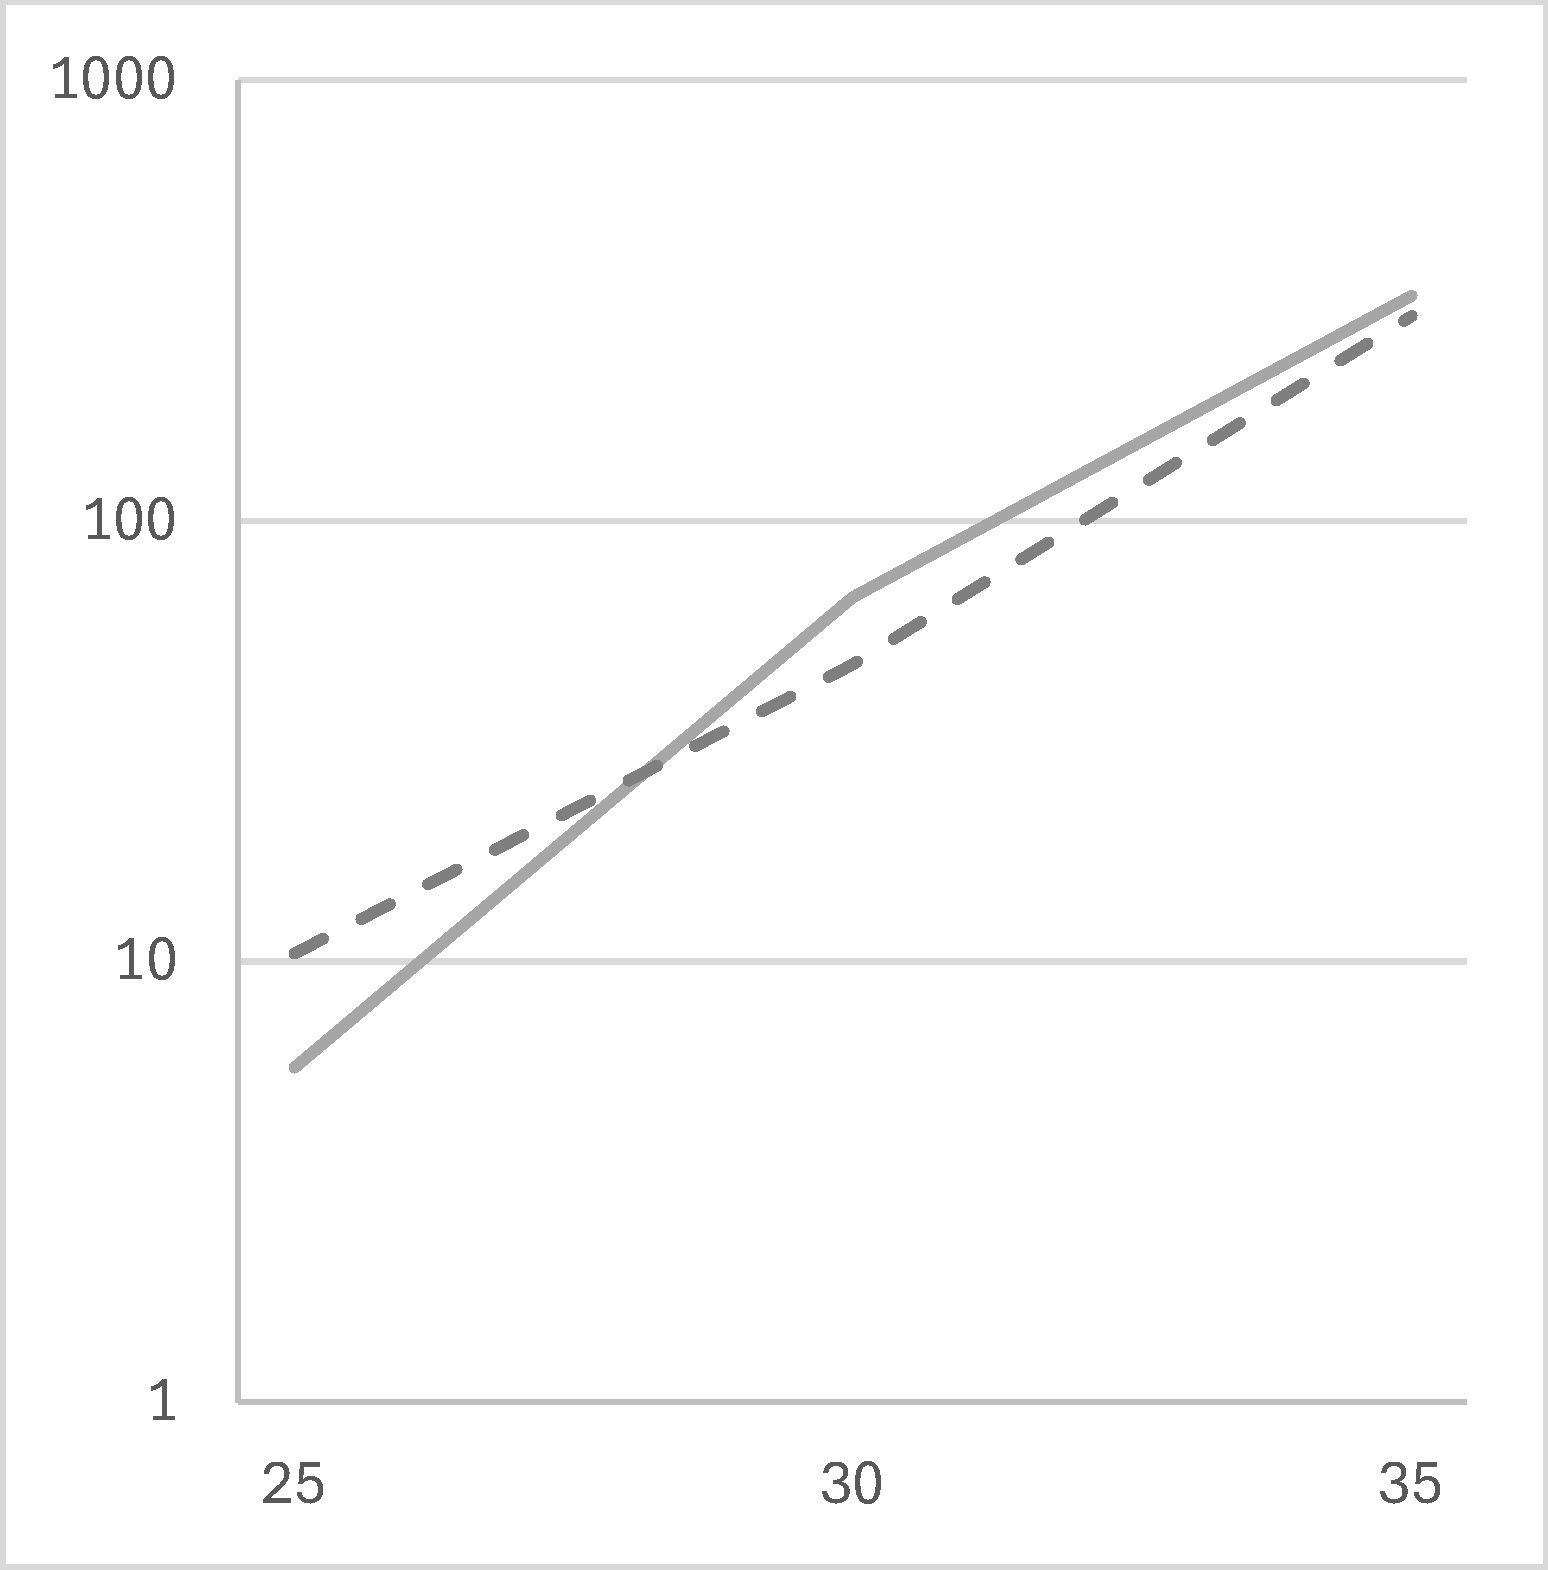
\includegraphics[width=\linewidth]{img/trend-emd-combined-2.pdf}
		\par\small (b)
	\end{minipage}
	\captionof{figure}{\centering Tren Waktu Eksekusi Dimensi Metrik Sisi}
	\label{fig:trend-emd-combined}
\end{minipage}

\end{center}


	\cleardoublepage

	\chapter{Kesimpulan dan Saran}

\section{Kesimpulan}

Tugas akhir ini bertujuan untuk mempelajari permasalahan penentuan invarian graf berupa dimensi metrik dan dimensi metrik sisi dengan memanfaatkan pendekatan berbasis \foreign{Satisfiability Modulo Theories} (SMT). Fokus tugas akhir ini meliputi hal-hal dari formulasi permasalahan ke dalam bentuk SMT, pengimplementasian formulasi tersebut, hingga evaluasi efektivitas pendekatan yang diusulkan. Berdasarkan hasil yang telah diperoleh, dapat disimpulkan bahwa:

\begin{enumerate}
	\item Permasalahan dimensi metrik dan dimensi metrik sisi dapat direpresentasikan secara sistematis ke dalam bentuk formula SMT, sebagaimana telah didemonstrasikan oleh \autoref{alg:boolean-satisfiability}, \autoref{alg:linear-integer-arithmetic}, dan \autoref{alg:pseudo-boolean}.

	\item Pendekatan SMT dapat digunakan secara praktikal untuk menentukan dimensi metrik maupun dimensi metrik sisi suatu graf. Terlihat dari hasil pada \autoref{sec:implementation} dan tabel-tabel frekuensi pada \autoref{sec:discussion-small} dan \autoref{sec:discussion-large} bahwa strategi tersebut dapat menghasilkan kedua invarian ini dengan benar.

	\item Efektivitas penggunaan SMT dalam menyelesaikan permasalahan dimensi metrik dan dimensi metrik sisi bergantung pada ukuran graf dan sumber daya komputasi yang tersedia, serta pemilihan teori yang digunakan -- seperti yang telah dikaji pada \autoref{sec:discussion-combined}.
\end{enumerate}

Kesimpulan yang diperoleh dalam tugas akhir ini berlaku dalam batasan-batasan yang telah ditetapkan. Yaitu pemilihan graf yang sederhana, tak berarah, terhubung, dan tak berbobot; banyaknya simpul pada graf yang dibatasi sesuai dengan perencanaan pada \autoref{sec:data}; membatasi waktu eksekusi; serta melakukan eksekusi implementasi menggunakan \foreign{CPU} yang telah dispesifikasikan. Semua hal ini dielaborasikan lebih detail pada \autoref{sec:implementation}. Kebenaran hasil penentuan dimensi metrik atau dimensi metrik sisi menggunakan SMT juga dibantu validasi melalui metode \foreign{brute-force} selama \autoref{alg:brute-force} masih mampu melakukan komputasinya dengan batasan-batasan ini.

Dengan demikian, secara keseluruhan, hasil tugas akhir ini menunjukkan bahwa memetakan suatu perumusan ke dalam SMT merupakan alternatif pendekatan yang layaknya cukup tajam untuk secara sistematis menghadapi permasalahan graf yang relatif rumit, seperti penentuan dimensi metrik dan dimensi metrik sisi.

Diharapkan pekerjaan yang telah dicapai dalam tugas akhir ini berhasil membawa beberapa manfaat. Seperti langkah-langkah analisis yang dilakukan dalam usaha memformulasi permasalahan graf ke dalam SMT diharapkan berkontribusi memberi wawasan baru dalam pengembangan pembelajaran teori graf secara komputasional. Atau cara pemetaan rumusan penentuan dimensi metrik dan dimensi metrik sisi spesifik pada tugas akhir ini yang mungkin menjadi dasar awal untuk pengembangan lebih lanjut. Maupun dokumentasi, implementasi, dan hasil yang diperoleh dapat menjadi referensi bagi tugas akhir atau penelitian selanjutnya dalam teori graf serta bidang ilmu komputer.

\section{Saran}

Banyak aspek dari tugas akhir ini yang masih dapat dikembangkan lebih lanjut. Bagian ini menyajikan beberapa saran sebagai bahan pertimbangan untuk area-area yang dapat dipelajari lebih lanjut. Diskusi saran di sini mencakup aspek lingkup eksperimen, implementasi algoritma, desain algoritma, eksekusi eksperimen, variasi graf, alternatif teori, serta eksplorasi aplikasi.

Secara lingkup eksperimen, batasan-batasan sebagaimana pada \autoref{sec:implementation} dipilih atas pertimbangan praktikalitas pengerjaan dengan waktu dan sumber daya yang tersedia dalam penyusunan tugas akhir ini. Namun, dengan telah selesainya perancangan teori yang mendasari formulasi algoritma-algoritma sebagaimana pada \autoref{sec:alg}, skema eksekusi eksperimen dapat dikembangkan lebih lanjut. Misalnya, evaluasi dapat dilakukan pada graf berukuran lebih besar, mengingat evaluasi pada tugas akhir ini dibatasi hingga 50 simpul. Dengan demikian, batasan waktu eksekusi per iterasi dalam tugas akhir ini yang ditetapkan selama 5 menit dapat diperpanjang untuk mendukung evaluasi graf lebih besar, seiring meningkatnya waktu eksekusi yang cenderung bersifat kombinatorial. Perlu diperhatikan pula strategi implementasi konstruksi \foreign{distance similarity matrix} agar kompleksitas waktu dan ruang memori dapat mengatasi graf dengan lebih banyak simpul. Selain itu, interval kenaikan banyak simpul untuk graf besar dapat diperkecil. Dalam tugas akhir ini, interval yang digunakan relatif besar, yaitu 5 simpul. Dengan interval kenaikan simpul lebih kecil, tren seperti pada \autoref{sec:discussion-small}, \autoref{sec:discussion-large}, dan \autoref{sec:discussion-combined} dapat diperoleh dengan resolusi lebih tinggi, sehingga analisis yang dilakukan dapat menjadi lebih spesifik. Selanjutnya, karena data analisis untuk graf besar pada dasarnya merupakan sampel dari seluruh kemungkinan graf yang ada, maka dapat diambil lebih banyak data. Dalam tugas akhir ini diambil 50 graf sembarang untuk setiap graf bersimpul \(n\); dengan memperbanyak graf yang dievaluasi, karakteristik tabel frekuensi untuk graf besar serta hasil perhitungan rata-rata waktu eksekusi diharapkan dapat menggambarkan variasi antar algoritma yang lebih kaya.

Secara implementasi algoritma, dapat dilakukan modifikasi cara penerapan batasan waktu eksekusi. Pada tugas akhir ini, batas waktu diberikan pada setiap iterasi kardinalitasnya. Hal ini dapat diubah menjadi batasan waktu secara eksekusi total algoritma, yaitu dari awal hingga akhir ditemukannya dimensi metrik ataupun dimensi metrik sisi.

Secara desain algoritma, terdapat tiga arah pengembangan yang dapat dilakukan. Yang paling sederhana adalah aspek perbandingan algoritma terhadap metode \foreign{brute-force}. Dalam tugas akhir ini, desain algoritma \foreign{brute-force} menggunakan landasan teori yang sama dengan algoritma berbasis SMT. Oleh karena itu, artinya metode ini tidak sepenuhnya murni \foreign{brute-force}. Analisis dapat dikembangkan dengan mendesain algoritma \foreign{brute-force} yang lebih \foreign{naive}, dan melihat apakah perbandingan evaluasi terhadap \foreign{brute-force} baru ini menghasilkan kesimpulan yang sama seperti yang ditarik pada \autoref{sec:discussion-small} dan \autoref{sec:discussion-large}. Berikutnya, aspek yang lebih menarik adalah mencoba teori lain dalam SMT, karena tugas akhir ini baru mengeksplorasi pemetaan \foreign{constraint} ke dalam \foreign{boolean satisfiability}, \foreign{linear integer arithmetic}, dan \foreign{pseudo boolean}. Mungkin terdapat teori SMT dengan \foreign{construct} yang lebih tinggi ataupun lebih rendah yang dapat menghasilkan waktu eksekusi lebih cepat, baik untuk graf kecil maupun graf besar. Akhirnya, aspek yang paling menantang untuk dikembangkan adalah mempelajari cara kerja \foreign{conflict driven learning} yang fundamental dalam SMT, dan memformulasi pemetaan yang dapat mengeksploitasi mekanisme ini dengan lebih efektif.

Secara eksekusi eksperimen, terdapat dua pendekatan yang dapat dicoba. Pertama adalah menggunakan \foreign{solver} SMT selain Z3. Kedua adalah menggunakan \foreign{solver} yang memiliki kemampuan \foreign{parallelism}, sehingga dapat memanfaatkan \foreign{multi-core} untuk eksekusi satu individu graf, tanpa mengubah kode implementasi sama sekali. Hasil yang diperoleh dari kedua pendekatan ini kemudian dapat dibandingkan dengan hasil eksekusi klasik menggunakan Z3.

Secara variasi graf, terdapat banyak variasi yang dapat dilakukan. Beberapa contohnya dijelaskan berikut ini. Contoh yang paling jelas adalah dimensi metrik itu sendiri. Tugas akhir ini hanya mengkaji dimensi metrik pada bentuk klasiknya dan dimensi metrik sisi. Beberapa contoh variasi dimensi metrik yang dapat dicoba antara lain adalah \foreign{local metric dimension}, \foreign{mixed metric dimension}, \foreign{k-metric dimension}, \foreign{fault tolerant metric dimension}, \foreign{strong metric dimension}, dan variasi lainnya. Hal lain yang dapat diubah adalah asumsi dalam graf yang digunakan untuk menentukan dimensi metrik itu sendiri. Contohnya, dapat dicoba graf berbobot, atau graf berarah, atau graf tak sederhana, dan sebagainya.

Secara alternatif teori, yang dimaksud adalah pengembangan dari landasan teori fundamental yang telah dikerjakan oleh tugas akhir ini untuk desain setiap algoritmanya, yaitu \foreign{distance similarity matrix}. Pertama, representasi matriks paling optimal ketika graf yang bersangkutan cenderung \foreign{dense}. Sehingga, teori ini dapat dieksplorasi lebih lanjut sifat-sifatnya untuk graf yang cenderung \foreign{sparse}, dan apakah mampu dimodifikasi agar lebih efisien. Kedua, dapat dipelajari lebih lanjut apakah struktur \foreign{distance similarity matrix} ramah untuk melakukan optimasi menggunakan metode \foreign{divide and conquer}, atau apakah matriks ini memiliki struktur yang cukup terkait satu sama lain sehingga menghentikan pendekatan ini. Ketiga, dapat dipelajari apakah pemetaan \foreign{distance similarity matrix} ke \foreign{constraint} dalam SMT mungkin untuk dikonstruksikan sedemikian rupa ramah terhadap paralelisasi. Keempat, eksplorasi teori-teori graf lainnya yang mungkin dapat dimanfaatkan untuk mengambil inferensi dari maupun melakukan transformasi pada \foreign{distance similarity matrix}.

Terakhir, adalah eksplorasi aplikasi. Di luar aplikasi yang telah dibahas pada \autoref{sec:application}, masih banyak lagi potensi penggunaan dimensi metrik yang dapat dieksplorasi, misalnya dalam bidang kimia. Simpul dapat dimodelkan sebagai atom dan sisi sebagai ikatan; dimensi metrik dapat digunakan untuk analisis terkait atom, seperti analisis pola struktural, sedangkan dimensi metrik sisi dapat digunakan untuk analisis terkait ikatan, seperti analisis functional group. Beberapa contoh aplikasinya antara lain adalah:

\begin{enumerate}
	\item Banyak senyawa kimia memiliki komposisi elemen yang sama tetapi struktur berbeda. Dimensi metrik dapat digunakan untuk identifikasi isomer.

	\item Banyak senyawa kimia memiliki derajat kesimetrian yang tinggi, sehingga mereka tampak sama secara lokal. Dimensi metrik sisi dapat digunakan untuk memecah kesimetrian topologi.

	\item Dalam machine learning, biasanya diperlukan data dalam bentuk vektor, sedangkan senyawa kimia biasanya direpresentasikan dalam bentuk simbolik. Dimensi metrik berpotensi berfungsi sebagai encoding yang efektif untuk merepresentasikan senyawa ke dalam representasi vektor.
\end{enumerate}

Secara keseluruhan, saran-saran yang disampaikan pada bagian ini bertujuan untuk membuka peluang pengembangan lebih lanjut. Diharapkan tugas akhir ini dapat menjadi dasar yang lebih kaya untuk studi selanjutnya dalam bidang teori graf dan penerapannya secara komputasional. Segala pengembangan ini diharapkan tidak hanya meningkatkan efektivitas algoritma, tetapi juga memperluas pemahaman dan aplikasi dimensi metrik dalam konteks yang lebih luas.

	\cleardoublepage

	\backmatter

	\appendix

\renewcommand{\thesection}{\Alph{section}}

\chapter{Lampiran}

\section{Implementasi Algoritma}
\label[appsec]{app:code}

Implementasi yang digunakan untuk menghasilkan data yang digunakan pada \autoref{sec:discussion-small} dan \autoref{sec:discussion-large} dapat diakses melalui \foreign{link} berikut: \url{https://drive.google.com/drive/folders/1x_BZM-u7V-4VzNNbLmnsEhucgznmdhWr}.

Seluruh \foreign{development} kode tersebut dilakukan dalam sistem operasi Debian Sid. Untuk mendapatkan \foreign{development environment} yang sama, lakukan \foreign{setup} \foreign{package manager} untuk \foreign{Python} bernama \foreign{conda}, kemudian dapat dibuat \foreign{environment} bernama \verb`name=MD-Z3` sesuai dengan \foreign{file} \linebreak \verb`environment.yml`. Cara paling mudah adalah dengan mengeksekusi \foreign{command} berikut:
\vspace{-.375\baselineskip}
\begin{Verbatim}[gobble=1, xleftmargin=2em]
	conda env create -f environment.yml -n ${name}
\end{Verbatim}
\vspace{-.375\baselineskip}
Selanjutnya, environment tersebut dapat diaktivasi dengan \verb`conda activate ${name}`.

Tugas akhir ini menggunakan aplikasi \verb`nauty` untuk membuat data graf yang digunakan, dan dapat di\foreign{install} menggunakan \foreign{command} \verb`apt install nauty`.

Cara mencari \verb`invariant=metric_dimension` untuk seluruh graf dengan \verb`nV` simpul menggunakan algoritma \verb`method` adalah sebagai berikut:
\vspace{-.375\baselineskip}
\begin{Verbatim}[gobble=1, xleftmargin=2em]
	nauty-geng -cq ${nV}
	 | ./process jsonify
	 | ./process add --key=${invariant}
	 | ./process add --key=algorithm --value=${method}
	 | ./process metric_dimension
\end{Verbatim}
\vspace{-.375\baselineskip}
Hasil dari \verb`./process metric_dimension` dapat disederhanakan dengan melakukan \foreign{pipe} \foreign{output}nya ke \verb`./process simplify` untuk mempermudah pembacaan.

\noindent \foreign{Value} yang dimungkinkan untuk \verb`invariant` adalah:
\begin{enumerate}
	\item \verb`metric_dimension` untuk mencari dimensi metrik
	\item \verb`edge_metric_dimension` untuk mencari dimensi metrik sisi
\end{enumerate}

\noindent \foreign{Value} yang dimungkinkan untuk \verb`method` adalah:
\begin{enumerate}
	\item \verb`bruteforce` untuk \autoref{alg:brute-force}
	\item \verb`boolean_satisfiability` untuk \autoref{alg:boolean-satisfiability}
	\item \verb`linear_integer_arithmetic` untuk \autoref{alg:linear-integer-arithmetic}
	\item \verb`pseudo_boolean` untuk \autoref{alg:pseudo-boolean}
\end{enumerate}

Dengan demikian, untuk graf \verb`CV` (representasi dalam \verb`graph6`), dimensi metrik sisinya dapat ditentukan menggunakan \autoref{alg:boolean-satisfiability} dengan \foreign{command} berikut:
\vspace{-.375\baselineskip}
\begin{Verbatim}[gobble=1, xleftmargin=2em]
	echo CV
	 | ./process jsonify
	 | ./process add --key=edge_metric_dimension
	 | ./process add --key=algorithm --value=boolean_satisfiability
	 | ./process metric_dimension
	 | ./process simplify
\end{Verbatim}
\vspace{-.375\baselineskip}
Kemudian, akan dihasilkan \foreign{output} seperti berikut:
\vspace{-.375\baselineskip}
\begin{Verbatim}[gobble=1, xleftmargin=2em, xrightmargin=2em]
	{"graph": "CV", "edge_metric_dimension": 2, "algorithm": "boolea
	n_satisfiability", "vertices": 4, "edges": 4, "EMD_time": 0.1258
	5456800115935}
\end{Verbatim}

\section{Data Hasil Eksekusi}
\label[appsec]{app:result}

Data graf yang digunakan dalam tugas akhir ini dapat ditemukan dalam \foreign{folder} \verb`benchmar` \verb`k-source`. Untuk graf kecil, data graf dengan \verb`nV` simpul dibuat menggunakan \foreign{command} \verb`nauty-geng -cq ${nV}`. Untuk graf besar, data graf dibuat menggunakan \foreign{command} berikut:
\vspace{-1.375\baselineskip}
\begin{Verbatim}[gobble=1, xleftmargin=2em]
	nauty-genrang -gq ${nV} 1000
	 | nauty-labelg -q
	 | nauty-pickg -qvc0
	 | sort -u
	 | head -50
\end{Verbatim}
\vspace{-.375\baselineskip}
Akhirnya, evaluasi dapat dilakukan dengan \foreign{command} berikut:
\vspace{-.375\baselineskip}
\begin{Verbatim}[gobble=1, xleftmargin=2em]
	./benchmark-exec batch-all
\end{Verbatim}
\vspace{-.375\baselineskip}
Hasil yang diperoleh direkam dalam file \verb`benchmark-result/batch-all.txt`.

Untuk mempermudah analisis, hasil tersebut dapat disederhanakan dan ditransformasikan ke dalam bentuk \verb`CSV` dengan \foreign{command} berikut:
\vspace{-.375\baselineskip}
\begin{Verbatim}[gobble=1, xleftmargin=2em]
	./benchmark-exec simplify
	./benchmark-exec sort
	./benchmark-exec csv
\end{Verbatim}
\vspace{-.375\baselineskip}
Setelah proses ini, akan dihasilkan file \verb`benchmark-result/batch-all.csv`.

Data yang dibahas pada \autoref{sec:discussion-small} dan \autoref{sec:discussion-large} diperoleh melalui metode di atas, dilakukan pada Senin, 17 Nopember 2025, dan dapat diakses pada \foreign{link} berikut: \url{https://docs.google.com/spreadsheets/d/1f_0542zs0o7-m6yWZ5UTUYbEJ2W7uh0hArkL4eQQN-E}.

	\cleardoublepage

	\addcontentsline{toc}{chapter}{Daftar Pustaka}
\bibliographystyle{apalike}
\bibliography{references}

	\cleardoublepage

	\addcontentsline{toc}{chapter}{Ucapan Terima Kasih}
\chapter*{Ucapan Terima Kasih}

Penyelesaian penulisan \MakeTextLowercase{\documentNameBahasa} ini tidak lepas dari orang-orang terdekat penulis yang telah turut mendukung dan memotivasi. Oleh sebab itu, penulis mengucapkan terima kasih kepada:

\begin{enumerate}
	\item Kedua orang tua yang selalu memberikan dukungan dan semangat kepada penulis selama penelitian \documentNameBahasa\ ini.

	\item Teman-teman Angkatan 2021 dan Angkatan 2022 yang telah menemani, menghibur, dan memberikan masukan kepada penulis selama penelitian \documentNameBahasa\ ini.
\end{enumerate}

Penulis juga mengharapkan kritik dan saran yang membangun dari berbagai pihak untuk penyempurnaan isi \MakeTextLowercase{\documentNameBahasa} ini. Akhir kata, semoga \MakeTextLowercase{\documentNameBahasa} ini bermanfaat bagi semua pihak yang bersangkutan.

\vspace{2em}

\begin{flushright}
	\theCity, \theMonth\ \theYear

	\vspace{4em}

	\theAuthor
\end{flushright}

	\cleardoublepage

	\addcontentsline{toc}{chapter}{Biodata Penulis}
\chapter*{Biodata Penulis}

\begin{wrapfigure}{l}{0.23\linewidth}
	\vspace{-2em}
	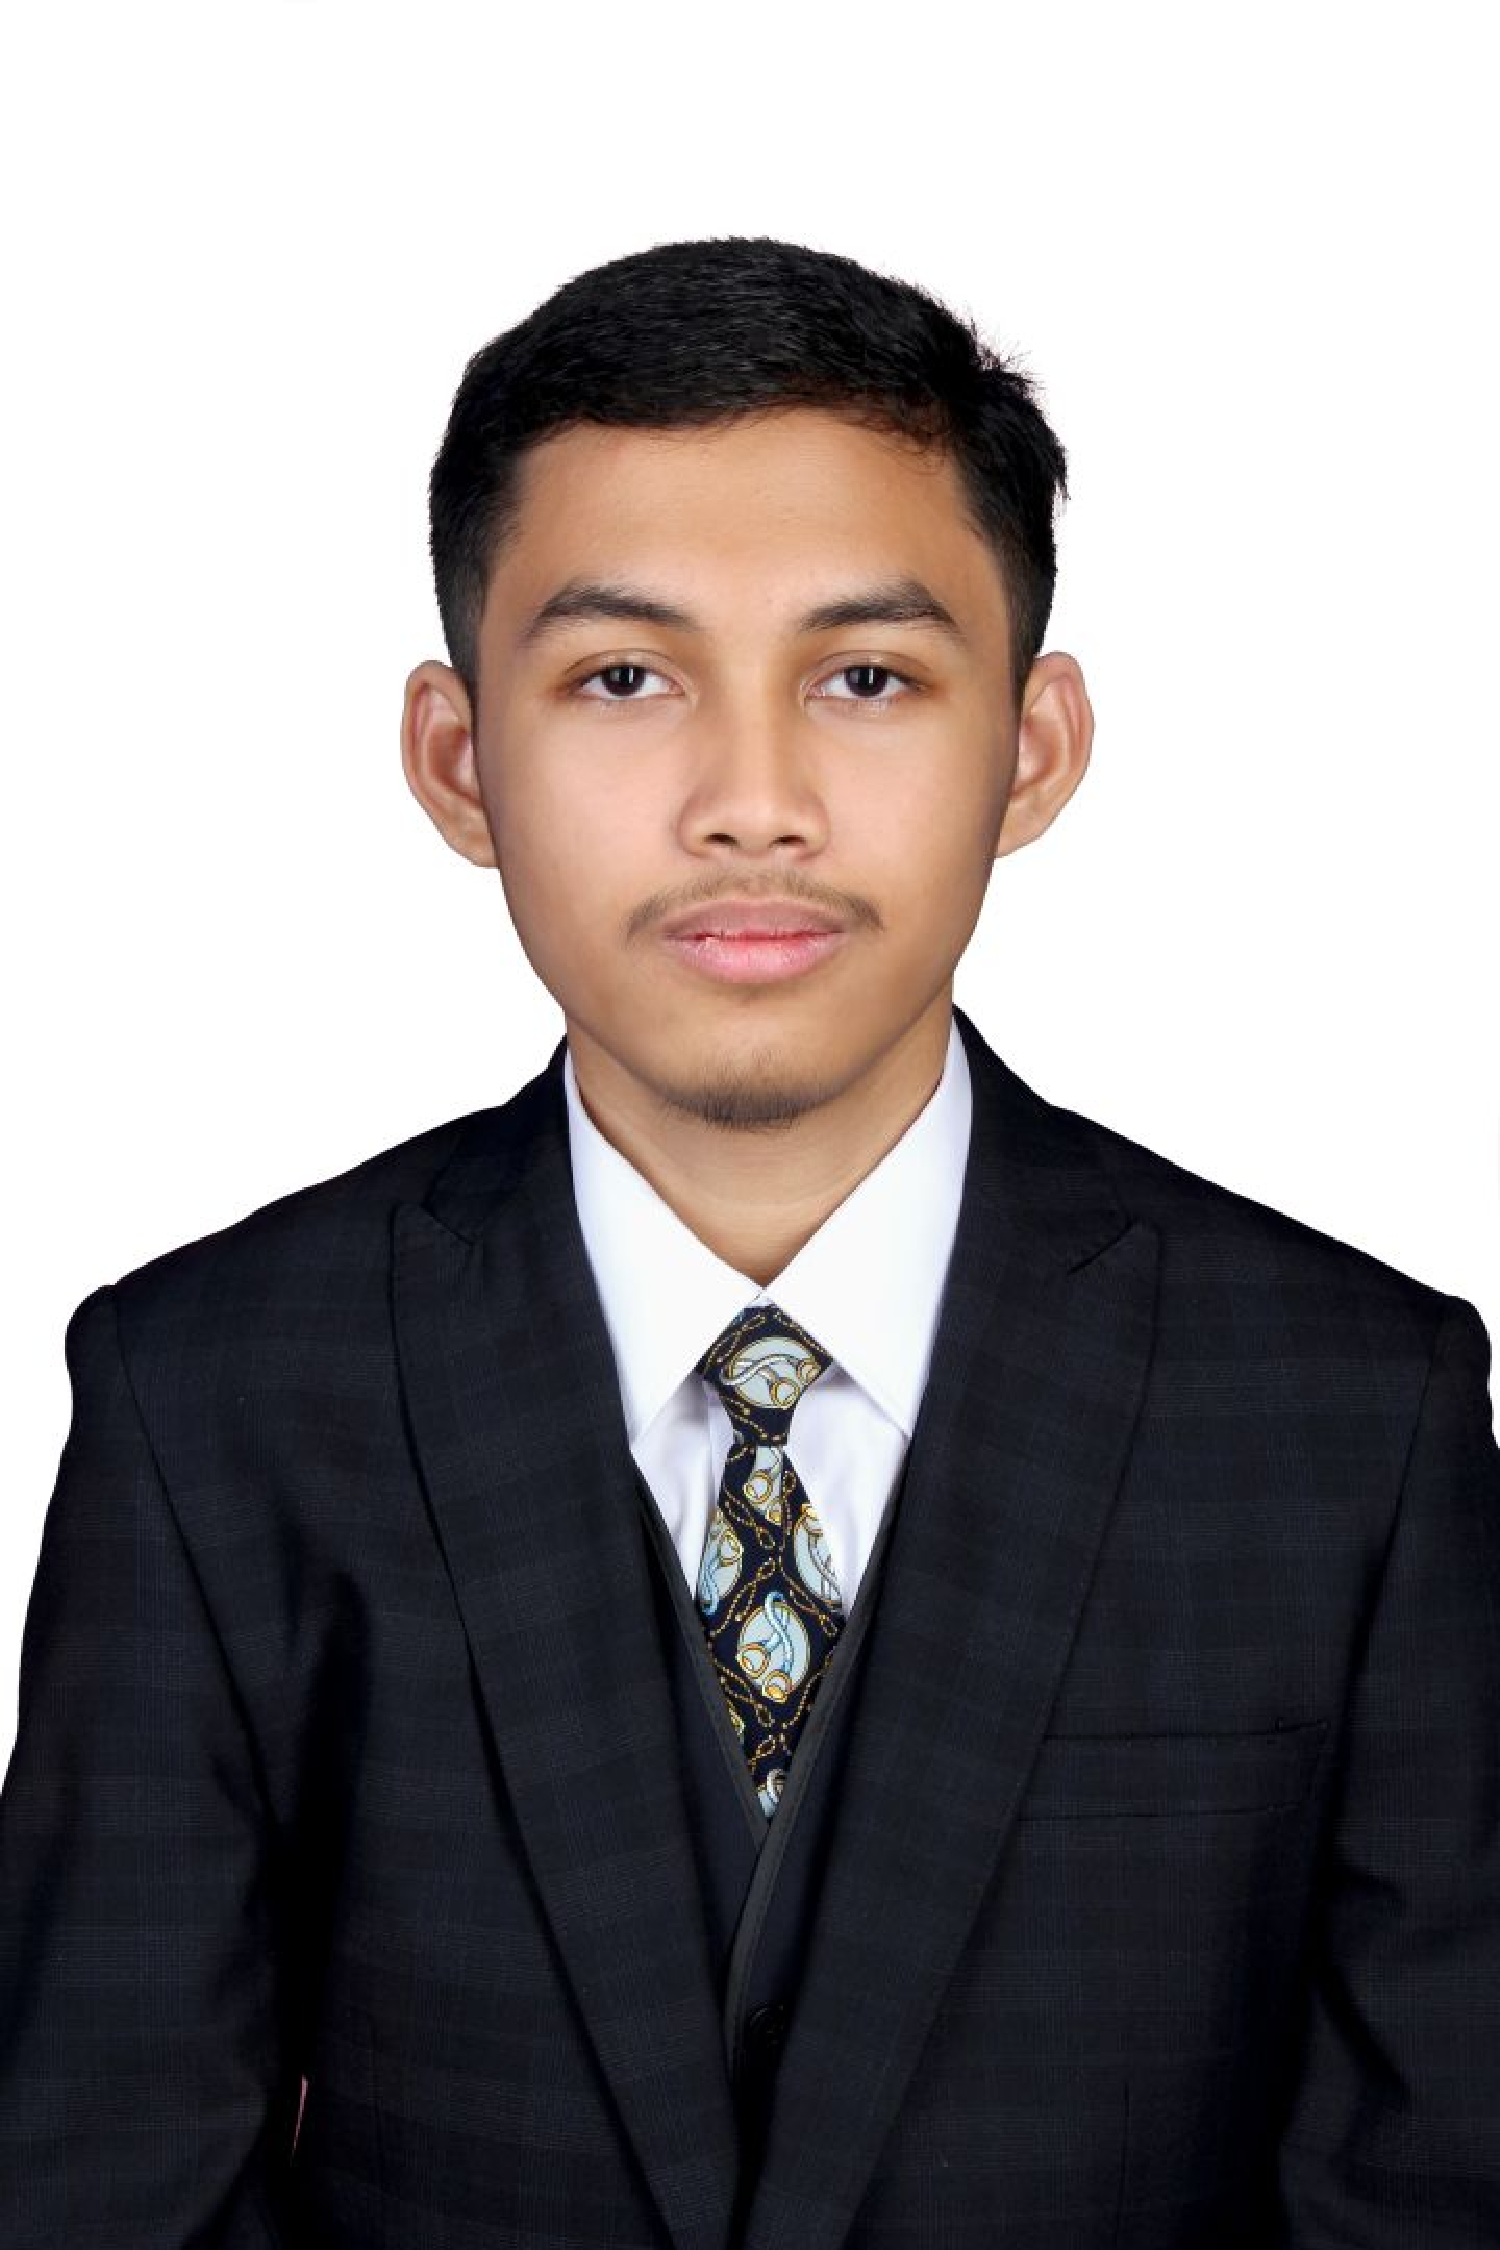
\includegraphics[width=\linewidth]{img/theAuthorPhoto}
	\vspace{-2em}
\end{wrapfigure}

Penulis dilahirkan di kota Surabaya pada tahun 2003, yang merupakan anak pertama dari 2 bersaudara. Penulis telah menempuh pendidikan formal melalui Paket A dari PKBM Siliwangi 2, Paket B dari PKBM Minda Utama, dan Paket C dari PKBM Pewaris Bangsa. Setelah lulus dari pendidikan menengah atas, penulis lanjut menempuh pendidikan sarjana di \departmentNameBahasa, \facultyNameBahasa, \campusName\ sejak tahun 2021, terdaftar dengan NRP \theAuthorId.

Di \departmentNameBahasa, penulis sempat aktif sebagai asisten praktikum mata kuliah Algoritma dan Pemrograman, serta Pemrograman Berorientasi Obyek. Selain itu, penulis juga pernah mengikuti pertukaran pelajar dari program Indonesian International Student Mobility Awards, sebagai mahasiswa dari \campusName\ yang menerima beasiswa, ke The University of Columbia, Canada, selama satu semester.

	\cleardoublepage
\end{document}
